% !TeX root = RJwrapper.tex
\title{Network Visualizations in \pkg{ggplot2}}
\author{by Sam Tyner, Fran\c{c}ois Briatte and  Heike Hofmann}

\maketitle
\abstract{
This paper explores three different approaches to visualize networks by building on the grammar of graphics framework implemented in the \pkg{ggplot2} package. The goal of each approach is to provide the user with the ability to apply the flexibility of \pkg{ggplot2} to the visualization of network data, including through the mapping of network attributes to specific plot aesthetics. We will show that these additions contribute significantly to the study of networks by making visualization of networks intuitive, both for users who are familiar with \pkg{ggplot2} and for those who are not.
}

% \hh{TODO list:
% 
% \begin{enumerate}
% 
% \item %%%%%%%%%%%%
%   \hh{start of end phase!!! Proof read. Check examples for consistency.}
% 
%   \fb{I have started moving some in-text comments to discussion or out when the problem that they flagged has been solved.}
% 
% \item %%%%%%%%%%%%
%   \hh{need to re-run the timing after all the changes are made to the packages. }
% 
%   \fb{I have included some testing code + prelim. results in the "runtimes" folder.}

% \item %%%%%%%%%%%%
%   \sct{check that the reference commands all make sense. for instance, section 2.1 is referenced at the top of page 3 but the sections aren't labeled with numbers in the paper. Is this something to do with the template for the R Journal? }
% \hh{good point - I've changed ref to nameref.}
%\end{enumerate}}






% introductory section
\par There are many kinds of networks, and networks are extensively studied across many disciplines \citep{watts2004ars}. For instance, social network analysis is a longstanding and prominent subfield of sociology, and the study of biological networks, such as protein-protein interaction networks or metabolic networks, is a notable subfield of biology \citep{prell2011social, junker2008analysis}. Though these two disciplines and the many others that study networks are themselves extremely different, they can all benefit from good network visualization methods.

% Visualization of networks helps with analysis
Coloring the vertices or edges in a graph is a quick way to visualize grouping and can help with pattern or cluster detection. The vertices in a network and the edges between them compose the structure of a network, and being able to visually discover patterns among them is a key part of network analysis. Viewing multiple layouts of the same network can also help reveal patterns or clusters that would not be discovered when only viewing one layout or analyzing only its underlying adjacency matrix.

% Many network packages exist, but are not easy to use
Many R packages already exist for network analysis and visualization such as \CRANpkg{igraph} by \citet{igraph}, \CRANpkg{sna} by \citet{sna}, and \CRANpkg{network} by \citet{network.jss, network}. Unfortunately, there is no standard format for network visualization across these packages. The user, therefore, must have detailed knowledge of each one of these packages in order to make meaningful changes to the network visualization. Customizing the colors, sizes, etc. of the vertices and edges of the network is done ``by hand'' and differently in each of these packages. For instance, the \pkg{igraph} package allows for coloring vertices by groups but the user has to assign the colors to each vertex individually as opposed to assigning color by a grouping factor variable.

% ggplot2 as an implementation framework
Our objective is to bring network plotting capabilities to the popular \CRANpkg{ggplot2} package \citep{ggplot2}. Wickham designed it as an implementation of the `grammar of graphics' proposed by \citet{wilkinson:1999}, and \pkg{ggplot2} has since become extremely popular among R users.%
\footnote{In order to give an indication of how  large the user base of \pkg{ggplot2} is, we looked at its usage statistics from January 1, 2015 to October 31, 2015 (see \url{http://cran-logs.rstudio.com/}). Over this period, the \pkg{ggplot2} package was downloaded over 1.3 million times from CRAN, which amounts to over 4,500 downloads per day. The package has been downloaded at least once in 216 countries, and in 22 of those countries, including China, Israel, and Colombia, it has been downloaded over 10,000 times.} %
%\sct{XXX I do not think that the line about Python is relevant, as we are submitting this to the R journal. I have commented it out for now. XXX}
  %to the point that it has even inspired a port of its syntax to the Python programming language, which is a rare achievement for an R package.%
  %
  %\footnote{See \url{http://ggplot.yhathq.com/}.} %
  % see also: port of ggplot2 to plotly? \url{https://plot.ly/ggplot2/} %% -- hh
  %
%  This is the audience we are aiming at by making network visualizations a part of \pkg{ggplot2}.
Because the syntax implemented in the \pkg{ggplot2} package is extendable to many different kinds of visualizations, many packages have built additional functionalities on top of the existing package. Examples include the \CRANpkg{ggmap} package by \citet{ggmap} for spatial visualization, the \CRANpkg{ggfortify} package by \citet{ggfortify} for visualizing statistical models, the package \CRANpkg{GGally} by \citet{ggally}, and the \BIOpkg{ggbio} Bioconductor package by \citet{ggbio}, which provides graphics for biological data.
These packages have expanded the utility of \pkg{ggplot2}, likely resulting in a great increase of its user base. We hope to add to this user base even more by extending the benefits of the grammar of graphics to network visualization.
% Just as these examples have increased the utility of \pkg{ggplot2}, our additions aim to extend the benefits of the grammar of graphics to network visualization.
Our efforts rely upon the most recent changes to \pkg{ggplot2}, which allow users to more easily extend the package through additional geometries or \samp{geoms}.%
\footnote{Version 1.1.0, released mid November 2015. See \url{https://cran.r-project.org/web/packages/ggplot2/NEWS} for the full list of changes in \pkg{ggplot2} 1.1.0, as well as the new package vignette, ``Extending ggplot2'', which explains how the internal \code{ggproto} system of object-oriented programming can be used to create new geoms.} %
  %

In the remainder of this paper, we present three different approaches to network visualization with \pkg{ggplot2}. Section~\nameref{sec:background} introduces the basic terminology of networks and illustrates their ubiquity in natural and social life. Section~\nameref{sec:implementations} then discusses the logic behind each of the three approaches that we offer. Section~\nameref{sec:examples} extends that discussion through several examples ranging from simple to complex networks, for which we provide the code corresponding to each approach alongside its graphical result. We follow with some considerations of runtimes in plotting networks in Section~\nameref{sec:speed} before closing with a discussion.

\section{A quick primer on network structures}
\label{sec:background}

In its essence, a network is simply a set of points connected in pairs by a set of lines \citep{newman}. Here, we refer to the lines as edges (or ties) and to the points as nodes (or vertices). We note that our examples are all one-mode networks, where all nodes are of the same kind and are able to connect to each other, however the graphical tools presented can be used to visualize more general types of networks. %\sct{XXX I'm not 100\% sure that's true but it seems right.XXX
% HH: more general is definitely true}

The two sets of graphical objects that make up a network, points and segments between them, have been used to encode a huge variety and quantity of information across many different fields of study. For instance, networks of scientific collaboration, a food web of marine animals, and American college football games are all covered in a paper on community detection in networks by \citet{football}. \citet{networkfailures} examine node failure in interdependent networks like power grids.  Social networks such as links between actors found on \url{http://www.imdb.com/} and neural networks, like the completely mapped neural network of the \textit{C. elegans} worm are also extensively studied \citep{smallworld}.

Networks can vary widely in scope and complexity: the smallest network is simply an edge between two vertices, while one of the most commonly used and most complex networks, the world wide web, has billions of vertices (Web pages) and billions of edges (hyperlinks) connecting them. Additionally, the edges in a network can be directed or undirected: directed edges represent information travelling from one vertex to another, and switching the direction would change the structure of the network. The World Wide Web is an example of a directed network because hyperlinks connect one Web page to another, but not necessarily the other way around. Undirected edges are simply connections between vertices. Co-authorship networks are examples of undirected networks, where nodes are authors and they are connected by an edge if they have written an academic publication together.

An even more common network example is a social network. A social network is a network that everyone is a part of in one way or another. We do not necessarily refer here to social media like Facebook or LinkedIn, but rather to the connections we form with other people. To demonstrate the functionality of our tools for plotting networks, we have chosen an example of a social network from the popular television show \emph{Mad Men}. This network, which was compiled by \citet{madmen}, is made up of 52 vertices and 87 edges. Each vertex represents a character on the show, and there is an edge between every two characters who have had a romantic relationship.

\begin{figure}[hbtp]
\centering

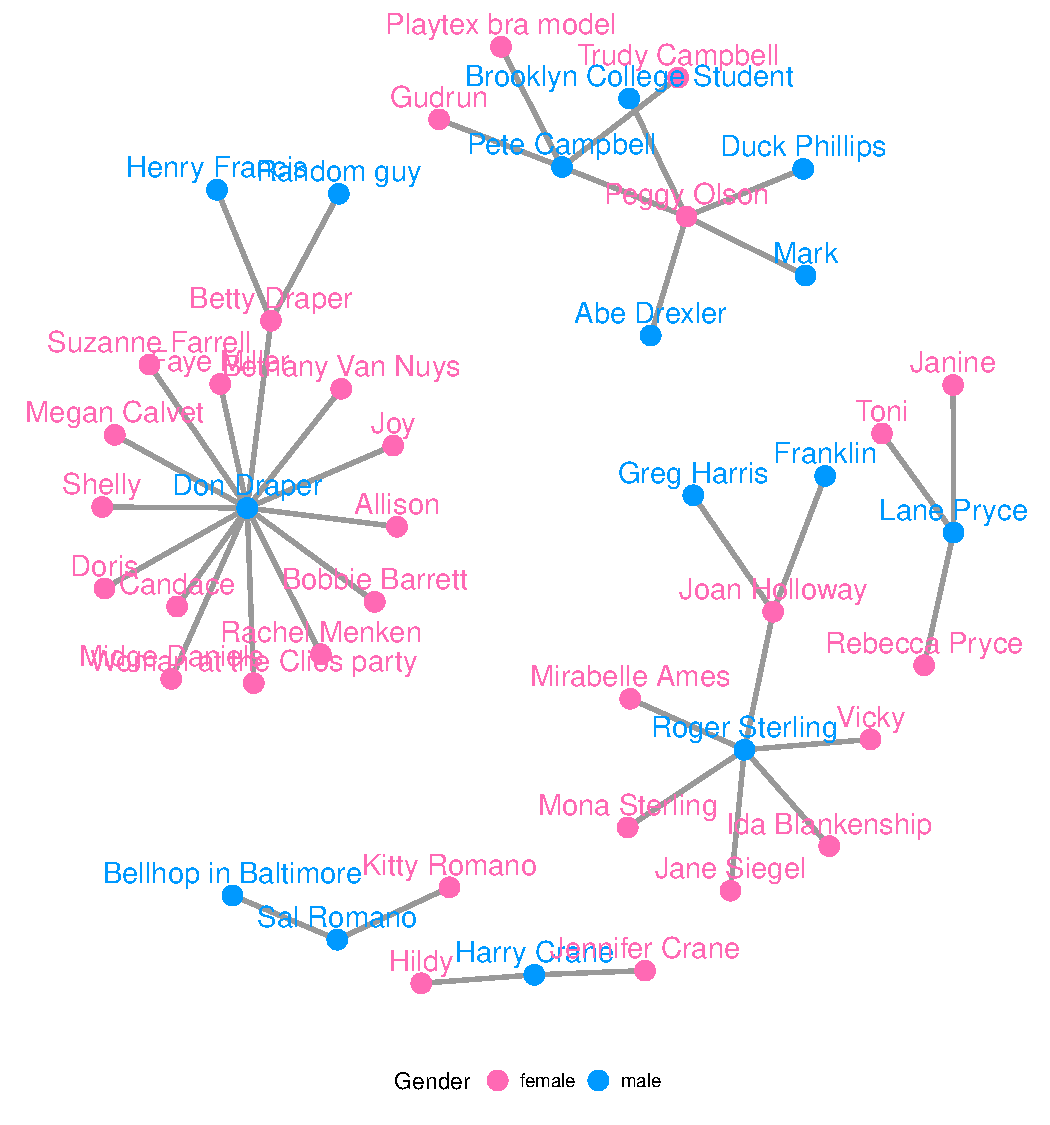
\includegraphics[width=0.6\textwidth]{figure/madmen_geom_net-1.pdf}
\caption{\label{fig.cap:madmen} Graph of the characters in the show Mad Men who are linked by a romantic relationship. }
\end{figure}
%%\afterpage{\clearpage}

Figure~\ref{fig.cap:madmen} shows this network. In the plot, we can see one central character who has many more relationships than any other character. This vertex represents the main character of the show, Don Draper, who is quite the ``ladies' man.'' Networks like this one, no matter how simple or complex, are everywhere, and we hope to provide the curious reader with a straightforward way to visualize any network they choose.
 % SCT I am not wild about this line:  %This example shows just how ubiquitous networks are.


% ==============================================================================
%
\section{Three implementations of network visualizations}%
\label{sec:implementations}
%
% ==============================================================================


We present two basic approaches to using the \pkg{ggplot2} framework for network visualization. First, we implement network visualizations by providing a wrapper function, \code{ggnet2} for the user to visualize a network using \pkg{ggplot2} elements. Second, we implement network visualizations using layering in \pkg{ggplot2}.  For the second approach, we have two ways of creating a network visualization. The first, \pkg{geomnet}, wraps all network structures, including vertices, edges, and vertex labels into a single \code{geom}. The second, \pkg{ggnetwork}, implements each structural component in an independent \code{geom} and layers them to create the visualization. We will discuss all of these approaches in this section.

\subsection{ggnet2} % ==========================================================

The \code{ggnet2} function is an improved version of the \code{ggnet} function, which has been part of the \pkg{GGally} package since 2013 \citep{ggally}. Both functions can be separately installed in the form of a small R package available from \url{https://github.com/briatte/ggnet}, and a detailed introduction to the \code{ggnet2} function is available from within the package as a vignette.%
\footnote{The vignette can be viewed online at \url{https://briatte.github.io/ggnet/}.}%

The \code{ggnet2} function offers a large range of network visualization functionalities in a single function call. Although its result is a \pkg{ggplot2} object that can be further styled with \pkg{ggplot2} scales and themes, the syntax of the \code{ggnet2} function is designed to be easily understood by the user. The aesthetics relating to the nodes are controlled by arguments such as \code{node.alpha} or \code{node.color}, while those relating to the edges are controlled by %similarly named
arguments starting with \samp{edge}. As a consequence, while \code{ggnet2} applies the grammar of graphics to network objects, the function itself still works very much like the plotting functions of the \pkg{igraph} and \pkg{network} packages: a long series of arguments is used to control every possible aspect of how the network should be visualized.

The \code{ggnet2} function takes a single network object as input. This initial object might be an object of class \code{"network"} (with the exception of hypergraphs or multiplex graphs), or any data structure coercible to an object of that class, such as an incidence matrix, an adjacency matrix, or an edge list. Additionally, if the \CRANpkg{intergraph} package \citep{intergraph} is installed, the function  also accepts a network object of class \code{"igraph"}. Internally, the function converts the network object to two data frames: one for edges and another one for nodes. It then passes them to \pkg{ggplot2}. Each of the two data frames contain the information required by \pkg{ggplot2} to plot segments and points respectively, such as a shape for the points (nodes) and a linetype for the segments (edges). The final result returned to the user is a plot with a minimum of two layers, or more if there are edge and/or node labels.%

The \code{mode} argument of \code{ggnet2} controls how the nodes of the network are to be positioned in the plot returned by the function. This argument can take any of the layout values supported by the \code{gplot.layout} function of the \pkg{sna} package, and defaults to \samp{fruchtermanreingold}, which places the nodes through the Fruchterman-Reingold layout algorithm \citep{fruchterman_reingold}. Many other possible layouts and their parameters can also be passed to \code{ggnet2} through the \code{layout.par} argument. For a list of possible layouts and their arguments, see \code{?sna::gplot.layout}.

Other arguments passed to the \code{ggnet2} function offer extensive control over the aesthetics of the plot that it returns, including %through
the addition of edge and/or node labels and their respective aesthetics.
Arguments such as \code{node.shape} or \code{edge.lty}, which  control the shape of the nodes and the linetype of the edges, respectively, can take a global value, such as \samp{15} %for \code{node.shape}
or \samp{dashed}% for \code{edge.lty},
a vector of global values, or the name of an edge or vertex attribute, in which case the values of that attribute are used as the mapping aesthetic.

This last functionality builds on one of the strengths of the \code{"network"} class, which can store %meta-
information on network edges and nodes as attributes that are then accessible to the user through the \code{\%e\%} and \code{\%v\%} operators respectively.%
%
\footnote{See \citet[p.~22-24]{network}. The equivalent operators in the \pkg{igraph} package are called \code{E} and \code{V}.} %
  %
  If the \code{ggnet2} function is given the \code{node.alpha = "importance"} argument, it will interpret it as an attempt to map the vertex attribute called \samp{importance} to the transparency level of the nodes. This works exactly like the command \code{net \%v\% "importance"}, which returns the vertex attribute \samp{importance} of the \code{"network"} object \code{net}. % SCT : This sentence seems very redundant. %This same result can also be achieved by passing the more explicit argument \code{node.alpha = net \%v\% "importance"}.
  This functionality allows the \code{ggnet2} function to work in a similar fashion to \pkg{ggplot2} mappings of aesthetics within the \code{aes} operator.

The \code{ggnet2} function also provides a few network-specific options, such as sizing the nodes as a function of their unweighted degree, or using the primary and secondary modes of a bipartite network as an aesthetic mapping for the nodes.%
\footnote{Bipartite (or 'two-mode') networks are networks with two different kinds of nodes and where all ties are formed between these two kinds. Affiliation networks, which represent the ties between individuals and the groups to which they belong, are examples of such networks \citep[see][p.~53-54 and p.~123-127]{newman}.}%
  %
All in all, the \code{ggnet2} function combines two different kinds of processes: it translates a network object into a data frame suitable for plotting with \pkg{ggplot2}, and it applies network-related aesthetic operations to that data frame, such as coloring the edges in function of the color of the nodes that they connect. %\sct{In the next section, we discuss \pkg{geomnet}, which is similarly constructed.}

\subsection{geomnet} % =========================================================

\subsubsection{Data Structure}

The package \pkg{geomnet} implements network visualization in a single \pkg{ggplot2} layer. It is available at \url{github.com/sctyner/geomnet}. The package has two main functions:  \code{stat\_net}, which performs all of the calculations, and \code{geom\_net}, which renders the plot.
The approach in \code{geomnet} is similar to the implementation of other, native \pkg{ggplot2} geoms, such as \code{geom\_smooth}. When using \code{geom\_smooth}, the user does not need to know about any of the internals of the loess function, and similarly, when using \code{geomnet}, the user is not expected to know about the internals of the layout algorithm, but only needs to specify the essential elements necessary for calculating a layout. On the other hand, if users are comfortable with network analysis, the entire body of layout methods provided by the \pkg{sna} package is available to them through the parameters \code{layout} and \code{layout.par}.
%
In network analysis there are usually two sources of information: one data set consisting of a description of the actors, represented as the vertices in the network, and another data set detailing the relationship between these actors, the edge dataset. We make two important assumptions about the way this information is encoded. First, we assume that the vertices are labelled using an `id' column. Second, we assume that the edges are described as connection between vertices via their respective `id' labels in a `from' and a `to' column. Thus, the minimum amount of information needed is a vector of all vertex labels and a two column data frame of to and from vertex ids corresponding to the edges.  In order for this geometry to work, these two data sets need to be combined into a single data frame. For this, we are using the convention that all of the vertex information is merged into the edge data set using the `from' as the reference column in a full join operations. Generally, there will be some vertices that are sinks in the network because they only show up in the `to' column. We can easily accommodate for these by adding artificial edges in the data set that have missing information for the `to' column.

Fortunately, R provides functionality that allows for an easy way of producing the required result: \code{merge} (in base R), \code{join} \citep[in \CRANpkg{plyr} see][]{plyr} and \code{full\_join} \citep[in \CRANpkg{dplyr}, see][]{dplyr} can be used. In \code{merge} the argument \code{all} needs to be set to \code{TRUE}; in \code{join}, the parameters have to be set to \code{type = "full"} and \code{all = TRUE}. These operations are equivalent to a `full join' in SQL terminology.

The formal requirements of \code{stat\_net} are two columns, called \code{from\_id} and \code{to\_id}. During this routine, columns \code{x, y} and \code{xend, yend} are calculated and used as a required input for \code{geom\_net}.
%
Other variables may also be included for each edge, such as the edge weight, in-degree, out-degree or grouping variable.

\subsubsection{Parameters and aesthetics}

Parameters that are currently implemented in \code{geom\_net} are:

\begin{itemize}
\item {\bf layout:}
the \code{layout} parameter takes a character value corresponding to the possible layouts in the \pkg{sna} package that are available within the \code{gplot.layout.*()} family of functions.  The default layout is the Kamada-Kawai layout, a force-directed layout for undirected networks \citep{kamadakawai}.
% removed a sentence here to include it above in description of ggnet2
% sorry for blatant act of sentence piracy!
Corresponding to each layout, the parameter  \code{layout.par} consists of a list of the parameters for the chosen layout. \code{fiteach} is a logical value specifying whether each panel's data should be fit separately (default) or whether the same layout should be used for all of the panels.
\item {\bf vertices:} any of \pkg{ggplot2}'s aesthetics relating to points: colour, size, shape, and alpha are available and used for specifying the appearance of nodes in the network.
%
\item {\bf edges:} for edges we distinguish between two different sets of aesthetics: aesthetics that only relate to line attributes, such as  linewidth, linetype, and stroke.  These can be used in the regular way.  Additionally, node aesthetics such as alpha or colour are used for vertices unless separately spcified by using the parameters \code{ecolour} or \code{ealpha}, which are only applied to the edges. If the \code{group} variable is specified, a new variable, called \code{samegroup} is added during the layout process. This variable is \code{TRUE}, if an edge is between two vertices of the same group, and \code{FALSE} otherwise. If \code{samegroup} is \code{TRUE}, the corresponding edge will be colored using the same color as the vertices it connects. If the edge is between vertices of a different group, a default grey shade is used for the edge.

The parameter \code{curvature} is set to zero by default, but if specified, leads to curved edges using the newly implemented \pkg{ggplot2} geom \code{geom\_curve} instead of the regular \code{geom\_segment}.
Note that the edge specific aesthetics that overwrite node aesthetics are currently considered as `as.is' values: they do not get a legend and are not scaled within the ggplot2 framework. This is done to avoid any clashes between node and edge scales.

{\bf self-referencing vertices:} some networks contain self references, i.e.\  an edge has the same vertex id in its from and to columns. If the parameter \code{selfies} is set to \code{TRUE}, a circle is drawn next to the vertex to represent this self reference.

%
\item {\bf arrow:} whenever the parameter \code{directed} is set from its default state to \code{TRUE}, arrows are drawn from the `from' to the `to' node, with tips pointing towards the `to' node.  By default, arrows have an absolute size of 10 points. The parameter \code{arrowsize} consists of a positive numeric value that is used as a multiple of the original arrow size, i.e.\ \code{arrowsize = 2} shows arrow tips at twice their original size. In order to avoid overplotting of the arrow tips by the nodes, the parameter \code{arrowgap} can be used. \code{arrowgap} specifies a proportion by which the edge should be shrunk with default of 0.05. A value of 0.5 will result in edges drawn only half way from the `from' node to the `to' node.
\item {\bf labels:}  \code{label} can be used as either a logical parameter or as a data variable, in which case it is assumed that the associated variable consists of the character strings to be used for labeling the nodes. Again, if \code{colour} is specified for the nodes, the same values are used for the labels, unless \code{ labelcolour} is specified. Other parameter values, such as \code{vjust} and \code{hjust} help in adjusting labels relative to the nodes. The parameters work in the same fashion as in native \pkg{ggplot2} geoms.

\end{itemize}

\subsection{ggnetwork} % =======================================================

\pkg{ggnetwork} is a small R package that mimicks the behaviour of \code{geomnet} by defining several geoms to achieve similar results. The package can be installed from \url{https://github.com/briatte/ggnetwork} and is fully documented in the package vignette.%
%
\footnote{The vignette can be viewed online at \url{https://briatte.github.io/ggnetwork/}.}%

The approach taken by the \pkg{ggnetwork} package is to alias some of the native geoms of the \pkg{ggplot2} package, an aliased geom is simply a variant of an already existing one. The \pkg{ggplot2} package contains several examples of aliased geoms, such as \code{geom\_histogram}, which is a variant of \code{geom\_bar} see \citep[see][p.~67, Table~4.6]{ggplot2}.

Following that logic, the \pkg{ggnetwork} package adds four aliased geometries to \pkg{ggplot2}:

\begin{itemize}
  \item \code{geom\_nodes}, an alias to \code{geom\_point};
  \item \code{geom\_edges}, an alias to either \code{geom\_segment} or \code{geom\_curve};
  \item \code{geom\_nodetext}, an alias to \code{geom\_text}; and
  \item \code{geom\_edgetext}, an alias to \code{geom\_label}.
\end{itemize}

The four geoms are used to plot nodes, edges, node labels and edge labels, respectively. Two of the geoms that they alias, \code{geom\_curve} and \code{geom\_label}, are part of the new geometries introduced in \pkg{ggplot2} version 1.1.0. All four geoms behave exactly like those that they alias, and take exactly the same arguments. The only exception to that rule is the special case of \code{geom\_edges}, which accepts both the arguments of \code{geom\_segment} and those of \code{geom\_curve}; if its \code{curvature} argument is set to anything but \code{0} (the default), then \code{geom\_edges} behaves exactly like \code{geom\_curve}; otherwise, it behaves exactly like \code{geom\_segment}.

Just like the \code{ggnet2} function, the \pkg{ggnetwork} package takes a single network object as input. This can be an object of class \code{"network"}, some data structure coercible to that class, or an object of class \code{"igraph"} when the \pkg{intergraph} package is installed. This object is passed to the `workhorse' function of the package, which is also called \code{ggnetwork} to create a data frame, and then to the \code{data} argument of \code{ggplot()}.

Internally, the \code{ggnetwork} function starts by computing the \code{x} and \code{y} coordinates of all nodes in the network with respect to its \code{layout} argument, which defaults to the Fruchterman-Reingold layout algorithm \citep{fruchterman_reingold}. It then extracts the edge list of the network, to which it adds the coordinates of the sender and receiver nodes as well as all edge-level attributes. The result is a data frame with as many rows as there are edges in the network, and where the \code{x}, \code{y}, \code{xend} and \code{yend} hold the coordinates of the network edges.

At that stage, the \code{ggnetwork} function, like the \code{geomnet} package, performs a left-join of that augmented edge list with the vertex-level attributes of the %sender
`from' nodes. It also adds one self-loop per node, in order to ensure that every node is plotted even when their degree is zero---that is, even if the node is not connected to any other node of the network, and is therefore absent from the edge list. The data frame created by this process contains one row per edge as well as one additional row per node, and features all edge-level and vertex-level attributes initially present in the network.%
% SCT: I don't think we should have this footnote because it doesn't quite seem necessary.
\footnote{One limitation of this process is that it requires some reserved variable names (\code{x}, \code{y}, \code{xend} and \code{yend}), which should not also be present as edge-level or vertex-level attributes (otherwise the function will simply break). Similarly, if an edge attribute and a vertex attribute have the same name, like  \samp{na}, which the \pkg{network} package defines as an attribute for both edges and vertices in order to flag missing data, \code{ggnetwork} will rename them to \samp{na.x} (for the edge-level attribute) and \samp{na.y} (for the vertex-level attribute).} %

The \code{ggnetwork} function also accepts the arguments \code{arrow.gap} and \code{by}. Like in \pkg{geomnet}, \code{arrow.gap} slightly shortens the edges of directed networks in order to avoid overplotting edge arrows and nodes. The argument \code{by} is intended for use with plot facets. Passing an edge attribute as a grouping variable to the \code{by} argument will cause \code{ggnetwork} to return a data frame in which each node appears as many times as there are unique values of that edge attribute, using the same coordinates for all occurrences. When that same edge attribute is also passed to either \code{facet\_wrap} or \code{facet\_grid}, each edge of the network will show in only one panel of the plot, and all nodes will appear in each of the panels at the same position. This makes the panels of the plot comparable to each other, and allows the user to visualize %edge formation
the network structure as a function of a specific edge attribute, like a temporal attribute.

Both the \code{arrow.gap} and the \code{by} arguments are further illustrated in the remainder of this paper.


% ==============================================================================
%
\section{Examples}%
\label{sec:examples}
%
% ==============================================================================


In this section, we demonstrate the current capabilities of \code{ggnet2}, \code{geomnet}, and \code{ggnetwork} in a series of side by side examples. While the output is similar for each method of network visualization, the code and implementations differ across the three methods.
For each of these examples, we are going to present the code necessary to produce the network, and discuss each application in detail.

\subsection{Blood donation}  % =================================================

In this directed network, there are eight vertices and 27 edges.  The vertices represent the eight different blood types in humans that are most important for donation: the ABO blood types A, B, AB, and O, combined with the RhD positive (+) and negative (-) types. The edges are directed: a person whose blood type is that of a \emph{from} vertex can to donate blood to a person whose blood type is that of a corresponding \emph{to} vertex.  This network is shown in Figure~\ref{fig.cap:blood}. The code to produce each one of the networks is shown below:

% \begin{figure}[hbtp]
% \caption{\label{tab:blood}Code for the three different approaches showing the blood donation network of figure~\ref{fig.cap:blood}.}


%
\begin{knitrout}
\definecolor{shadecolor}{rgb}{1, 1, 1}\color{fgcolor}\begin{kframe}
\begin{verbatim}
# plot with ggnet2
ggnet2(network(blood$edges[, 1:2]), mode = "circle", size = 15,
       label = TRUE, arrow.size = 10, arrow.gap = 0.05, vjust = 0.5,
       node.color = "darkred", label.color = "grey80")
\end{verbatim}
\end{kframe}
\end{knitrout}

\begin{knitrout}
\definecolor{shadecolor}{rgb}{1, 1, 1}\color{fgcolor}\begin{kframe}
\begin{verbatim}
# plot with geomnet
ggplot(data = blood$edges, aes(from_id = from, to_id = to)) +
  geom_net(colour = "darkred", layout = "circle", label = TRUE, size = 15,
           directed = TRUE, vjust = 0.5, labelcolour = "grey80",
           arrowsize = 1.5, linewidth = 0.5, arrowgap = 0.05,
           selfies = TRUE, ecolour = "grey40") +
  theme_net()
\end{verbatim}
\end{kframe}
\end{knitrout}

\begin{knitrout}
\definecolor{shadecolor}{rgb}{1, 1, 1}\color{fgcolor}\begin{kframe}
\begin{verbatim}
# plot with ggnetwork
ggplot(ggnetwork(network(blood$edges[, 1:2]),
                 layout = "circle", arrow.gap = 0.05),
       aes(x, y, xend = xend, yend = yend)) +
  geom_edges(color = "grey50",
             arrow = arrow(length = unit(10, "pt"), type = "closed")) +
  geom_nodes(size = 15, color = "darkred") +
  geom_nodetext(aes(label = vertex.names), color = "grey80") +
  theme_blank()
\end{verbatim}
\end{kframe}
\end{knitrout}

In this example every vertex has a self-reference, as blood between two people of matching ABO and RhD type can always be exchanged.  The \pkg{geomnet} approach shows these self-references as circles looping back to the vertex, which is controlled by using the parameter setting \code{selfies = TRUE}.

\begin{figure}[hbt]
\begin{subfigure}[t]{.32\textwidth}
\caption{ggnet2}
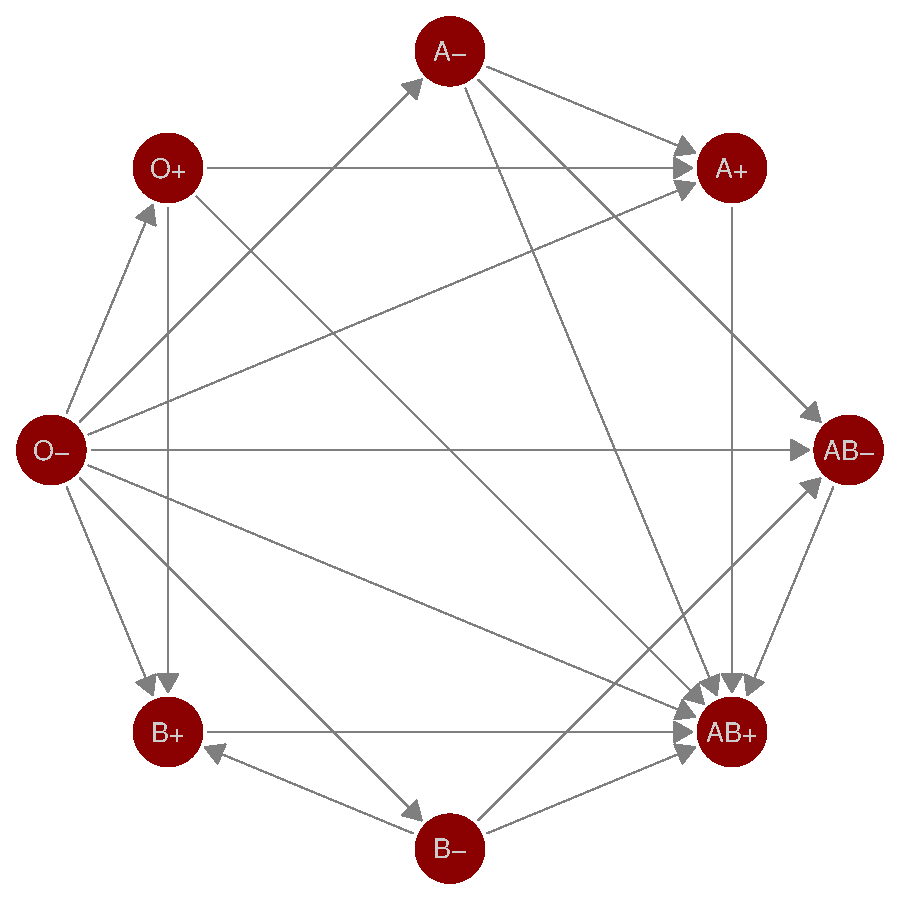
\includegraphics[width=\textwidth]{figure/blood_ggnet2-1.pdf}
\end{subfigure}
\begin{subfigure}[t]{.32\textwidth}
\caption{geomnet}
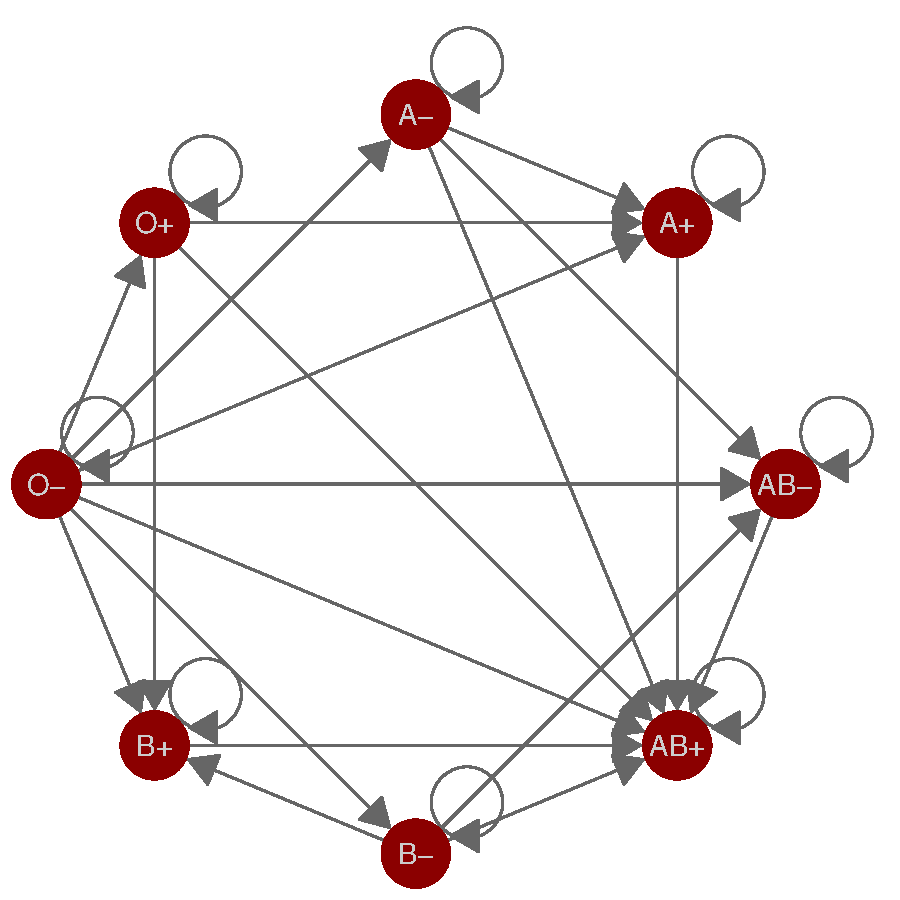
\includegraphics[width=\textwidth]{figure/blood_geom_net-1.pdf}
\end{subfigure}
\begin{subfigure}[t]{.32\textwidth}
\caption{ggnetwork}
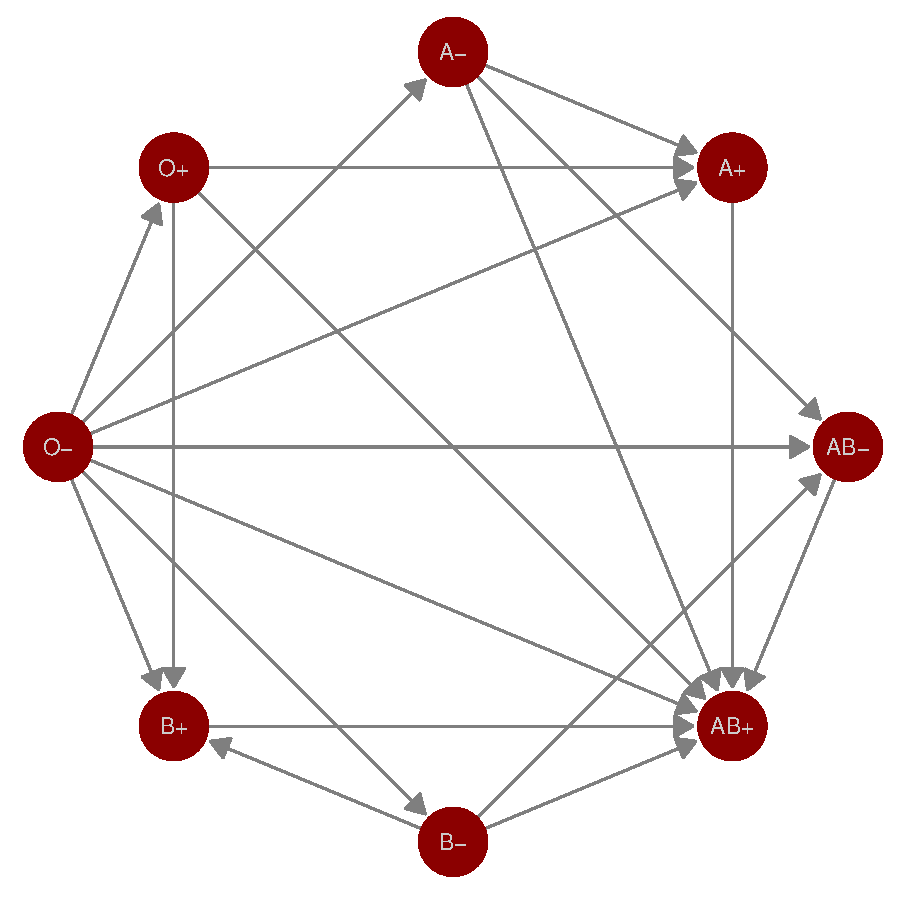
\includegraphics[width=\textwidth]{figure/blood_ggnetwork-1.pdf}
\end{subfigure}
\caption{\label{fig.cap:blood} Network of blood donation possibilities in humans by ABO and RhD blood types.}
\end{figure}
%%\afterpage{\clearpage}

\code{colour} and \code{size} aesthetics in Figure~\ref{fig.cap:blood} are set to identity values to change the size and color of all vertices. We have also used the \code{layout} and \code{label} arguments to change the default layout to a circle layout and to print the blood types, respectively. The circle layout places blood types of the same ABO type next to each other and spreads the vertices out far enough to distinguish between the various ``in" and ``out" types.  We can tell clearly from this plot that the O- type is the universal donor: it has an out-degree of seven and an in-degree of zero. Additionally, we can see that the AB+ type is the universal recipient, with an in-degree of seven and an out-degree of zero. Anyone looking at this plot can quickly determine which type(s) of blood they can receive and which type(s) can receive their blood.

\subsection{Email network} % ===================================================

\begin{figure}[hbt]
\begin{subfigure}[t]{\textwidth}
\caption{ggnet2}
\vspace{1em}

             \begin{adjustbox}{valign=t}

             \begin{minipage}{.49\textwidth}
 \begin{knitrout}\footnotesize
\definecolor{shadecolor}{rgb}{1, 1, 1}\color{fgcolor}\begin{kframe}
\begin{verbatim}
em.cet <- as.character(
  email$nodes$CurrentEmploymentType)
names(em.cet) = email$nodes$label

edges <- subset(email$edges, nrecipients < 54)
em.net <- edges[, c("From", "to") ]
em.net <- network(em.net)
em.net %v% "curr_empl_type" <-
  em.cet[ network.vertex.names(em.net) ]

ggnet2(em.net, color = "curr_empl_type",
       size = 4, palette = "Set1",
       arrow.size = 5, arrow.gap = 0.02,
       edge.alpha = 0.25,
       edge.color = c("color", "grey50"),
       color.legend = "Employment Type") +
  theme(legend.position = "bottom")
\end{verbatim}
\end{kframe}
\end{knitrout} \vspace{1em}

                   \end{minipage}

                  \begin{minipage}{.49\textwidth}

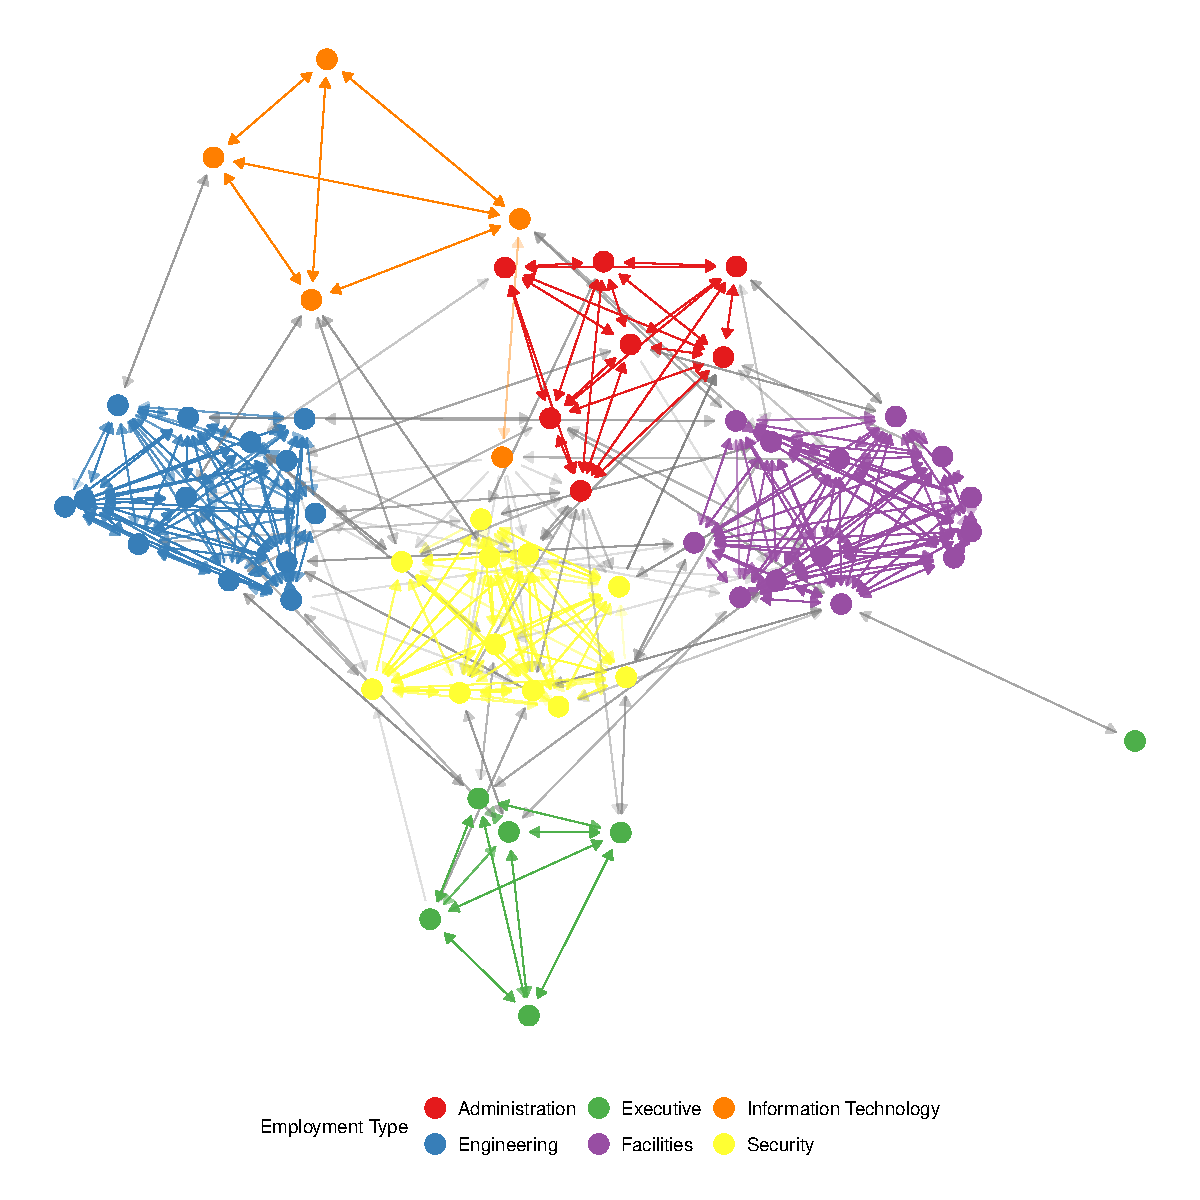
\includegraphics[width=\textwidth]{figure/email_ggnet2-1.pdf}

                          \end{minipage}

                          \end{adjustbox}

\end{subfigure}
%
\begin{subfigure}[t]{\textwidth}
\caption{geomnet}
\vspace{1em}

             \begin{adjustbox}{valign=t}

             \begin{minipage}{.49\textwidth}
 \begin{knitrout}\footnotesize
\definecolor{shadecolor}{rgb}{1, 1, 1}\color{fgcolor}\begin{kframe}
\begin{verbatim}
emailnet <- merge(
  subset(email$edges, nrecipients < 54),
  email$nodes,
  by.x = "From", by.y = "label", all = TRUE)

ggplot(data = emailnet,
       aes(from_id = From, to_id = to)) +
  geom_net(
    aes(colour = CurrentEmploymentType,
        group = CurrentEmploymentType,
        linewidth = 3 * (...samegroup.. / 8 + .125)),
    ealpha = 0.25,
    size = 4, curvature = 0.05,
    directed = TRUE, arrowsize = 0.5) +
  scale_colour_brewer("Employment Type", palette = "Set1") +
  theme_net() +
  theme(legend.position = "bottom")
\end{verbatim}
\end{kframe}
\end{knitrout} \vspace{1em}

                   \end{minipage}

                  \begin{minipage}{.49\textwidth}

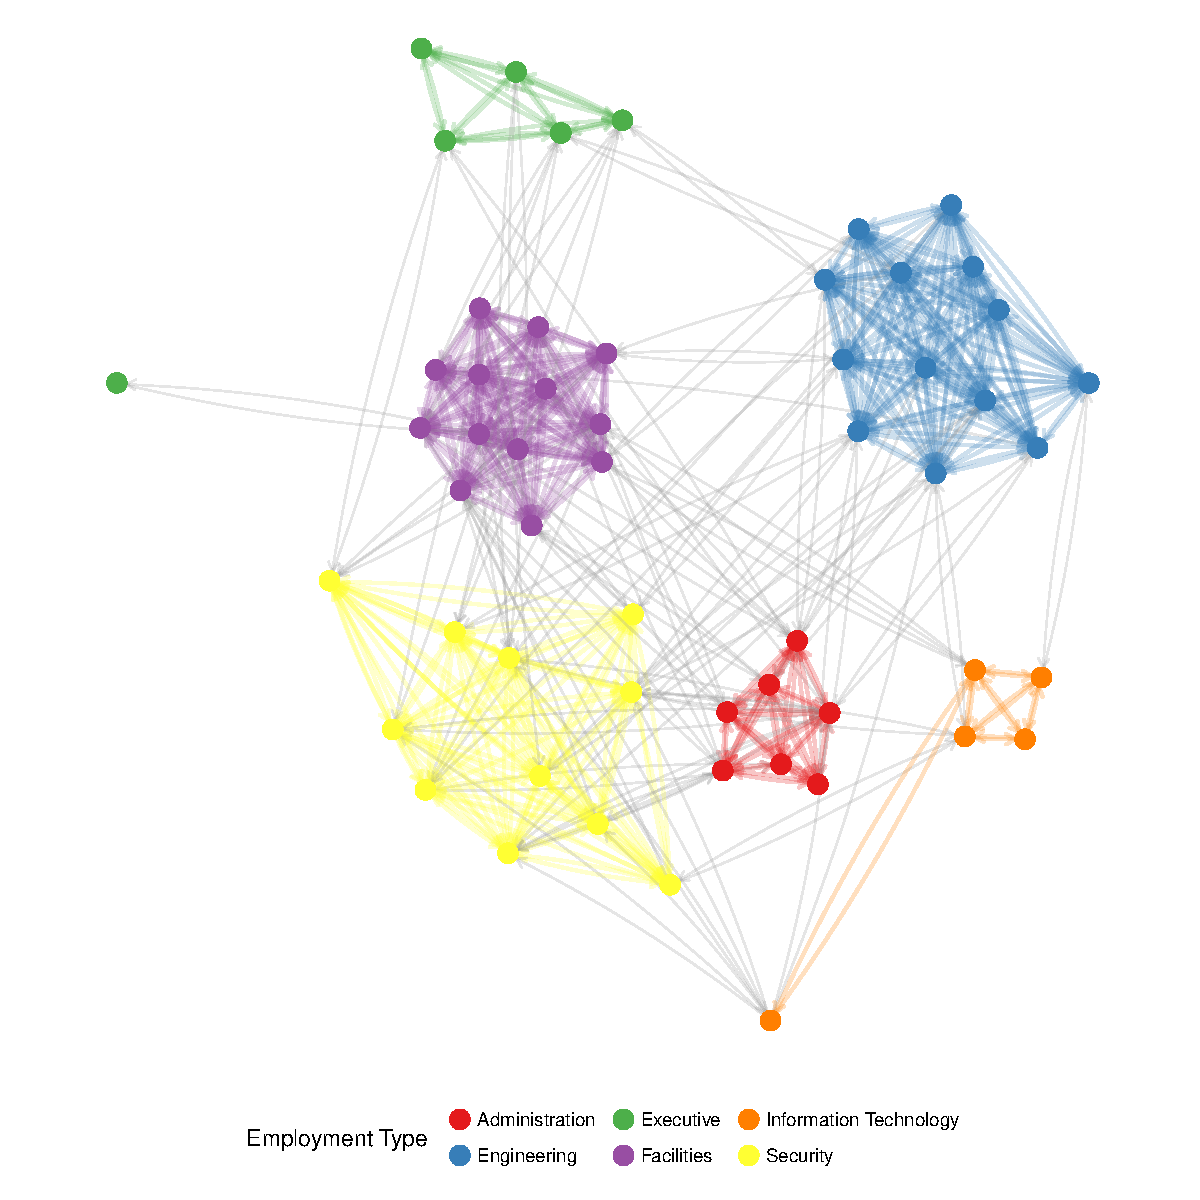
\includegraphics[width=\textwidth]{figure/email_geom_net-1.pdf}

                          \end{minipage}

                          \end{adjustbox}
\end{subfigure}
%
\begin{subfigure}[t]{\textwidth}
\caption{ggnetwork}
\vspace{1em}

             \begin{adjustbox}{valign=t}

             \begin{minipage}{.49\textwidth}
 \begin{knitrout}\footnotesize
\definecolor{shadecolor}{rgb}{1, 1, 1}\color{fgcolor}\begin{kframe}
\begin{verbatim}
ggplot(ggnetwork(em.net, arrow.gap = 0.02),
       aes(x, y, xend = xend, yend = yend)) +
  geom_edges(
    aes(color = curr_empl_type),
    alpha = 0.25,
    arrow = arrow(length = unit(5, "pt"),
                  type = "closed"),
    curvature = 0.05) +
  geom_nodes(aes(color = curr_empl_type),
             size = 4) +
  scale_color_brewer("Employment Type",
                     palette = "Set1") +
  theme_blank() +
  theme(legend.position = "bottom")
\end{verbatim}
\end{kframe}
\end{knitrout} \vspace{1em}

                   \end{minipage}

                  \begin{minipage}{.49\textwidth}

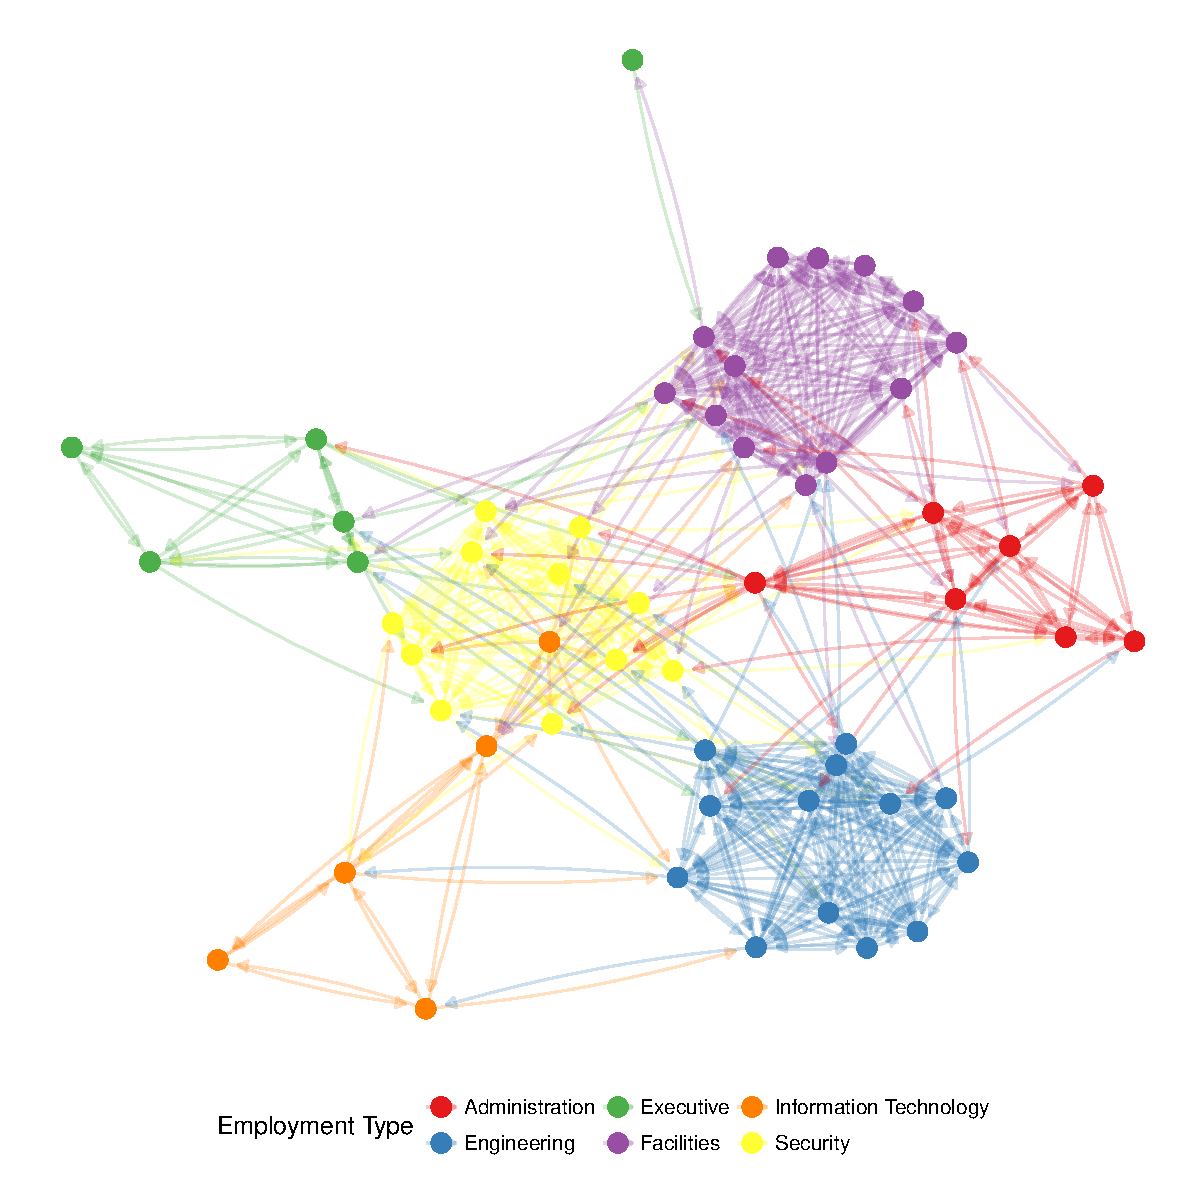
\includegraphics[width=\textwidth]{figure/email_ggnetwork-1.pdf}

                          \end{minipage}

                          \end{adjustbox}
\end{subfigure}

\caption{\label{fig.cap:email} Email network within a company over a two week period.}
\end{figure}
\afterpage{\clearpage}

The email network comes from the 2014 VAST Challenge \citep{emailnet}. It is a directed network of emails between company employees with 55 vertices and 9,063 edges. Each vertex represents an employee of the company, and each edge represents an email sent from one employee to another. The arrow of the directed edge points to the recipient(s) of the email. The network contains two business weeks of emails across the entire company. In order to better visualize the structure of the communication network between employees, emails that were sent out to all employees are removed.

% let's have all of the interpretation in a single place to simplify the flow
This network is plotted in Figure~\ref{fig.cap:email}. There are six distinct clusters in this network which almost perfectly correspond to the six different types of employees in this company: administration, engineering, executive, facilities, information technology, and security.

%% HH: this is not necessarily true anymore, when taking the number of emails exchanged into account. SCT: I agree.
%It is interesting to observe that, in all of the layouts, the `Security' employee group plays a central role in the email network of the company. This observation holds regardless of the actual network layout used (remember that \code{ggnet2} and \code{ggnetwork} default to the Fruchterman-Reingold algorithm, while \code{geomnet} defaults to the Kamada-Kawai algorithm; both layouts are force-directed, but proceed differently to assign coordinates to the nodes).
We can clearly see the varying densities of communications within departments and the more sparse communication between employees in different departments. We also see that one of the executives only communicates with employees in Facilities, while one of the IT employees frequently communicates with security employees.

A comparison of the results of \pkg{ggnet}, \pkg{geomnet} and \pkg{ggnetwork} reveals some of the %(subtle)
differences that exist between the implementations:

\begin{itemize}

  %% this paragraph has been fixed to reflect your (sct + hh) remarks -- fb

  \item %
  In the \code{ggnet2} implementation, the opacity of the edges between employees in the same cluster is higher than it is for the edges between employees in different clusters. This is due to the fact that the email network does not feature edge weights: instead, every email between two employees is represented by a different edge, resulting in edge overplotting. As the \code{edge.alpha} argument has been set to a value smaller than one, multiple emails between two employees create more opaque edges between them. This effect is not visible in the layouts created by \pkg{geomnet} and \code{ggnetwork} because both implementations draw a single segment for each directed edge, regardless of how many of these edges exist in the network data.

  \item %
  In the first two layouts of Figure~\ref{fig.cap:email}, edges between employees who share the same employment type are given the color of that employment type, while edges between employees belonging to different types are plotted in grey. This feature is particularly useful to visualize the amount of within-group connectedness in a network. By contrast, in the last layout, edges are colored according to the sender's employment type, because the \code{ggnetwork} package does not support coloring edges as a function of node-level attributes.

	\item %
	  Finally, in the last two layouts of Figure~\ref{fig.cap:email}, the \code{curvature} argument has been set to 0.05, resulting in slightly curved edges in both plots. This feature, which takes advantage of the \code{geom\_curve} geometry released in \pkg{ggplot2} 1.1.0, makes it possible to visualize which edges correspond to reciprocal connections; in an email communication network, as one might expect, most edges fall into that category.

\end{itemize}

To visualize how this network  changes over time, we facet the network by day: each panel in Figure~\ref{fig:email_facet} shows email networks associated with each day of the work week. The code for these visualization is below.

\begin{figure}[hbt]
\begin{subfigure}[t]{\textwidth}
\caption{ggnet2}\label{email:ggnet2}
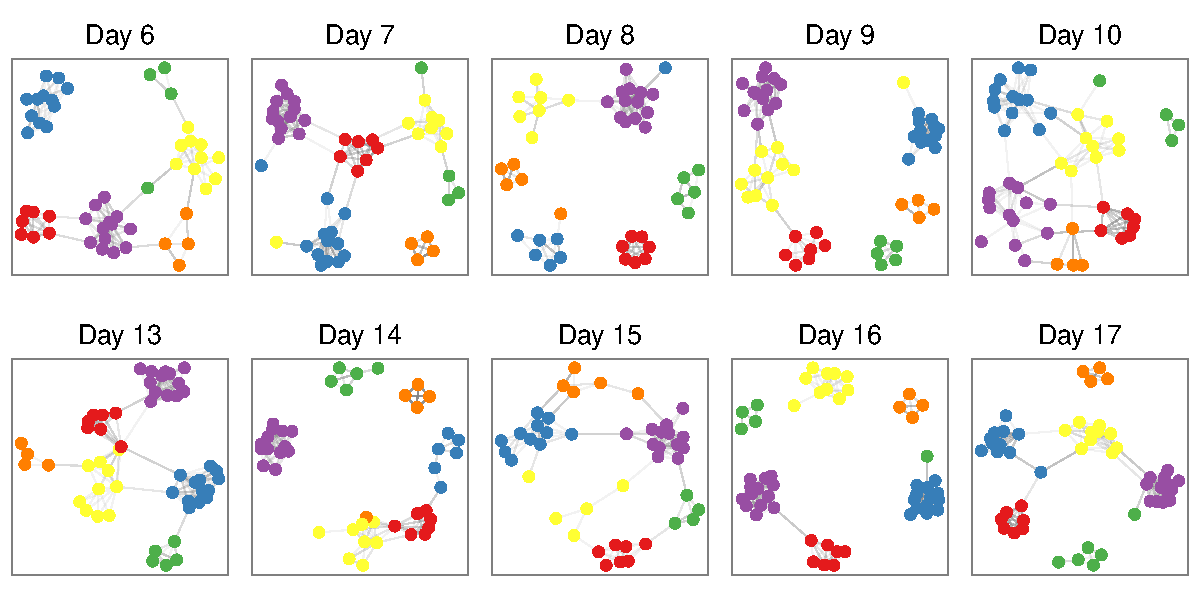
\includegraphics[width=\textwidth]{figure/email_facet_ggnet2-1.pdf}
\end{subfigure}
%
\begin{subfigure}[t]{\textwidth}
\caption{geomnet}
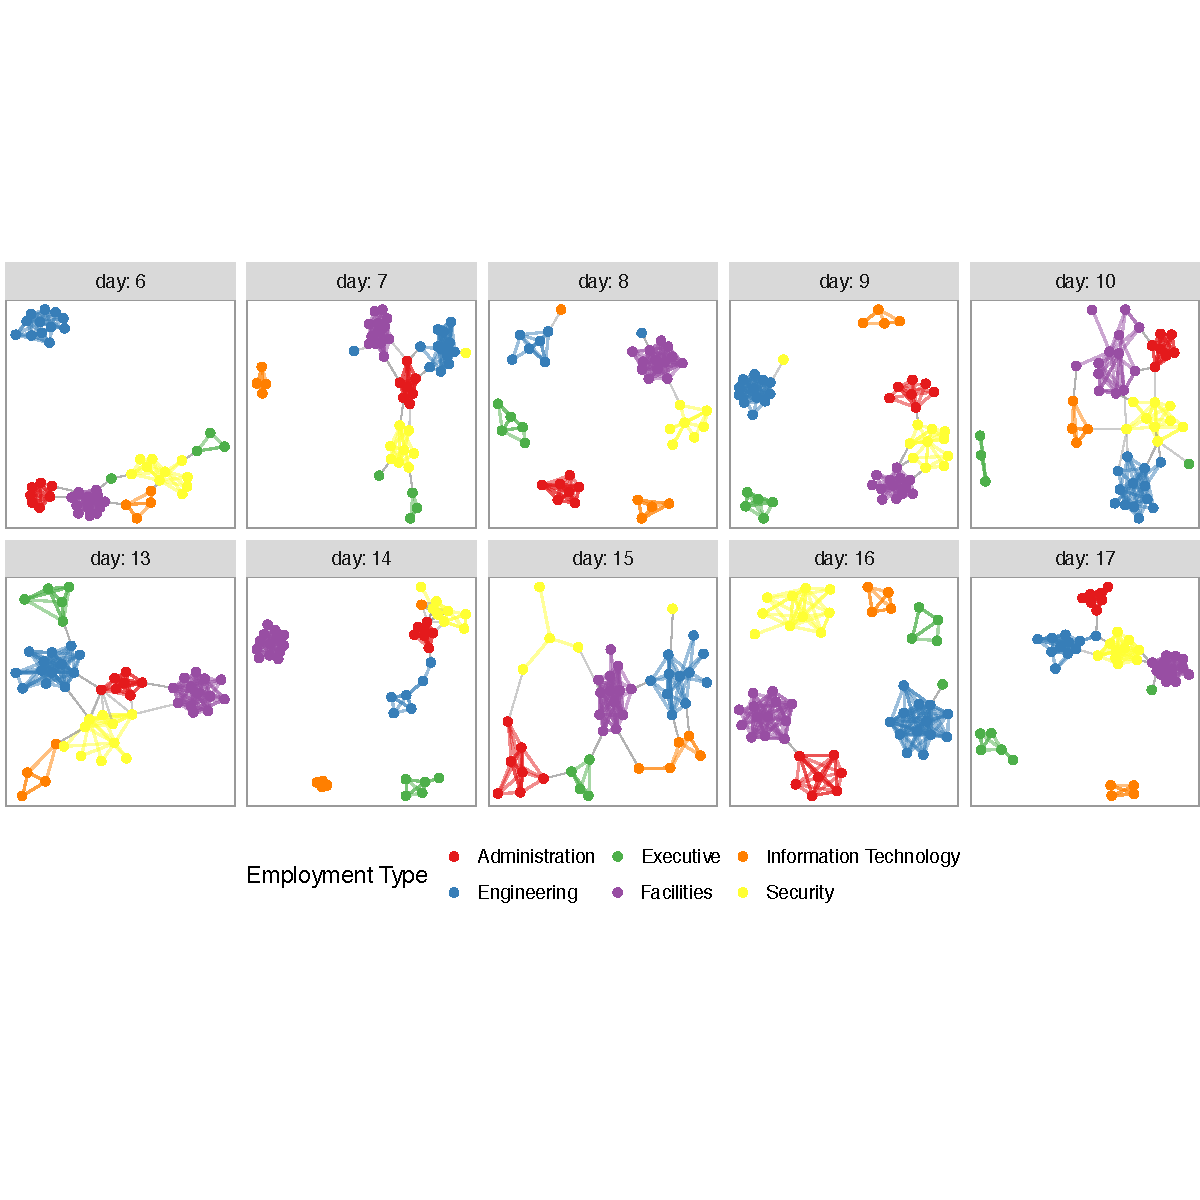
\includegraphics[width=\textwidth]{figure/email_facet_geom_net-1.pdf}
\end{subfigure}
%
\begin{subfigure}[t]{\textwidth}
\caption{ggnetwork}
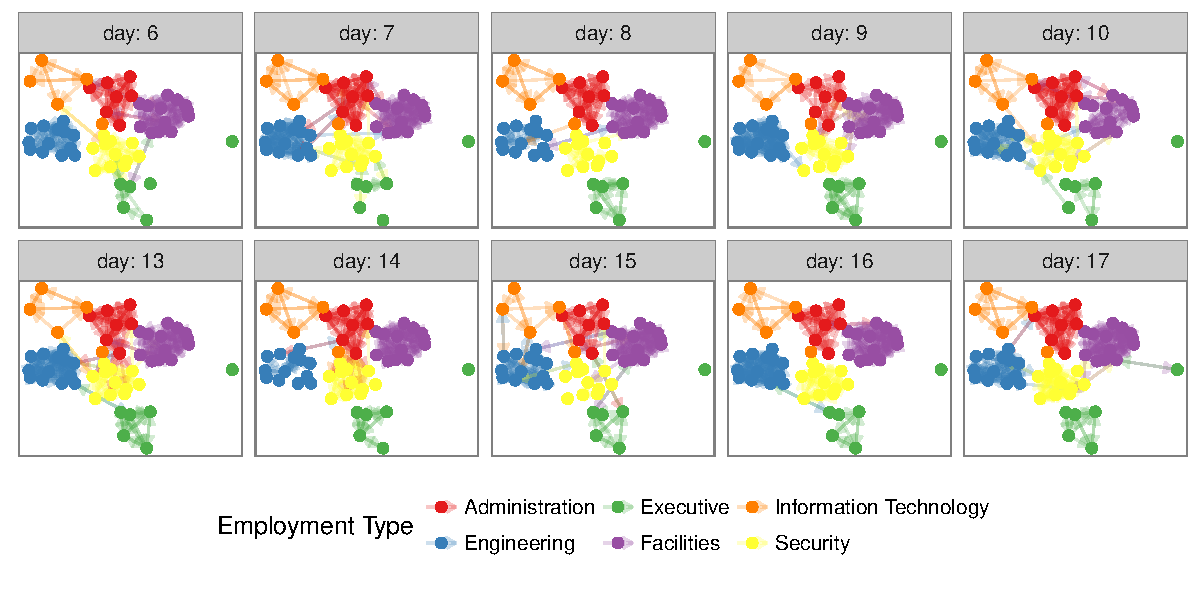
\includegraphics[width=\textwidth]{figure/email_facet_ggnetwork-1.pdf}
\end{subfigure}

\caption{\label{fig:email_facet} The same email network as in figure~\ref{fig.cap:email} facetted by day of the week.}
\end{figure}
\afterpage{\clearpage}
\begin{knitrout}
\definecolor{shadecolor}{rgb}{1, 1, 1}\color{fgcolor}\begin{kframe}
\begin{verbatim}
# ggnet2 code for the email network facetted by day as shown in fig.4a

# data preparation
em.day <- subset(email$edges, nrecipients < 54)[, c("From", "to", "day") ]
em.day <- lapply(unique(em.day$day),
                 function(x) subset(em.day, day == x)[, 1:2 ])
em.day <- lapply(em.day, network, directed = TRUE)
for (i in 1:length(em.day)) {
  em.day[[ i ]] %v% "curr_empl_type" <-
    em.cet[ network.vertex.names(em.day[[ i ]]) ]
  em.day[[ i ]] %n% "day" <- unique(email$edges$day)[ i ]
}

# plot ggnet2
g <- list(length(em.day))
for (i in 1:length(em.day)) {
  g[[ i ]] <- ggnet2(em.day[[ i ]], size = 2, color = "curr_empl_type",
                     palette = "Set1", arrow.size = 0, arrow.gap = 0.01,
                     edge.alpha = 0.1, legend.position = "none") +
    ggtitle(paste("Day", em.day[[ i ]] %n% "day")) +
    theme(panel.border = element_rect(color = "grey50", fill = NA),
          aspect.ratio = 1)
}
gridExtra::grid.arrange(grobs = g, nrow = 2)
\end{verbatim}
\end{kframe}
\end{knitrout}

\begin{knitrout}
\definecolor{shadecolor}{rgb}{1, 1, 1}\color{fgcolor}\begin{kframe}
\begin{verbatim}
# geomnet code for the  email network facetted by day as shown in fig.4b

# data step: making sure that there is one entry for each person on each day
employee <- data.frame(expand.grid(label = unique(email$nodes$label),
                                   day = unique(email$edges$day)))
employee <- merge(employee, email$nodes, by = "label")
emailnet <- merge(subset(email$edges, nrecipients < 54), employee,
                  by.x = c("From", "day"), by.y = c("label", "day"),
                  all = TRUE)

# creating the plot
ggplot(data = emailnet, aes(from_id = From, to_id = to)) +
  geom_net(aes(colour = CurrentEmploymentType,
               group = CurrentEmploymentType,
               linewidth = 2 * (...samegroup.. / 8 + .125)),
           fiteach = TRUE, ealpha = 0.5, size = 1.5) +
  scale_colour_brewer("Employment Type", palette = "Set1") +
  theme_net() +
  facet_wrap(~day, nrow = 2, labeller = "label_both") +
  theme(legend.position = "bottom",
        panel.border = element_rect(fill = NA, colour = "grey60"),
        plot.margin = unit(c(0, 0, 0, 0), "mm"))
\end{verbatim}
\end{kframe}
\end{knitrout}

\begin{knitrout}
\definecolor{shadecolor}{rgb}{1, 1, 1}\color{fgcolor}\begin{kframe}
\begin{verbatim}
# ggnetwork code for the  email network facetted by day as shown in fig.4c

# create the network and aesthetics
edges <- subset(email$edges, nrecipients < 54)
edges <- edges[, c("From", "to", "day") ]
em.net <- network(edges[, 1:2])
set.edge.attribute(em.net, "day", edges[, 3])
em.net %v% "curr_empl_type" <- em.cet[ network.vertex.names(em.net) ]

# create the plot
ggplot(ggnetwork(em.net, arrow.gap = 0.02, by = "day"),
       aes(x, y, xend = xend, yend = yend)) +
  geom_edges(
    aes(color = curr_empl_type),
    alpha = 0.25,
    arrow = arrow(length = unit(5, "pt"),
                  type = "closed")) +
  geom_nodes(aes(color = curr_empl_type),
             size = 2) +
  scale_color_brewer("Employment Type",
                     palette = "Set1") +
  facet_wrap(~day, nrow = 2, labeller = "label_both") +
  theme_facet(legend.position = "bottom")
\end{verbatim}
\end{kframe}
\end{knitrout}

Note that the main difference in the visualizations of Figure~\ref{fig:email_facet} stems from whether \emph{one} layout is used across all panels (as for the \code{ggnetwork} example) or whether individual layouts are fit to each of the subsets (as for the \code{ggnet2} and the \code{geomnet} examples). In \code{geomnet} this is controlled via the argument \code{fiteach}. By default  \code{fiteach = TRUE}, but \code{fiteach = FALSE} results in all panels sharing the same layout. Through the facetting it becomes obvious that there are several days where one or more of the departments does not communicate with any of the other departments. There are only two days, day 13 and day 15, without any isolated department communications. Facetting is one of the major benefits of implementing tools for network visualization in \pkg{ggplot2}. Facetting allows the user to quickly separate dense networks into smaller subnetworks for easy visual comparison and analyses, a feature that the other network visualization tools do not have.

\subsection{\pkg{ggplot2} theme elements} % ====================================

This example comes from the \code{theme()} help page in the \pkg{ggplot2} documentation \citep{ggplot2}.  It is a directed network which shows the structure of the inheritance of theme options in the construction of a \pkg{ggplot2} plot. There are 53 vertices and 36 edges in this network. Each vertex represents one possible theme option. There is an arrow from one theme option to another if the element represented by the `to' vertex inherits its values from the `from' vertex.  For example, the \code{axis.ticks.x} option inherits its value from the \code{axis.ticks} value, which in turn inherits its value from the \code{line} option.  Thus, setting the \code{line} option to a value such as \code{element\_blank()} sets the entire inheritance tree to \code{element\_blank()}, and no lines appear anywhere on the plot background. %%% SCT: I removed this sentence because it's not true for all of our functions. %Finally, note that the vertices without edges were incorporated into the plot by adding their labels to the edges data frame in both the  \code{from\_id} and \code{to\_id} columns. %before passing the edges data frame to \code{ggplot}.

\begin{figure}[hbtp]
\begin{subfigure}[t]{\textwidth}
\caption{ggnet2}
\vspace{1em}

             \begin{adjustbox}{valign=t}

             \begin{minipage}{.49\textwidth}
 \begin{knitrout}\footnotesize
\definecolor{shadecolor}{rgb}{1, 1, 1}\color{fgcolor}\begin{kframe}
\begin{verbatim}
te.net <- network(theme_elements$edges)
te.net %v% "size" <-
  sqrt(10 * (sna::degree(te.net) + 1))

ggnet2(te.net, label = TRUE, color = "white",
       label.size = "size", layout.exp = 0.15)
\end{verbatim}
\end{kframe}
\end{knitrout} \vspace{1em}

                   \end{minipage}

                  \begin{minipage}{.49\textwidth}

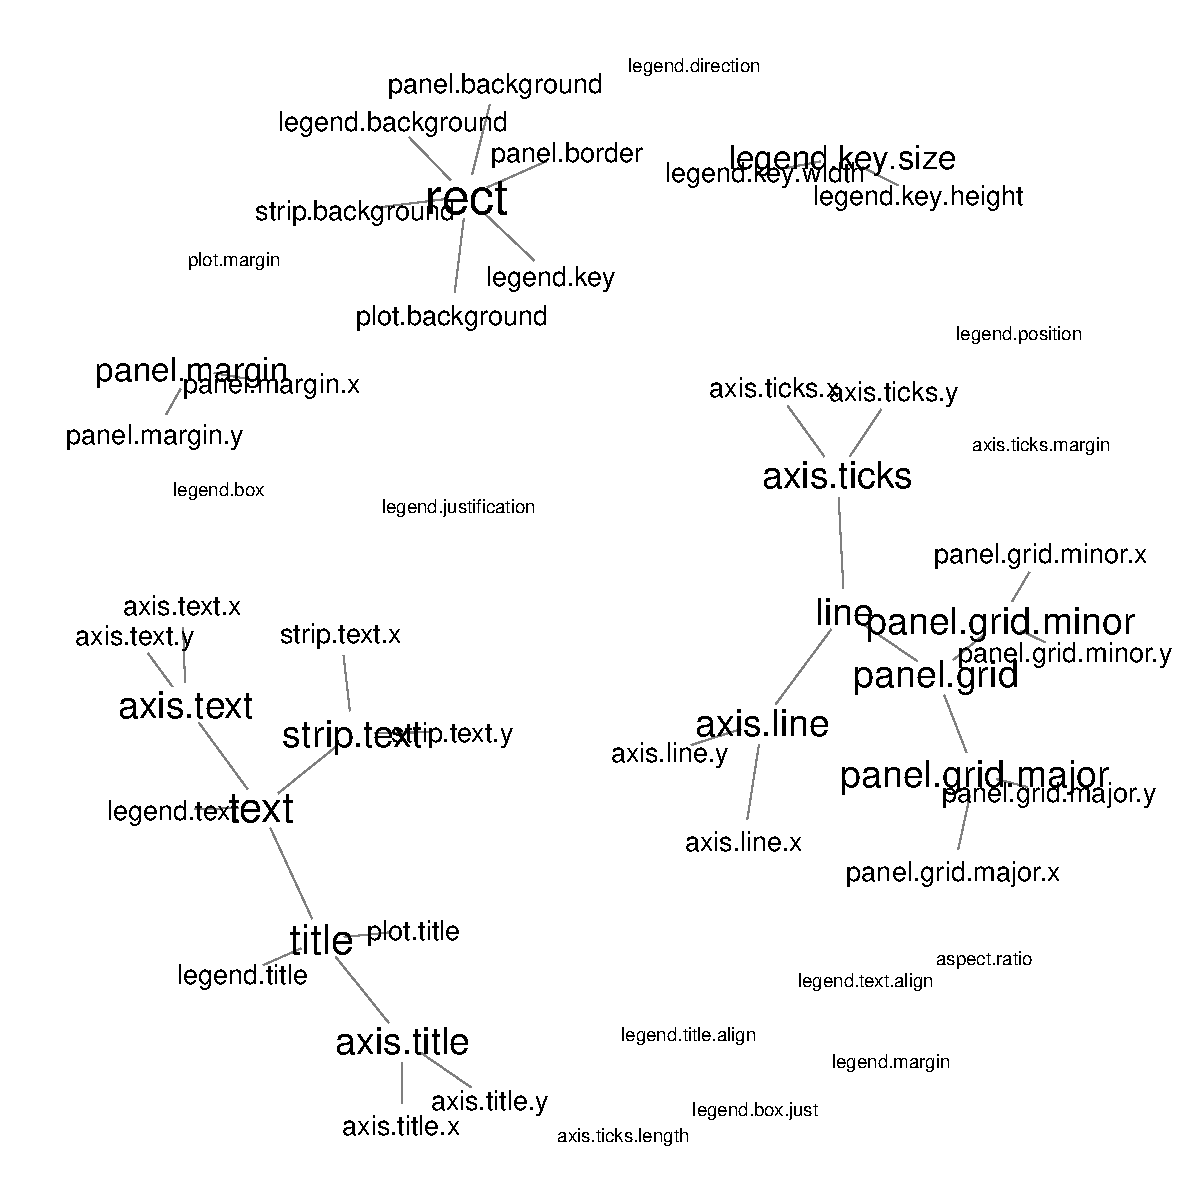
\includegraphics[width=\textwidth]{figure/theme_ggnet2-1.pdf}

                          \end{minipage}

                          \end{adjustbox}
\end{subfigure}
%
\begin{subfigure}[t]{\textwidth}
\caption{geomnet}
\vspace{1em}

             \begin{adjustbox}{valign=t}

             \begin{minipage}{.49\textwidth}
 \begin{knitrout}\footnotesize
\definecolor{shadecolor}{rgb}{1, 1, 1}\color{fgcolor}\begin{kframe}
\begin{verbatim}
# data step: merge nodes and edges and
# introduce a degree-out variable
TEnet <- merge(
  theme_elements$edges,
  theme_elements$vertices,
  by.x = "parent", by.y = "name", all = TRUE)
TEnet <- TEnet %>%
  group_by(parent) %>%
  mutate(degree = sqrt(10 * n() + 1))

# create plot:
ggplot(data = TEnet,
       aes(from_id = parent, to_id = child)) +
  geom_net(
    aes(fontsize = degree), directed = TRUE,
    label = TRUE, vjust = -.5, size = 3,
    ecolour = "grey70", arrowsize = 0.5,
    linewidth = 0.5) +
  theme_net() +
  xlim(c(-0.05, 1.05))
\end{verbatim}
\end{kframe}
\end{knitrout} \vspace{1em}

                   \end{minipage}

                  \begin{minipage}{.49\textwidth}

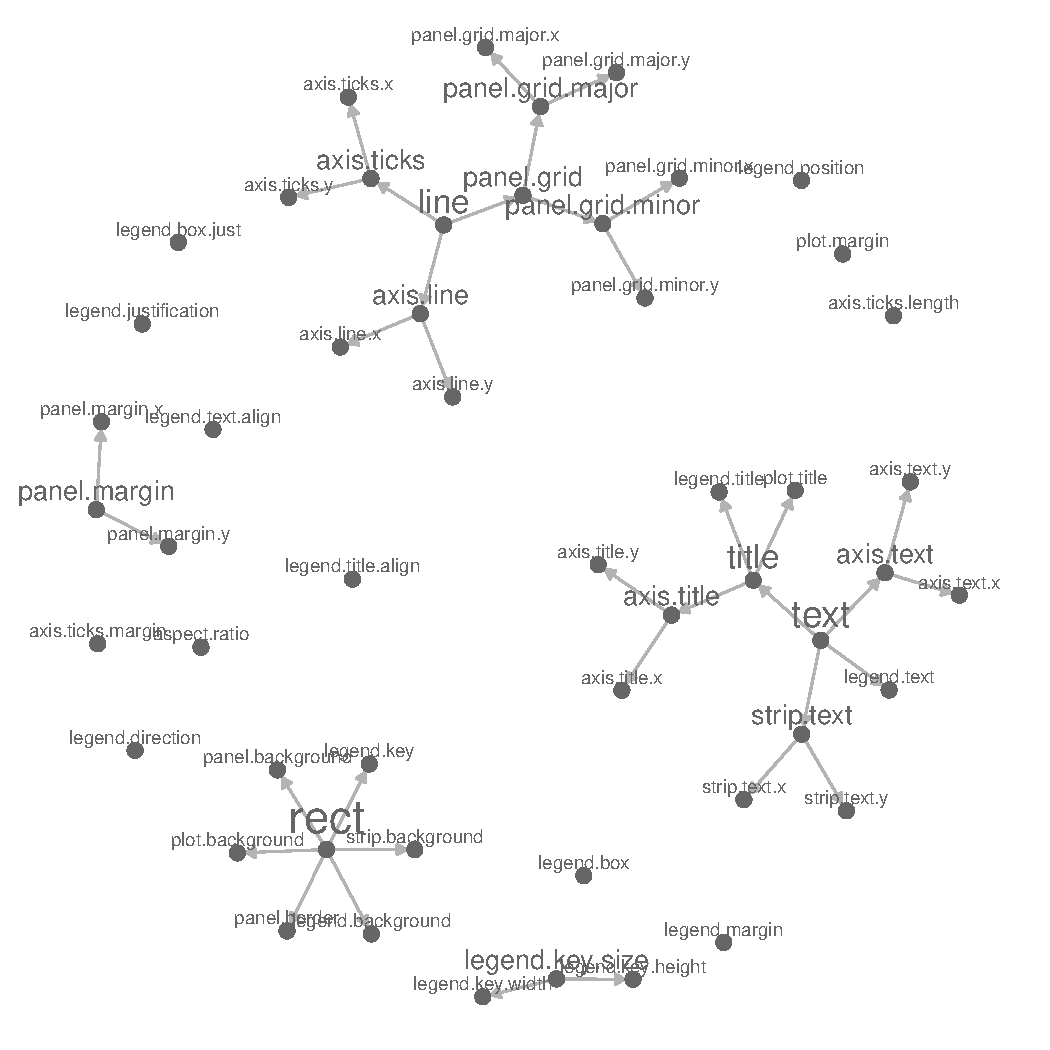
\includegraphics[width=\textwidth]{figure/theme_geom_net-1.pdf}

                          \end{minipage}

                          \end{adjustbox}
\end{subfigure}
%
\begin{subfigure}[t]{\textwidth}
\caption{ggnet2}
\vspace{1em}

             \begin{adjustbox}{valign=t}

             \begin{minipage}{.49\textwidth}
 \begin{knitrout}\footnotesize
\definecolor{shadecolor}{rgb}{1, 1, 1}\color{fgcolor}\begin{kframe}
\begin{verbatim}
ggplot(ggnetwork(te.net),
       aes(x, y, xend = xend, yend = yend)) +
  geom_edges() +
  geom_nodes(size = 12, color = "white") +
  geom_nodetext(
    aes(size = size, label = vertex.names)) +
  scale_size_continuous(range = c(4, 8)) +
  guides(size = FALSE) +
  theme_blank()
\end{verbatim}
\end{kframe}
\end{knitrout} \vspace{1em}

                   \end{minipage}

                  \begin{minipage}{.49\textwidth}

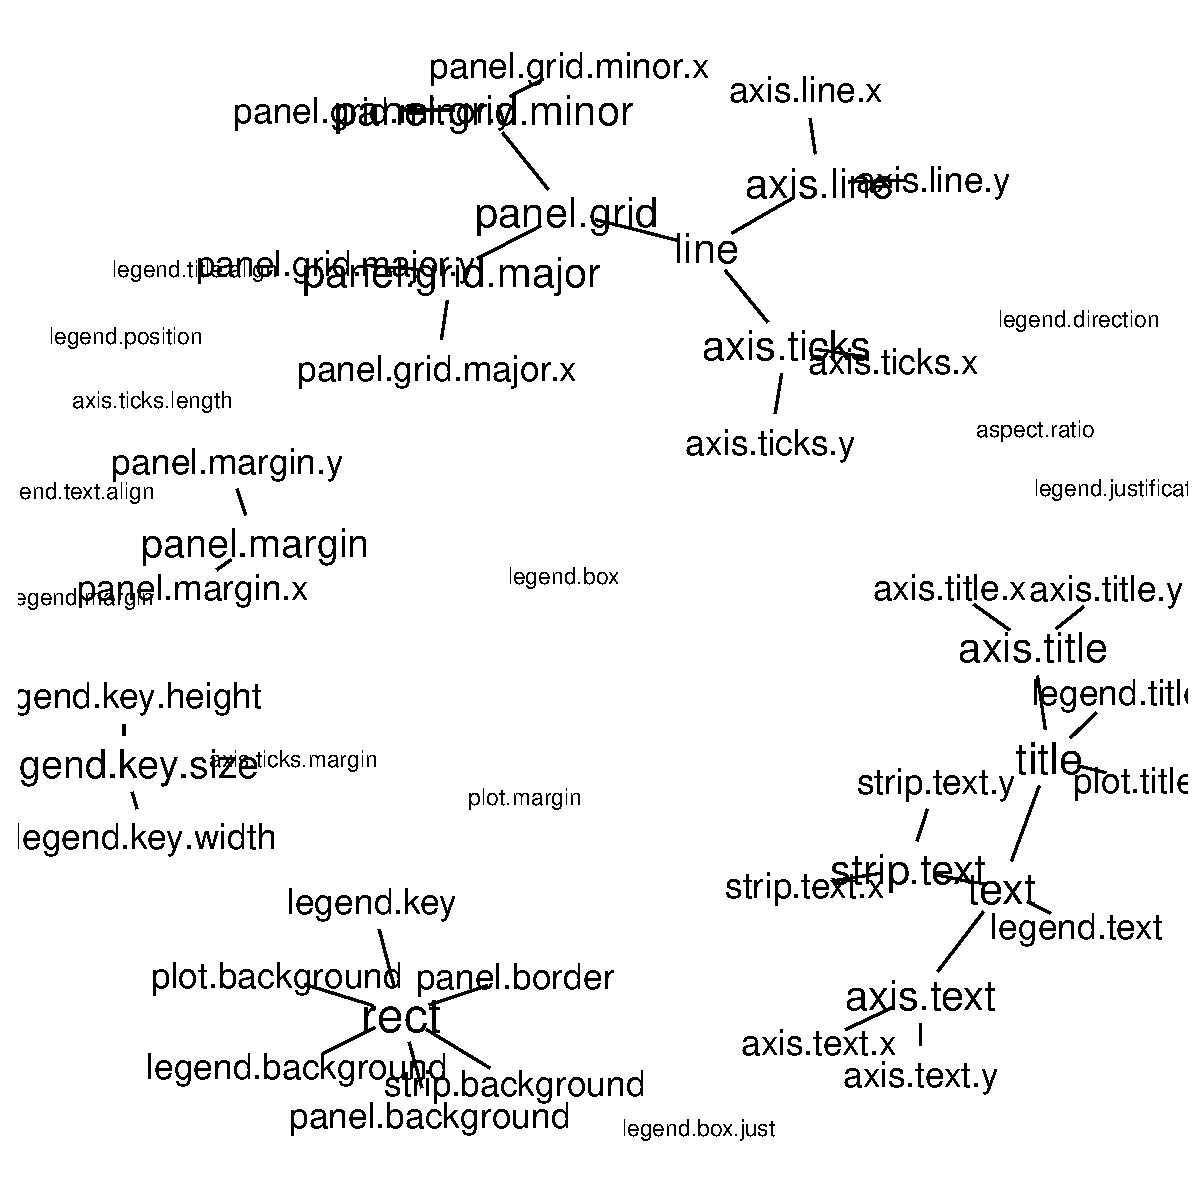
\includegraphics[width=\textwidth]{figure/theme_ggnetwork-1.pdf}

                          \end{minipage}

                          \end{adjustbox}
\end{subfigure}

\caption{\label{fig.cap:theme} Inheritance structure of \pkg{ggplot2} theme elements. This is a recreation of the graph found at \protect\url{http://docs.ggplot2.org/current/theme.html}.}
\end{figure}
\afterpage{\clearpage}

The inheritance structure is plotted in figure \ref{fig.cap:theme}.  In these plots, it is easy to quickly determine the parent and child vertices. The parents with the most children are the \code{rect}, \code{text}, and \code{line} elements, so we made their labels larger in order to emphasize their importance. In each case, the label size is a function of the out degree of the vertices.
%Using this plot made creation of the \code{theme\_net} object used throughout these examples very simple. We just made set each of the major parent elements, \code{text}, \code{rect}, and \code{line} to \code{element\_blank()} and then set the aspect ratio equal to one.

\subsection{Romantic relationships in \emph{Mad Men}} % ========================

  The following code creates the network example given in Figure~\ref{fig.cap:madmen} in the introduction. We changed the vertex size and edge color for all vertices and edges, included vertex labels, and colored the vertices according to the character's gender.

The code for the other two approaches follows below and the corresponding networks are shown in figure~\ref{fig:madmen-2}.

\begin{knitrout}
\definecolor{shadecolor}{rgb}{1, 1, 1}\color{fgcolor}\begin{kframe}
\begin{verbatim}
# data step for both ggnet2 and ggnetwork
# create undirected network
mm.net <- network(madmen$edges[, 1:2], directed = FALSE)
# gender vertex attribute
rownames(madmen$vertices) <- madmen$vertices$label
mm.net %v% "gender" <- as.character(
  madmen$vertices[ network.vertex.names(mm.net), "Gender"]
)
# gender color palette
mm.col <- c("female" = "#ff69b4", "male" = "#0099ff")
\end{verbatim}
\end{kframe}
\end{knitrout}

\begin{knitrout}
\definecolor{shadecolor}{rgb}{1, 1, 1}\color{fgcolor}\begin{kframe}
\begin{verbatim}
ggnet2(mm.net, color = mm.col[ mm.net %v% "gender" ],
       label = TRUE, label.color = mm.col[ mm.net %v% "gender" ],
       size = 4, vjust = -0.6)
\end{verbatim}
\end{kframe}
\end{knitrout}

\begin{knitrout}
\definecolor{shadecolor}{rgb}{1, 1, 1}\color{fgcolor}\begin{kframe}
\begin{verbatim}
ggplot(data = ggnetwork(mm.net), aes(x, y, xend = xend, yend = yend)) +
  geom_edges(color = "grey50") +
  geom_nodes(aes(colour = gender), size = 4) +
  geom_nodetext(aes(colour = gender, label = vertex.names),
                size = 4, vjust = -0.6) +
  scale_colour_manual(values = mm.col) +
  xlim(c(-0.05, 1.05)) +
  theme_blank() +
  theme(legend.position = "bottom")
\end{verbatim}
\end{kframe}
\end{knitrout}

\begin{figure}[hbtp]
\begin{subfigure}[t]{.495\textwidth}
\caption{ggnet2}
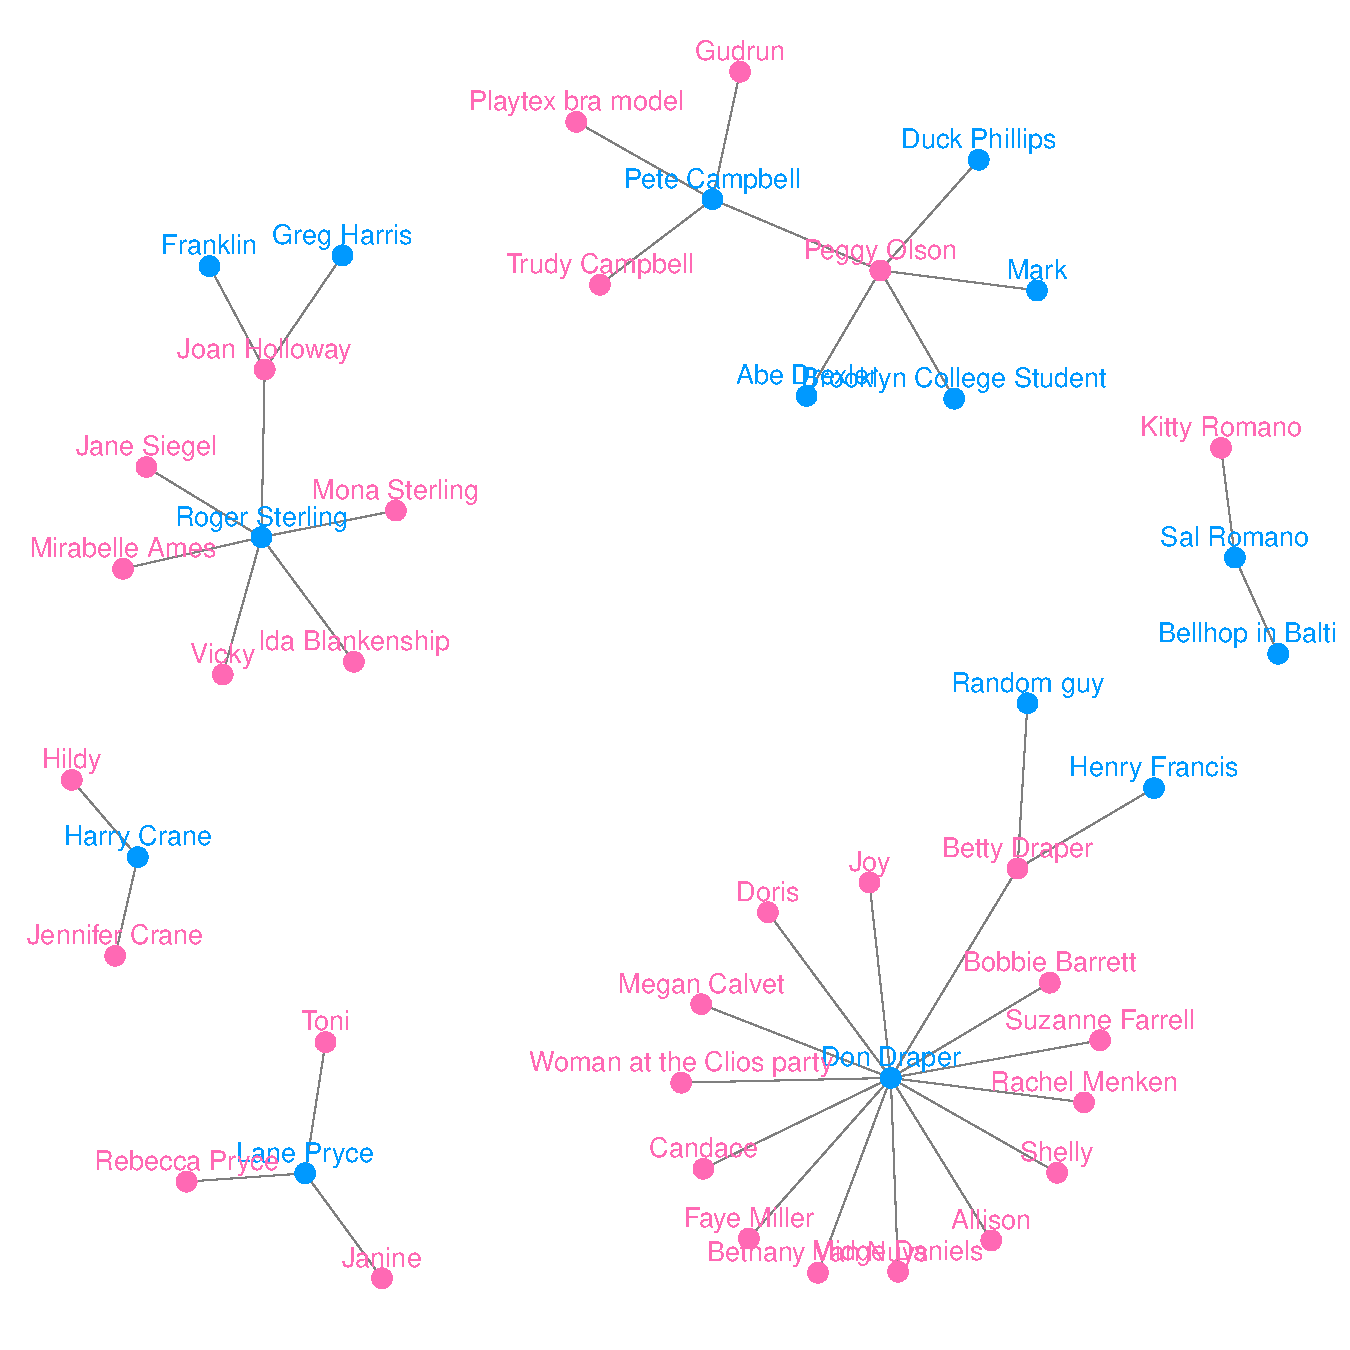
\includegraphics[width=\textwidth]{figure/madmen_ggnet2-1.pdf}
\end{subfigure}
\begin{subfigure}[t]{.495\textwidth}
\caption{ggnetwork}
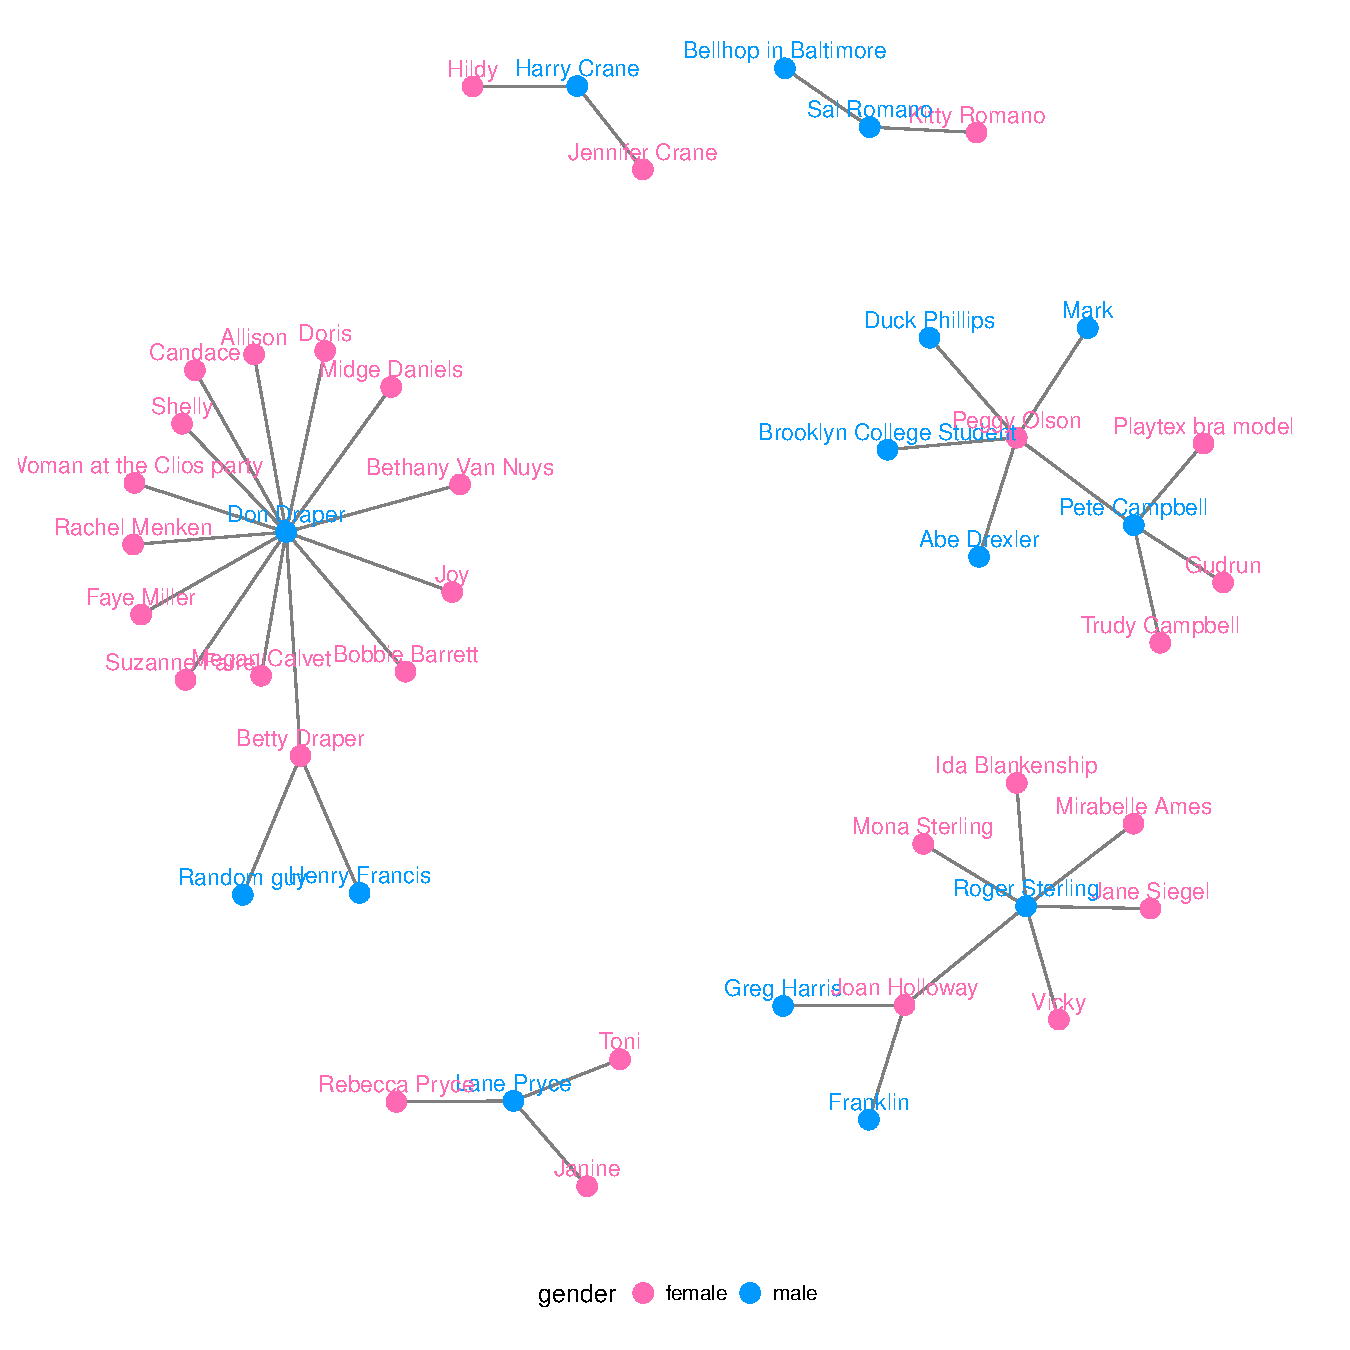
\includegraphics[width=\textwidth]{figure/madmen_ggnetwork-1.pdf}
\end{subfigure}

\caption{\label{fig:madmen-2} Graph of the characters in the show Mad Men who are linked by a romantic relationship, ggnet2 and ggnetwork implementation.}
\end{figure}
%\afterpage{\clearpage}

 There is another Mad Men network given in the \pkg{gcookbook} package \citep{madmen}. It is a directed network, also of romantic relationships between characters, but it additionally includes all advances made by one character that were rejected by the other.  For example, Roger Sterling made advances toward Betty Draper, but Betty refused him,  so there is a directed edge going from Roger to Betty, but not from Betty to Roger.  If the advance is reciprocated, such as between Sal Romano and the Bellhop, there are two directed edges between the two vertices.

\begin{figure}
\begin{knitrout}
\definecolor{shadecolor}{rgb}{1, 1, 1}\color{fgcolor}\begin{kframe}
\begin{verbatim}
# data step for ggnet2 and ggnetwork
# create directed network
mm.dir <- network(mm.directed$edges, directed = TRUE)
# gender vertex attribute
rownames(mm.directed$vertices) <- mm.directed$vertices$label
mm.dir %v% "gender" <- as.character(
  mm.directed$vertices[ network.vertex.names(mm.dir), "Gender" ]
)
\end{verbatim}
\end{kframe}
\end{knitrout}
\caption{\label{mm2:datastep} Data preparation for the directed network of the  Mad Men example in Figures~\ref{mm2:ggnet2} and~\ref{mm2:ggnetwork}.}

\end{figure}
\begin{figure}[hbtp]
\begin{subfigure}[t]{\textwidth}
\caption{ggnet2\label{mm2:ggnet2}}
\vspace{1em}

             \begin{adjustbox}{valign=t}

             \begin{minipage}{.49\textwidth}
 \begin{knitrout}\footnotesize
\definecolor{shadecolor}{rgb}{1, 1, 1}\color{fgcolor}\begin{kframe}
\begin{verbatim}
# see fig.7 for data preparation

ggnet2(
  mm.dir, mode = "fruchtermanreingold", size = 3,
  color = mm.col[ mm.dir %v% "gender" ],
  label = TRUE,
  label.color = mm.col[ mm.dir %v% "gender" ],
  hjust = -0.1, legend.position = "bottom",
  layout.exp = 0.15, arrow.size = 7.5,
  arrow.gap = 0.02
)
\end{verbatim}
\end{kframe}
\end{knitrout} \vspace{1em}

                   \end{minipage}

                  \begin{minipage}{.49\textwidth}

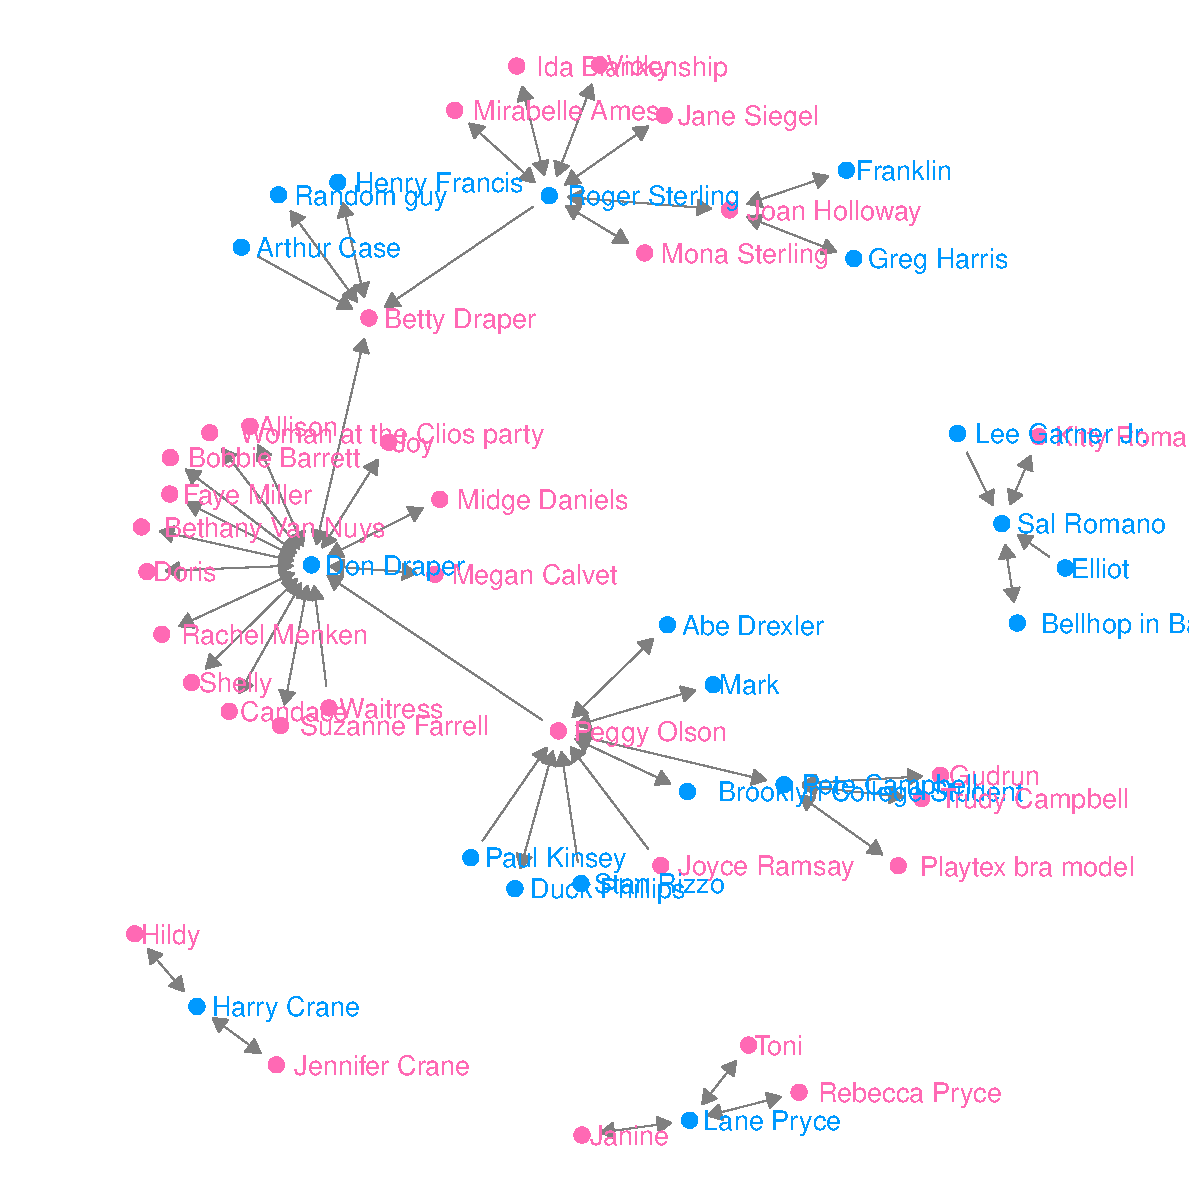
\includegraphics[width=\textwidth]{figure/madmen2_ggnet2-1.pdf}

                          \end{minipage}

                          \end{adjustbox}
\end{subfigure}
%
\begin{subfigure}[t]{\textwidth}
\caption{geomnet}
\vspace{1em}

             \begin{adjustbox}{valign=t}

             \begin{minipage}{.49\textwidth}
 \begin{knitrout}\footnotesize
\definecolor{shadecolor}{rgb}{1, 1, 1}\color{fgcolor}\begin{kframe}
\begin{verbatim}
MM2net <- merge(
  mm.directed$edges,
  mm.directed$vertices,
  by.x = "Name1", by.y = "label", all = TRUE)

ggplot(data = MM2net,
       aes(from_id = Name1, to_id = Name2)) +
  geom_net(
    aes(colour = Gender),  directed = TRUE,
    label = TRUE, ecolour = "grey50",
    linewidth = 0.5, size = 2.5, vjust = -.5,
    layout = "fruchtermanreingold") +
  scale_colour_manual(
    values = c("#ff69b4", "#0099ff")) +
  xlim(c(-0.1, 1.1)) +
   theme_net() +
  theme(legend.position = "bottom")
\end{verbatim}
\end{kframe}
\end{knitrout} \vspace{1em}

                   \end{minipage}

                  \begin{minipage}{.49\textwidth}

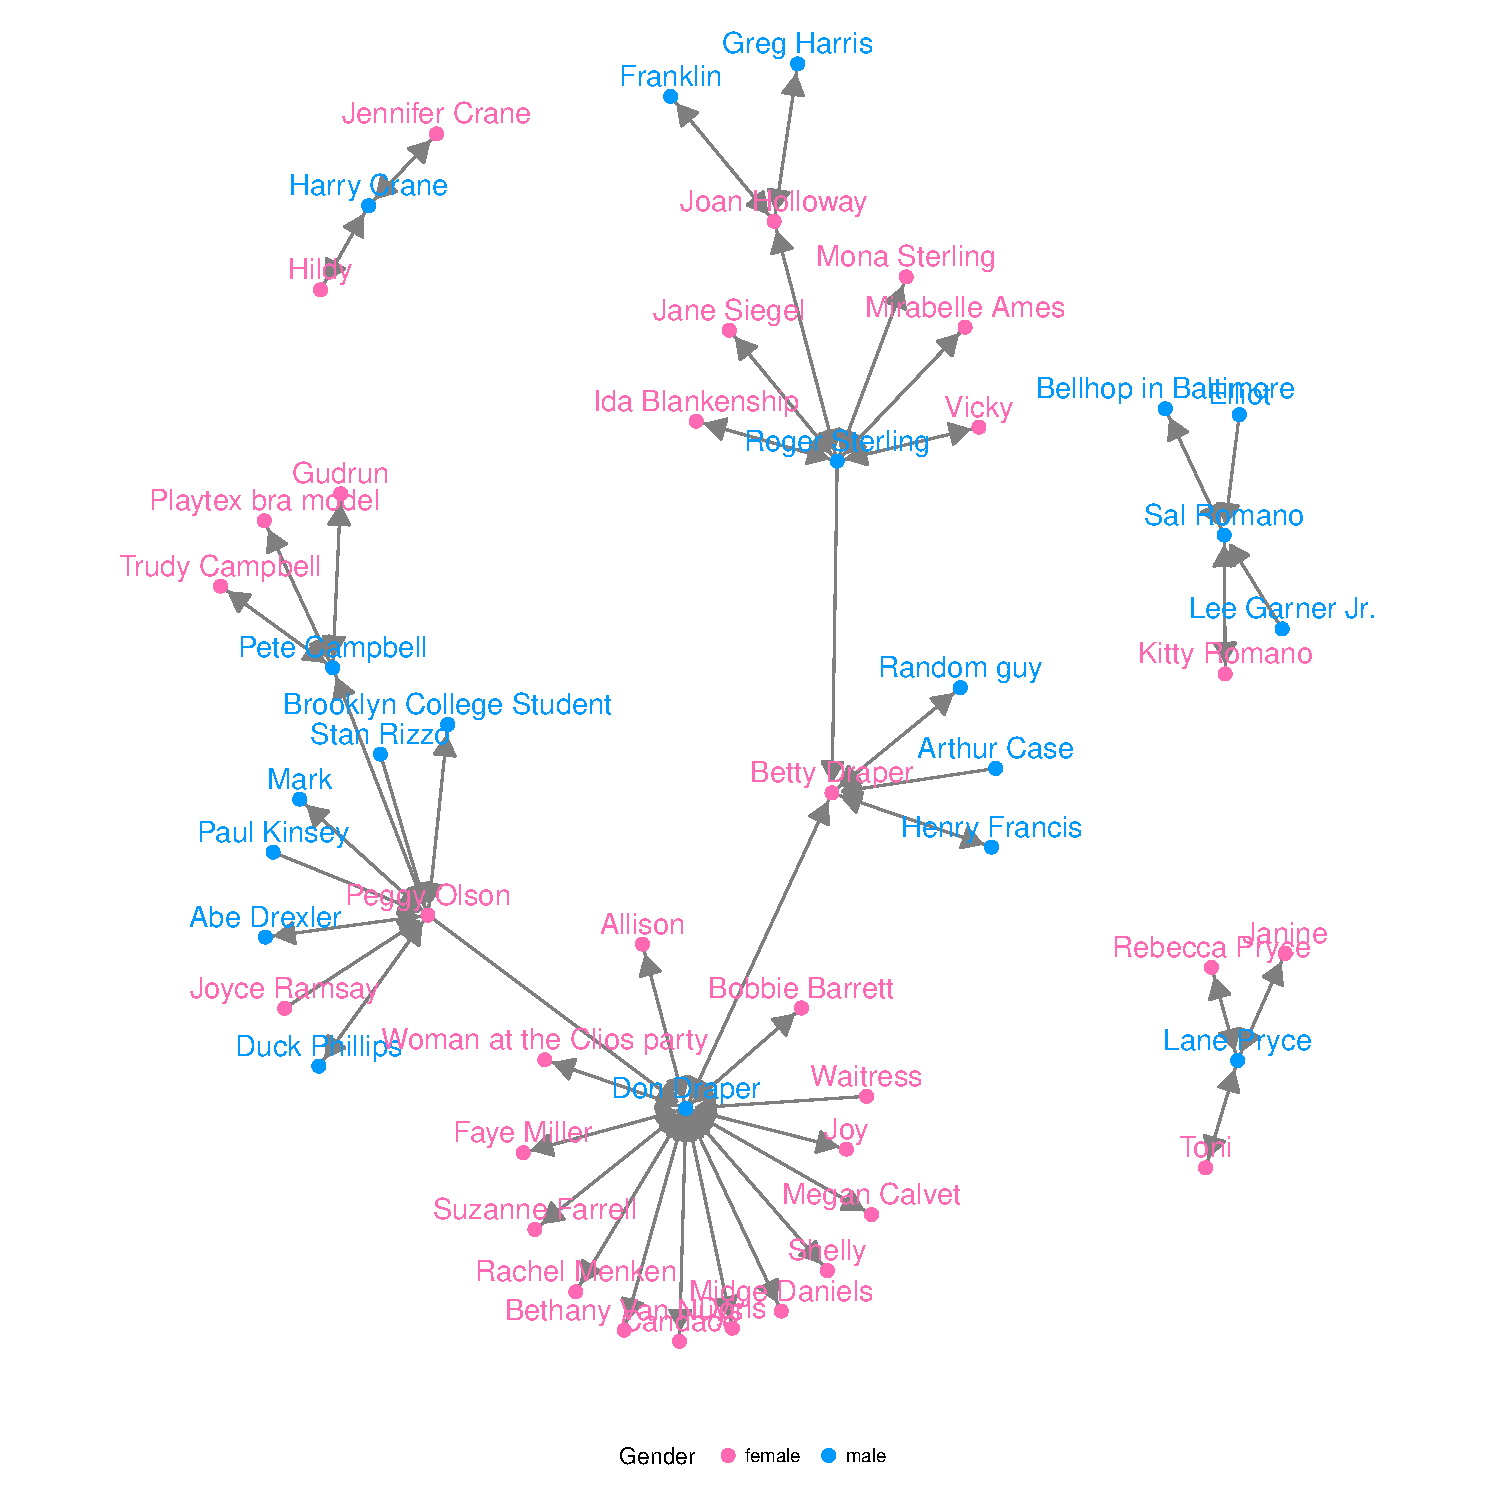
\includegraphics[width=\textwidth]{figure/madmen2_geom_net-1.pdf}

                          \end{minipage}

                          \end{adjustbox}
\end{subfigure}
%
\begin{subfigure}[t]{\textwidth}
\caption{ggnetwork \label{mm2:ggnetwork}}
\vspace{1em}

             \begin{adjustbox}{valign=t}

             \begin{minipage}{.49\textwidth}
 \begin{knitrout}\footnotesize
\definecolor{shadecolor}{rgb}{1, 1, 1}\color{fgcolor}\begin{kframe}
\begin{verbatim}
# see fig.7 for data preparation

ggplot(
  ggnetwork(mm.dir,
            layout = "fruchtermanreingold"),
       aes(x, y, xend = xend, yend = yend)) +
  geom_edges(
    color = "grey50",
    arrow = arrow(length = unit(10, "pt"),
                  type = "closed")) +
  geom_nodes(size = 3, aes(color = gender)) +
  geom_nodetext(aes(label = vertex.names,
                    color = gender),
                hjust = -0.1) +
  scale_color_manual(values = mm.col) +
  theme_blank() +
  theme(legend.position = "bottom")
\end{verbatim}
\end{kframe}
\end{knitrout} \vspace{1em}

                   \end{minipage}

                  \begin{minipage}{.49\textwidth}

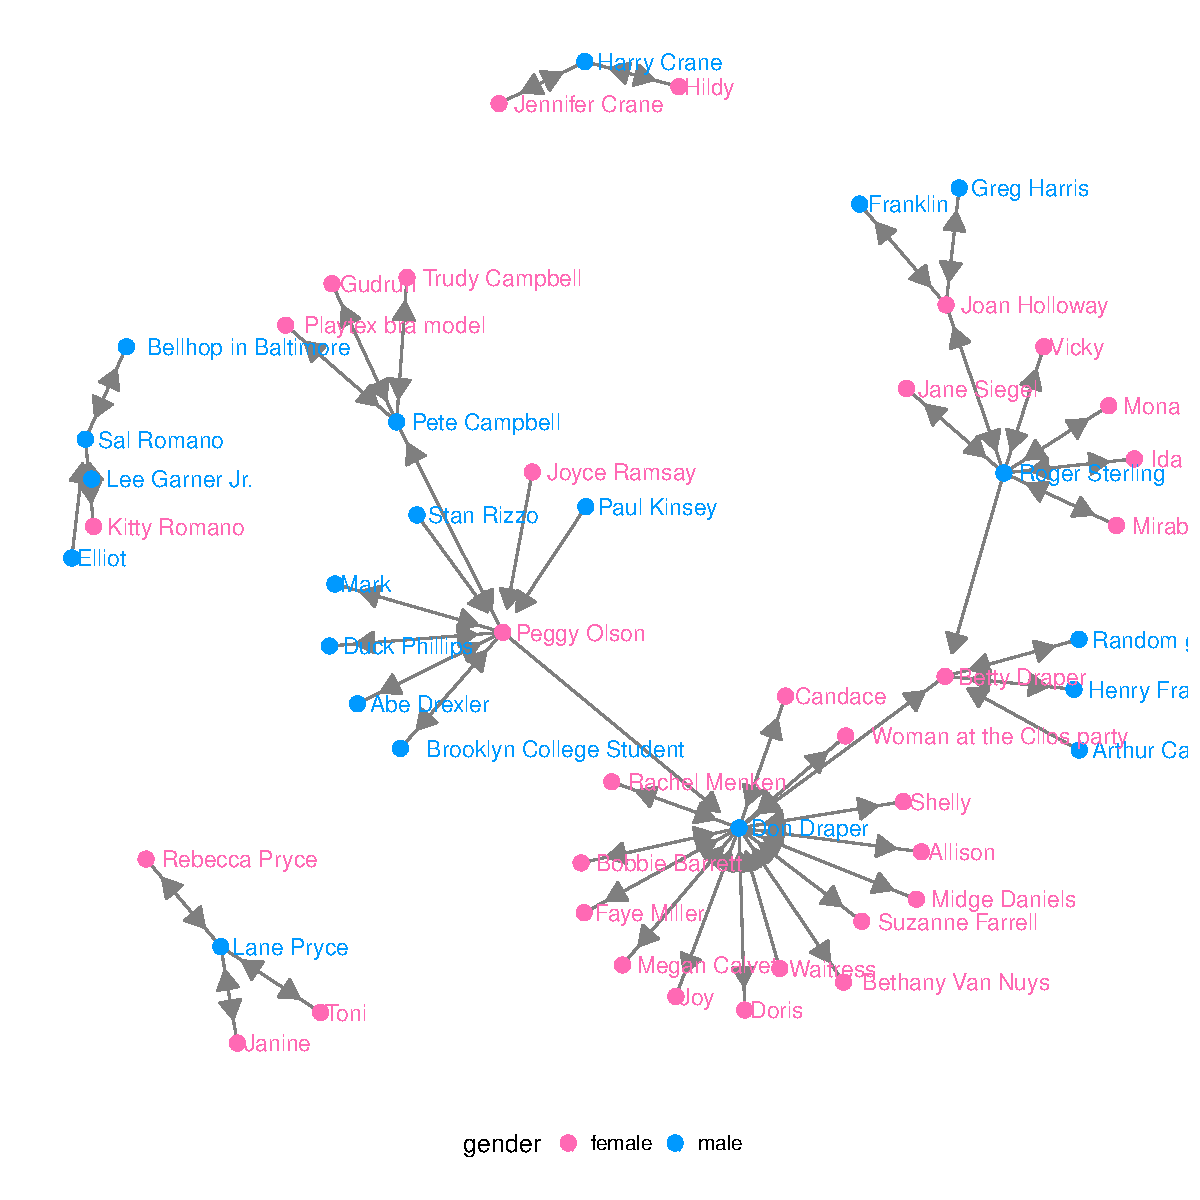
\includegraphics[width=\textwidth]{figure/madmen2_ggnetwork-1.pdf}

                          \end{minipage}

                          \end{adjustbox}
\end{subfigure}
\caption{\label{fig.cap:madmen2} A directed network of relationships in Mad Men.}
\end{figure}
\afterpage{\clearpage}

This network is shown in figure \ref{fig.cap:madmen2}.  It is much more densely connected than the previous Mad Men example.  This network allows us to see more of the drama in the show. For instance, we can see that Roger made advances towards Betty, his business partner's wife, which is much more scandalous than what appears in the first network.

\subsection{College football} % ================================================

This next example comes from M.E.J. Newman's network data web page \citep{football}.  It is an undirected network consisting of all regular season college football games played between Division I schools in Fall of 2000.  There are 115 vertices and 613 edges: each vertex represents a school, and an edge represents a game played between two schools. There is an additional variable in the vertex data frame corresponding to the conference each team belongs to, and there is an additional variable in the edge data frame that is equal to one if the game occured between teams in the same conference or zero if the game occured between teams in different conferences.

The network of football games is given in figure \ref{fig.cap:football}. Here, we have changed the \code{linetype} aesthetic to correspond to games that occur between teams in the same conference or different conferences.  These lines are dotted and solid, respectively. We have also assigned a different color to each conference, so that the vertices and their labels are colored according to their conference. Additionally, in the first two implementations, the edges between two teams in the same conference share that conference color, while edges between teams in different conferences are a default gray color. This coloring and changing of the linetypes make the structure of the game network easier to view.  There is one conference consisting of Navy, Notre Dame, Utah State, Central Florida, and Connecticut, which is spread out, whereas most other conferences' teams are all very close to each other because they play within conference much more than they play out of conference.  At the time, these five schools were all independents and did not have a home conference.  Without the coloring capability, we would not have been able to pick out that difference as easily.

\begin{figure}[hbtp]
\begin{subfigure}[t]{\textwidth}
\caption{ggnet2}\vspace{-.5cm}
\vspace{1em}

             \begin{adjustbox}{valign=t}

             \begin{minipage}{.49\textwidth}
 \begin{knitrout}\footnotesize
\definecolor{shadecolor}{rgb}{1, 1, 1}\color{fgcolor}\begin{kframe}
\begin{verbatim}
rownames(football$vertices) <-
  football$vertices$label

fb.net <- network(football$edges[, 1:2],
                  directed = FALSE)
set.edge.attribute(
  fb.net, "same.conf",
  football$edges$same.conf)
fb.net %v% "conf" <-
  football$vertices[
    network.vertex.names(fb.net), "value"
    ]

ggnet2(fb.net, mode = "fruchtermanreingold",
       color = "conf",  palette = "Paired",
       color.legend = "Conference",
       edge.color = c("color", "grey75"))
\end{verbatim}
\end{kframe}
\end{knitrout} \vspace{1em}

                   \end{minipage}

                  \begin{minipage}{.49\textwidth}

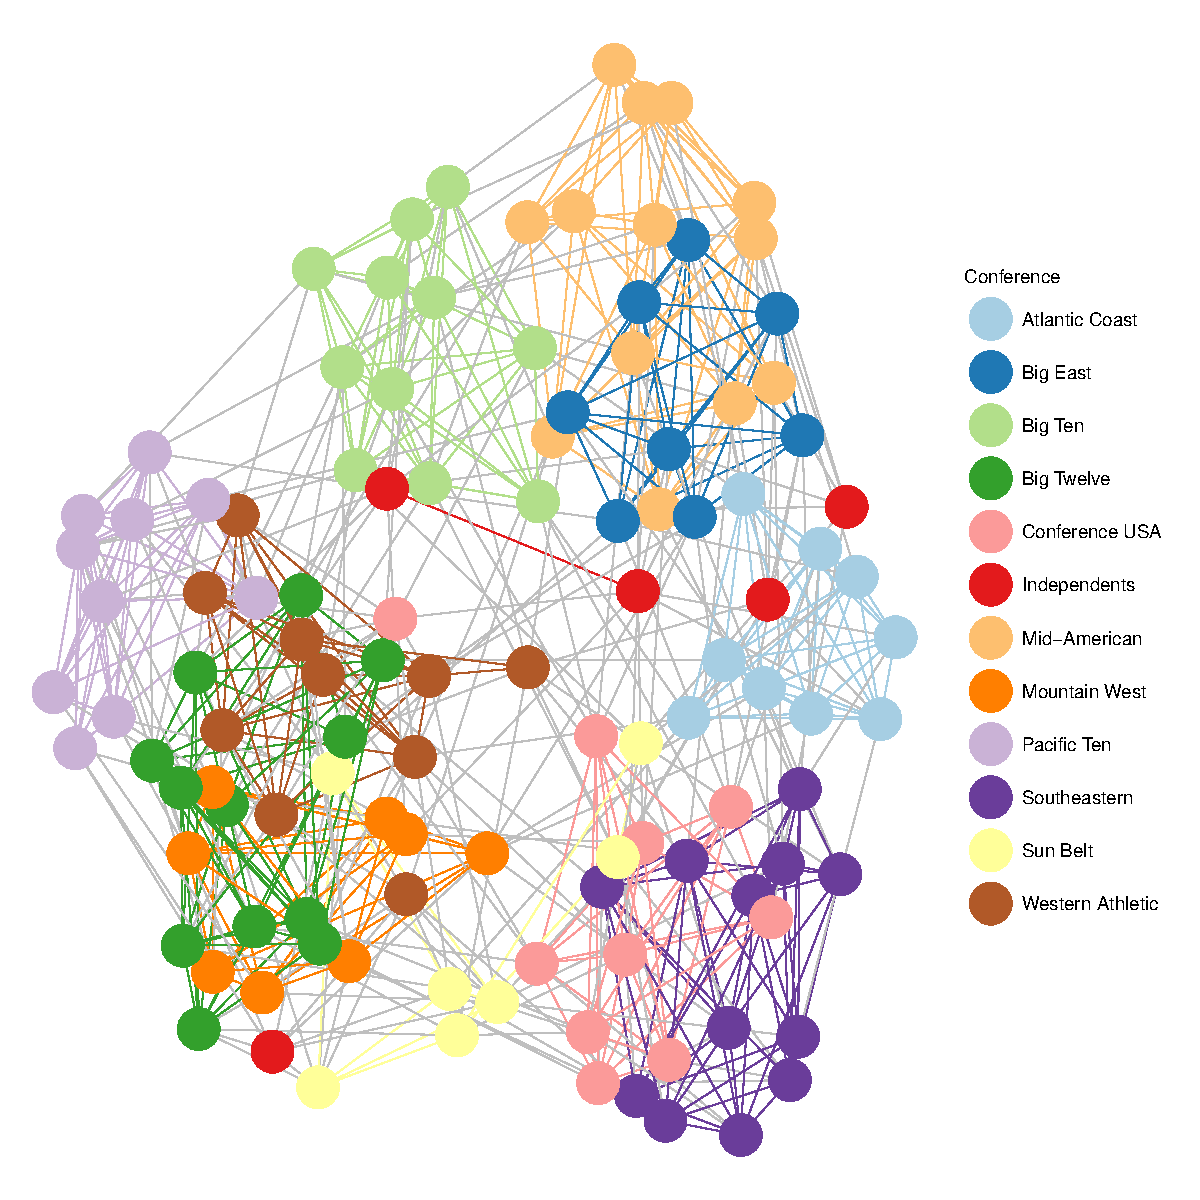
\includegraphics[width=\textwidth]{figure/football_ggnet2-1.pdf}

                          \end{minipage}

                          \end{adjustbox}
\end{subfigure}
%
\begin{subfigure}[t]{\textwidth}
\caption{geomnet}\vspace{-.5cm}
\vspace{1em}

             \begin{adjustbox}{valign=t}

             \begin{minipage}{.49\textwidth}
 \begin{knitrout}\footnotesize
\definecolor{shadecolor}{rgb}{1, 1, 1}\color{fgcolor}\begin{kframe}
\begin{verbatim}
# data step: merge vertices and edges
ftnet <- merge(
  football$edges, football$vertices,
  by.x = "from", by.y = "label", all = TRUE)

# label independent schools
ftnet$schools <- ifelse(
  ftnet$value == "Independents", ftnet$from, "")

# create data plot
ggplot(data = ftnet,
       aes(from_id = from, to_id = to)) +
  geom_net(
    aes(colour = value, group = value,
        linetype = factor(same.conf != 1),
        label = schools),
    linewidth = 0.5,
    size = 5, vjust = -0.75, alpha = 0.3,
    layout = 'fruchtermanreingold') +
  theme_net() +
  theme(legend.position = "bottom") +
  scale_colour_brewer("Conference", palette = "Paired")  +
  guides(linetype = FALSE)
\end{verbatim}
\end{kframe}
\end{knitrout} \vspace{1em}

                   \end{minipage}

                  \begin{minipage}{.49\textwidth}

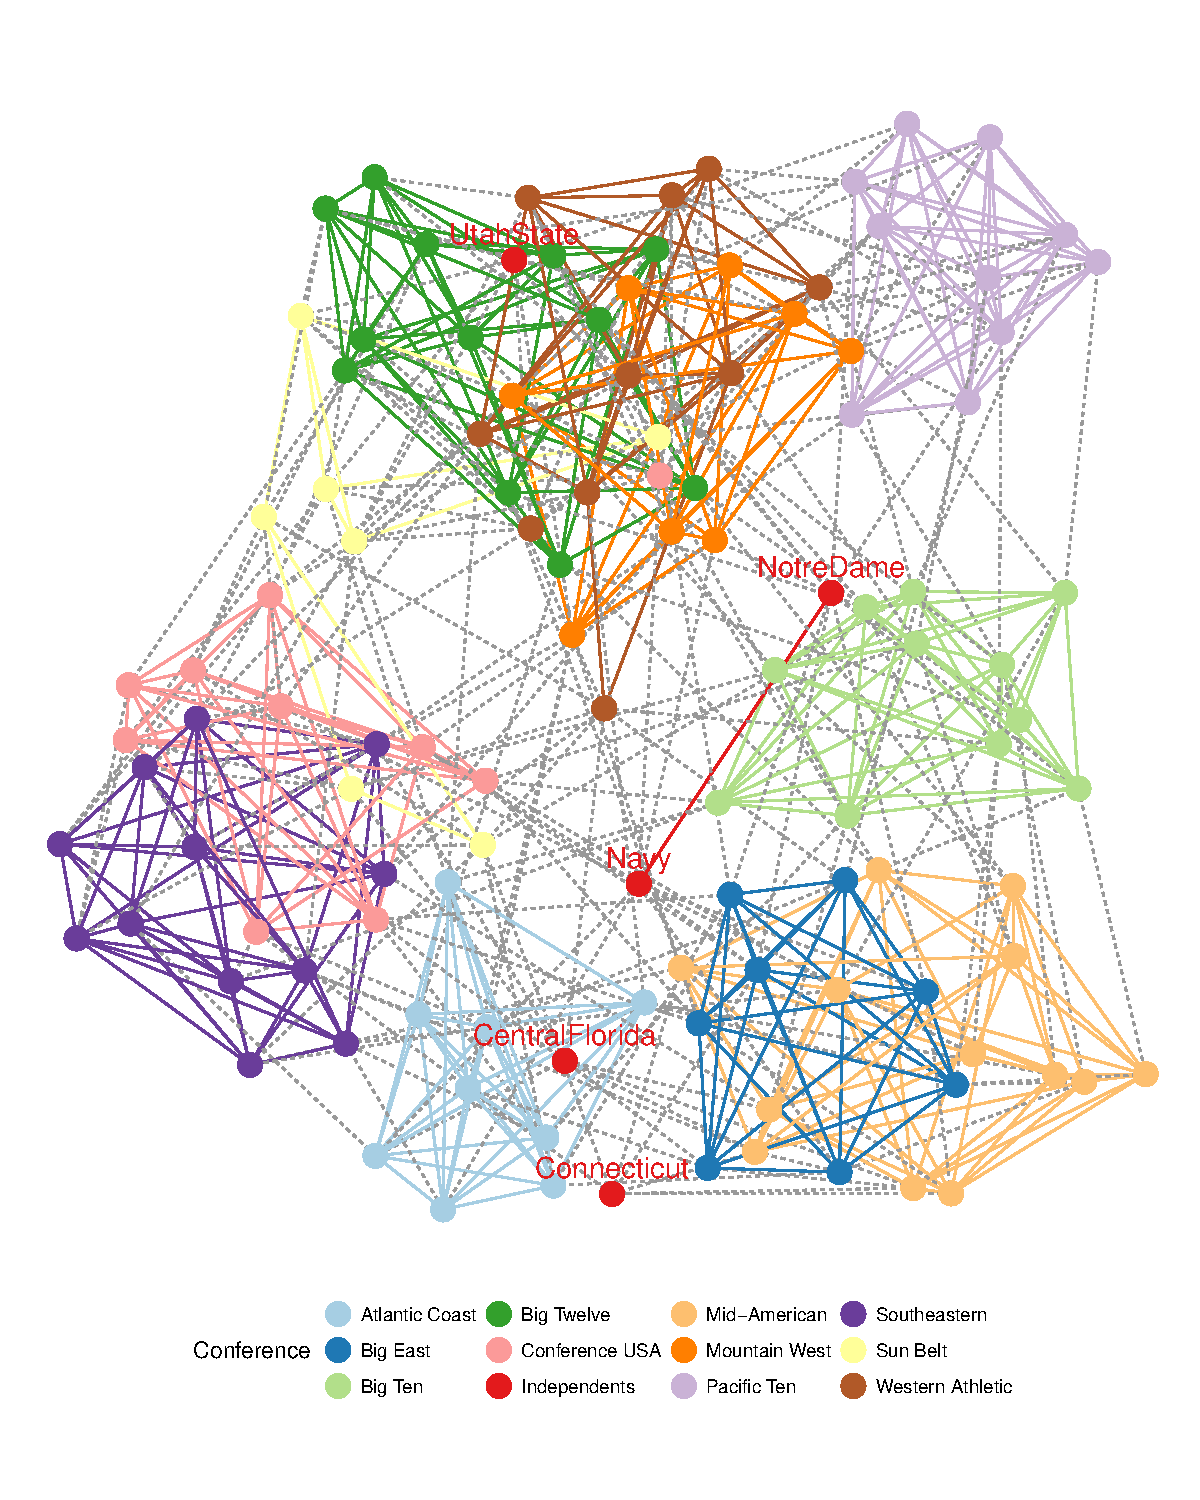
\includegraphics[width=\textwidth]{figure/football_geom_net-1.pdf}

                          \end{minipage}

                          \end{adjustbox}
\end{subfigure}
%
\begin{subfigure}[t]{\textwidth}
\caption{ggnetwork}\vspace{-.5cm}

%%%%%%%%%%%%%
% SCT # out of conf. games connected by dotted lines, not the other way around
\vspace{1em}

             \begin{adjustbox}{valign=t}

             \begin{minipage}{.49\textwidth}
 \begin{knitrout}\footnotesize
\definecolor{shadecolor}{rgb}{1, 1, 1}\color{fgcolor}\begin{kframe}
\begin{verbatim}
ggplot(
  ggnetwork(fb.net, layout = "fruchtermanreingold"),
  aes(x, y, xend = xend, yend = yend)) +
  geom_edges(
    aes(linetype = as.factor(same.conf)),
    color = "grey50") +
  geom_nodes(aes(color = conf), size = 4) +
  scale_color_brewer("Conference",
                     palette = "Paired") +
    scale_linetype_manual(values = c(2,1)) +
  guides(linetype = FALSE) +
  theme_blank()
\end{verbatim}
\end{kframe}
\end{knitrout} \vspace{1em}

                   \end{minipage}

                  \begin{minipage}{.49\textwidth}

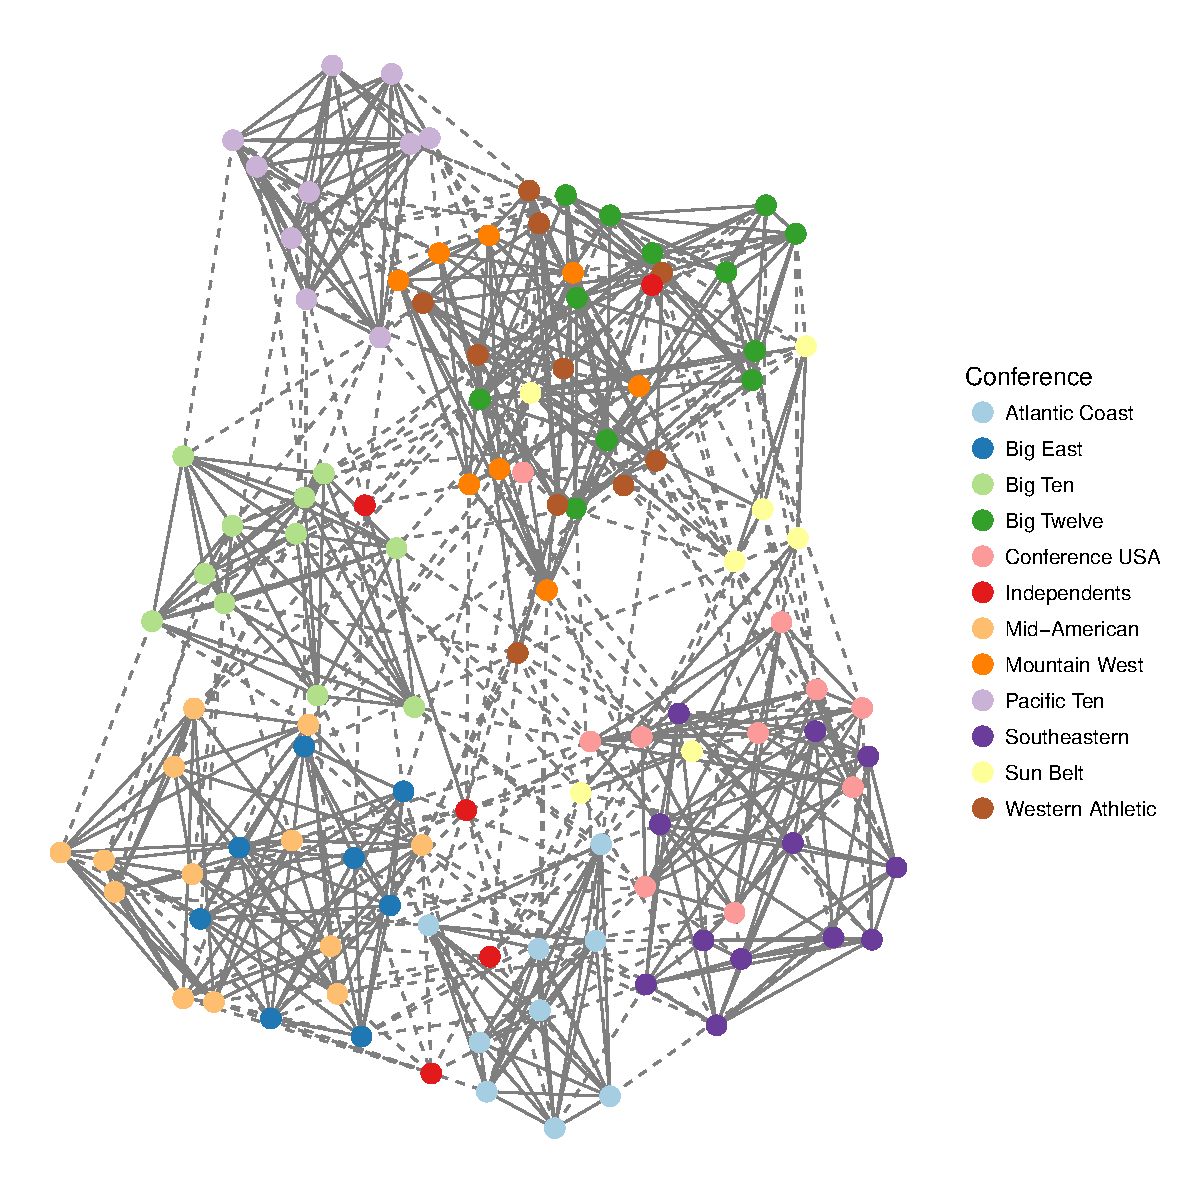
\includegraphics[width=\textwidth]{figure/football_ggnetwork-1.pdf}

                          \end{minipage}

                          \end{adjustbox}
\end{subfigure}
\caption{\label{fig.cap:football} The network of regular season Division I college football games in the season of fall 2000. The vertices and their labels are colored by conference.}
\end{figure}
\afterpage{\clearpage}

%' \subsection{Character co-appearances in \emph{Les Mis\'{e}rables}} % ===========
%' 
%' \fb{XXX Please don't get mad at me: I think we discussed that earlier, but I'm still unable to see what this ex. brings to the paper. What does it show that is not shown in the other examples? XXX}
%' 
%' \sct{XXX Fran\c{c}ois, I can see that. The original intent was to demonstrate the ability of the geom to change edge widths based on some weight variable. But, this is also done now in the bike share example, which also happens to be a much cooler and more unique example. XXX}
%' 
%' %This next network comes from \citet{lesmis}. It is an undirected network of coappearances of characters in Victor Hugo's \emph{Les Mis\'{e}rables}.  There are 77 vertices representing each of the 77 characters in the book, and an edge connects two vertices if those two characters appear in the same chapter of the book.  There are 254 edges in this network. The edges are also weighted by the number of coappearances. The largest weighting is 31, between the characters Jean Valjean and Cosette.
%' %This network is shown in Figures~\ref{fig.cap:lesmis:ggnet2},~\ref{fig.cap:lesmis:ggnet}, and~\ref{fig.cap:lesmis:ggnetwork}; the corresponding code is shown below. This network reveals many important character groups, as well as the main characters in the story.  The main characters are the ones with high degree, like Valjean, Cosette, and Javert.  There is an extremely wide edge connecting Valjean and Cosette, which implies that they are strongly connected; in fact, Cosette is Valjean's adopted daughter.
%' 
%' \hh{not mad :)  what I like about this example is that it is a classic, and it also does not have one single perfect solution. The number of edges and the length of the node labels makes it quite tricky to lay out nicely. I like the fact that we have three different approaches to that. But I'm also not totally opposed to removing the example.}
%' 
%' % This example is a classic published by \citet{lesmis}. It is an undirected network of coappearances of characters in Victor Hugo's \emph{Les Mis\'{e}rables}.  There are 77 vertices representing each of the 77 characters in the book, and an edge connects two vertices if those two characters appear in the same chapter of the book.  There are 254 edges in this network. The edges are also weighted by the number of coappearances. The largest weighting is 31, between the characters Jean Valjean and Cosette.
%' % This network is shown in Figures~\ref{fig.cap:lesmis:ggnet2},~\ref{fig.cap:lesmis:ggnet}, and~\ref{fig.cap:lesmis:ggnetwork}; the corresponding code is shown below. This network reveals many important character groups, as well as the main characters in the story.  The main characters are the ones with high degree, like Valjean, Cosette, and Javert.  There is an extremely wide edge connecting Valjean and Cosette, which implies that they are strongly connected; in fact, Cosette is Valjean's adopted daughter.
%' 
%' 
%' % \begin{figure}[hbtp]
%' % \caption{\label{tab:lesmis}Code for the three approaches of visualizing the relationships between characters in Les Mis\'{e}rables as shown in Figures~\ref{fig.cap:lesmis:ggnet2},~\ref{fig.cap:lesmis:ggnet}, and~\ref{fig.cap:lesmis:ggnetwork}.}
%' <<lesmis_ggnet2, echo=TRUE>>=
%' # Code for the three visualization approaches of co-appearances
%' # plot with ggnet2
%' ggnet2(lesmis$edges[, 1:2 ], mode = "fruchtermanreingold",
%'        color = "white", label = TRUE, label.color = "grey30",
%'        edge.size = lesmis$edges$degree / mean(lesmis$edges$degree),
%'        edge.color = "grey60",
%'        layout.exp = 0.25)
%' @
%' 
%' <<lesmis_geom_net, echo=TRUE, fig.width=9.5>>=
%' # plot with geom_net
%' # data step: merge vertices and edges
%' lesmisnet <- merge(lesmis$edges, lesmis$vertices, by.x = "from",
%'                    by.y = "label", all = TRUE)
%' lesmisnet$degree[ is.na(lesmisnet$degree) ] <- 0
%' 
%' # create plot
%' ggplot(data = lesmisnet, aes(from_id = from, to_id = to,
%'                              linewidth = degree / 5 + 0.1 )) +
%'   geom_net(aes(size = degree, alpha = degree),
%'            colour = "grey30", ecolour = "grey60",
%'            layout = "fruchtermanreingold", label = TRUE, vjust = -0.75) +
%'   scale_alpha(range = c(0.3, 1)) +
%'   theme_net()
%' @
%' 
%' %% not sure I understand the aesth. mapping used above, so not using alpha below
%' <<lesmis_ggnetwork, echo=TRUE, fig.width=9.5>>=
%' # plot with ggnetwork
%' ggplot(data = ggnetwork(lesmis$edges[, 1:2 ], arrow.gap = 0),
%'        aes(x, y, xend = xend, yend = yend)) +
%'   geom_edges(size = lesmis$edges$degree / mean(lesmis$edges$degree),
%'              color = "grey60") +
%'   geom_nodes(color = "white", size = 6) +
%'   geom_nodetext(aes(label = vertex.names), color = "grey30") +
%'   theme_blank()
%' @
%' %\end{figure}
%' %
%' % \begin{figure}[hbtp]
%' % \includegraphics[width=\textwidth]{figure/lesmis_ggnet2-1.pdf}
%' % \caption{\label{fig.cap:lesmis:ggnet2} Co-appearance network of characters in Victor Hugo's \emph{Les Mis\'{e}rables} using ggnet2.}
%' % \end{figure}
%' % %
%' % \begin{figure}[hbtp]
%' % \includegraphics[width=\textwidth]{figure/lesmis_geom_net-1.pdf}
%' % \caption{\label{fig.cap:lesmis:ggnet} Co-appearance network of characters in Victor Hugo's \emph{Les Mis\'{e}rables} using geomnet.}
%' % \end{figure}
%' % %
%' % \begin{figure}[hbtp]
%' % \includegraphics[width=\textwidth]{figure/lesmis_ggnetwork-1.pdf}
%' % \caption{\label{fig.cap:lesmis:ggnetwork} Co-appearance network of characters in Victor Hugo's \emph{Les Mis\'{e}rables} using ggnetwork.}
%' % \end{figure}
%' %
%' %\afterpage{\clearpage}

\subsection{Bikesharing in Washington D.C.} % ==================================

The data shows trips taken with bikes from the bike share company Capital Bikeshare\footnote{\url{https://secure.capitalbikeshare.com/}} during the second quarter of 2015.
While this bikesharing company is located in the heart of Washington D.C.\ the company offers a set of bike stations just outside of Washington in Rockville, MD and north of it. Each station is shown as a vertex, and edges between stations indicate that at least five trips were taken between these two stations; the wider the line, the more trips have been taken between stations. In order to reflect distance between stations, we use as an additional restriction that the fastest trip was at most ten minutes long.
Figure~\ref{fig:bikes} shows four renderings of this data. The first is a geographically true representation of the area overlaid by lines between bike stations, the other three are networks drawn with \pkg{geomnet}, \pkg{ggnet2}, and \pkg{ggnetwork}, respectively.
The code for these renderings is shown below.

\begin{knitrout}
\definecolor{shadecolor}{rgb}{1, 1, 1}\color{fgcolor}\begin{kframe}
\begin{verbatim}
# code for geomnet
# data preparation
tripnet <- merge(bikes$trips, bikes$stations, by.x = "Start.station",
                 by.y = "name", all = TRUE)

tripnet$Metro = FALSE
idx <- grep("Metro", tripnet$Start.station)
tripnet$Metro[idx] <- TRUE

# plot the bike sharing network
ggplot(aes(from_id = Start.station, to_id = End.station), data = tripnet) +
  geom_net(aes(linewidth = n / 15, colour = Metro),
           label = TRUE, vjust = -0.5) +
  theme_net() +
  xlim(c(-0.1, 1.1)) +
  scale_colour_manual("Metro Station", values = c("grey40", "darkorange")) +
  theme(legend.position = "bottom")
\end{verbatim}
\end{kframe}
\end{knitrout}


\begin{knitrout}
\definecolor{shadecolor}{rgb}{1, 1, 1}\color{fgcolor}\begin{kframe}
\begin{verbatim}
# data preparation for ggnet2 and ggnetwork
bikes.net <- network(bikes$trips[, 1:2 ], directed = FALSE)
set.edge.attribute(bikes.net, "n", bikes$trips[, 3 ] / 15)
bikes.net %v% "station" <-
  grepl("Metro", network.vertex.names(bikes.net))
bikes.net %v% "station" <-
  1 + as.integer(bikes.net %v% "station")
rownames(bikes$stations) <- bikes$stations$name
bikes.net %v% "lon" <-
  bikes$stations[ network.vertex.names(bikes.net), "long" ]
bikes.net %v% "lat" <-
  bikes$stations[ network.vertex.names(bikes.net), "lat" ]
bikes.col <- c("grey40", "darkorange")
\end{verbatim}
\end{kframe}
\end{knitrout}

\begin{knitrout}
\definecolor{shadecolor}{rgb}{1, 1, 1}\color{fgcolor}\begin{kframe}
\begin{verbatim}
# Fruchterman-Reingold placement
ggnet2(bikes.net, size = 4, label = TRUE, vjust = -0.5,
       edge.size = "n", color = bikes.col[ bikes.net %v% "station" ],
       label.color = bikes.col[ bikes.net %v% "station" ],
       layout.exp = 1.1)
\end{verbatim}
\end{kframe}
\end{knitrout}

\begin{knitrout}
\definecolor{shadecolor}{rgb}{1, 1, 1}\color{fgcolor}\begin{kframe}
\begin{verbatim}
# Fruchterman-Reingold placement
ggplot(data = ggnetwork(bikes.net),
       aes(x, y, xend = xend, yend = yend)) +
  geom_edges(aes(size = n), color = "grey40") +
  geom_nodes(aes(color = factor(station)), size = 4) +
  geom_nodetext(aes(label = vertex.names, color = factor(station)),
                vjust = -0.5) +
  scale_size_continuous("Trips", breaks = c(2, 4, 6), labels = c(30, 60, 90)) +
  scale_colour_manual("Metro station", labels = c("FALSE", "TRUE"),
                      values = c("grey40", "darkorange")) +
  theme_blank() +
  theme(legend.position = "bottom", legend.box = "horizontal")
\end{verbatim}
\end{kframe}
\end{knitrout}

For the geographic representations we also made use of the three packages. Because all three approaches result in the same picture, we only show one of these in figure~\ref{fig:bikes}a. The code is given here.

%% FB: separated block below into four blocks, as we did for the blood example
\begin{knitrout}
\definecolor{shadecolor}{rgb}{1, 1, 1}\color{fgcolor}\begin{kframe}
\begin{verbatim}
data(metro_map)
\end{verbatim}
\end{kframe}
\end{knitrout}
%
\begin{knitrout}
\definecolor{shadecolor}{rgb}{1, 1, 1}\color{fgcolor}\begin{kframe}
\begin{verbatim}
# geomnet: overlay bike sharing network on geographic map
ggplot(data = metro_map, aes(x = x, y = y)) +
  geom_raster(fill = metro_map$fill, alpha = 0.75) +
  geom_net(data = tripnet, layout = NULL, label = TRUE,
           vjust = -0.5, ealpha = 0.5,
           aes(from_id = Start.station,
               to_id = End.station,
               x = long, y = lat,
               linewidth = n / 15,
               colour = Metro)) +
  scale_colour_manual("Metro Station", values = c("grey40", "darkorange")) +
  theme_net() %+replace% theme(aspect.ratio=NULL) +
  theme(legend.position = "bottom")
\end{verbatim}
\end{kframe}
\end{knitrout}
\begin{knitrout}
\definecolor{shadecolor}{rgb}{1, 1, 1}\color{fgcolor}\begin{kframe}
\begin{verbatim}
# geographic placement using ggnet2
ggnet2(bikes.net, size = 4, label = TRUE, vjust = -0.5,
       mode = c("lon", "lat"),
       edge.size = "n",
       color = bikes.col[ bikes.net %v% "station" ],
       label.color = bikes.col[ bikes.net %v% "station" ],
       layout.exp = 1.1)
\end{verbatim}
\end{kframe}
\end{knitrout}
\begin{knitrout}
\definecolor{shadecolor}{rgb}{1, 1, 1}\color{fgcolor}\begin{kframe}
\begin{verbatim}
# geographic placement using ggnetwork
coords <- c(bikes.net %v% "lon", bikes.net %v% "lat")
map_01 <- metro_map
map_01$x <- scales::rescale(map_01$x)
map_01$y <- scales::rescale(map_01$y)
ggplot(data = ggnetwork(bikes.net, layout = matrix(coords, ncol = 2)),
       aes(x, y, xend = xend, yend = yend)) +
  geom_raster(data = map_01, aes(x = x, y = y, xend = NULL, yend = NULL),
              fill = map_01$fill, alpha = 0.75) +
  geom_edges(aes(size = n), color = "grey40") +
  geom_nodes(aes(color = factor(station)), size = 4) +
  geom_nodetext(aes(label = vertex.names, color = factor(station)),
                vjust = -0.5) +
  scale_size_continuous("Trips", breaks = c(2, 4, 6), labels = c(30, 60, 90)) +
  scale_colour_manual("Metro station", labels = c("FALSE", "TRUE"),
                      values = c("grey40", "darkorange")) +
  scale_x_continuous(limits = c(-0.1, 1.1)) +
  scale_y_continuous(limits = c(-0.1, 1.1)) +
  theme_blank() +
  theme(legend.position = "bottom", legend.box = "horizontal")
\end{verbatim}
\end{kframe}
\end{knitrout}
\begin{figure}[hbtp]
\begin{subfigure}[t]{.49\textwidth}
\caption{geographic map}
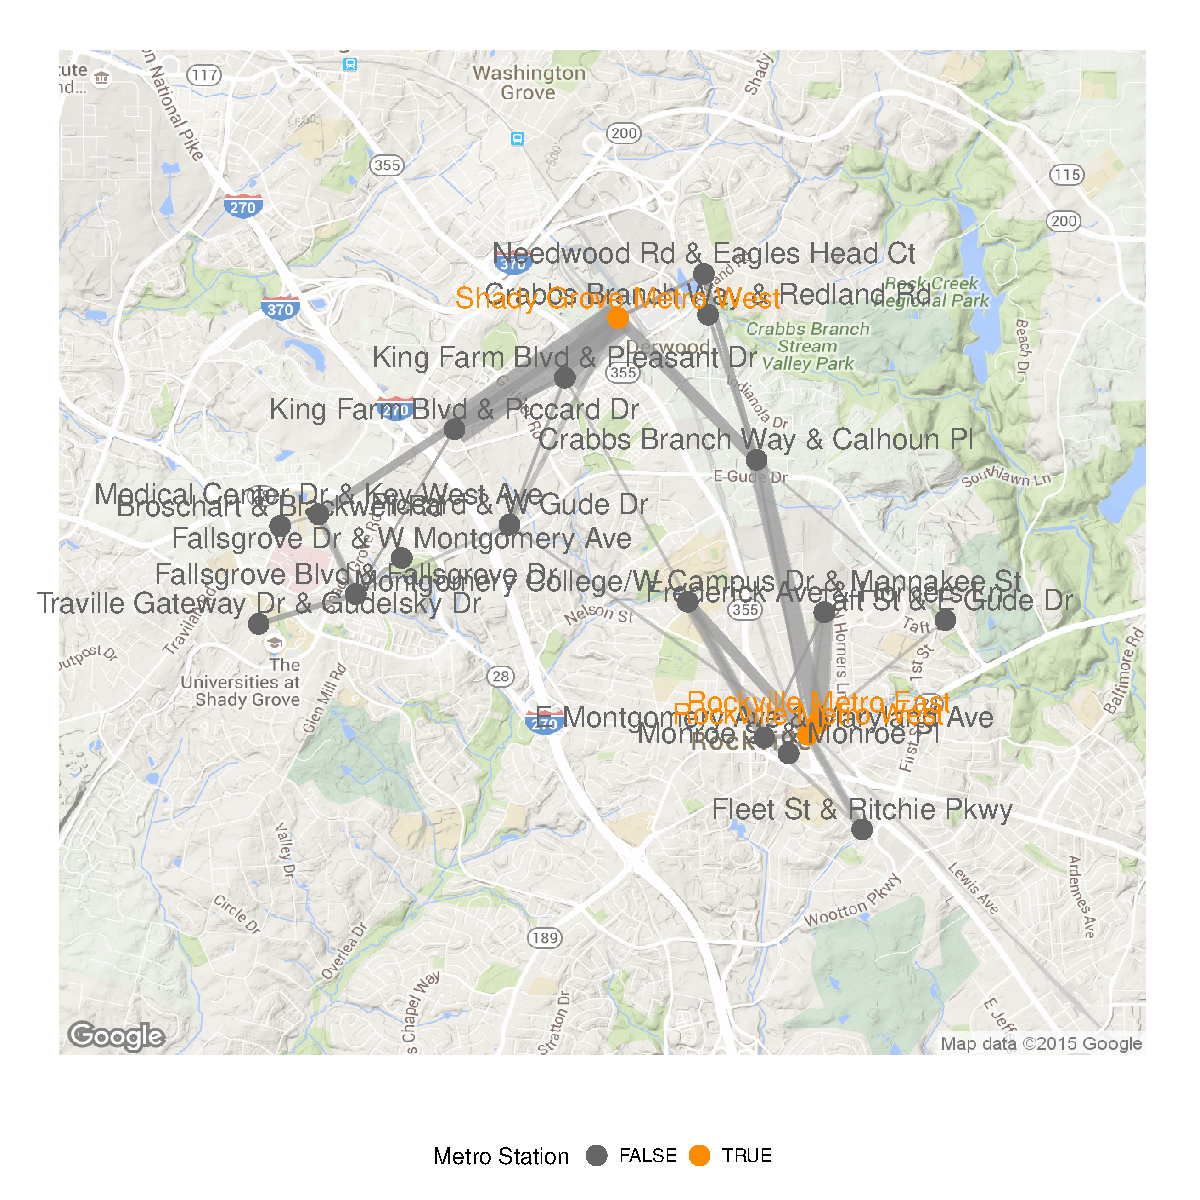
\includegraphics[width=\textwidth]{figure/geographic_geomnet-1.pdf}
\end{subfigure}
\begin{subfigure}[t]{.49\textwidth}
\caption{geomnet}
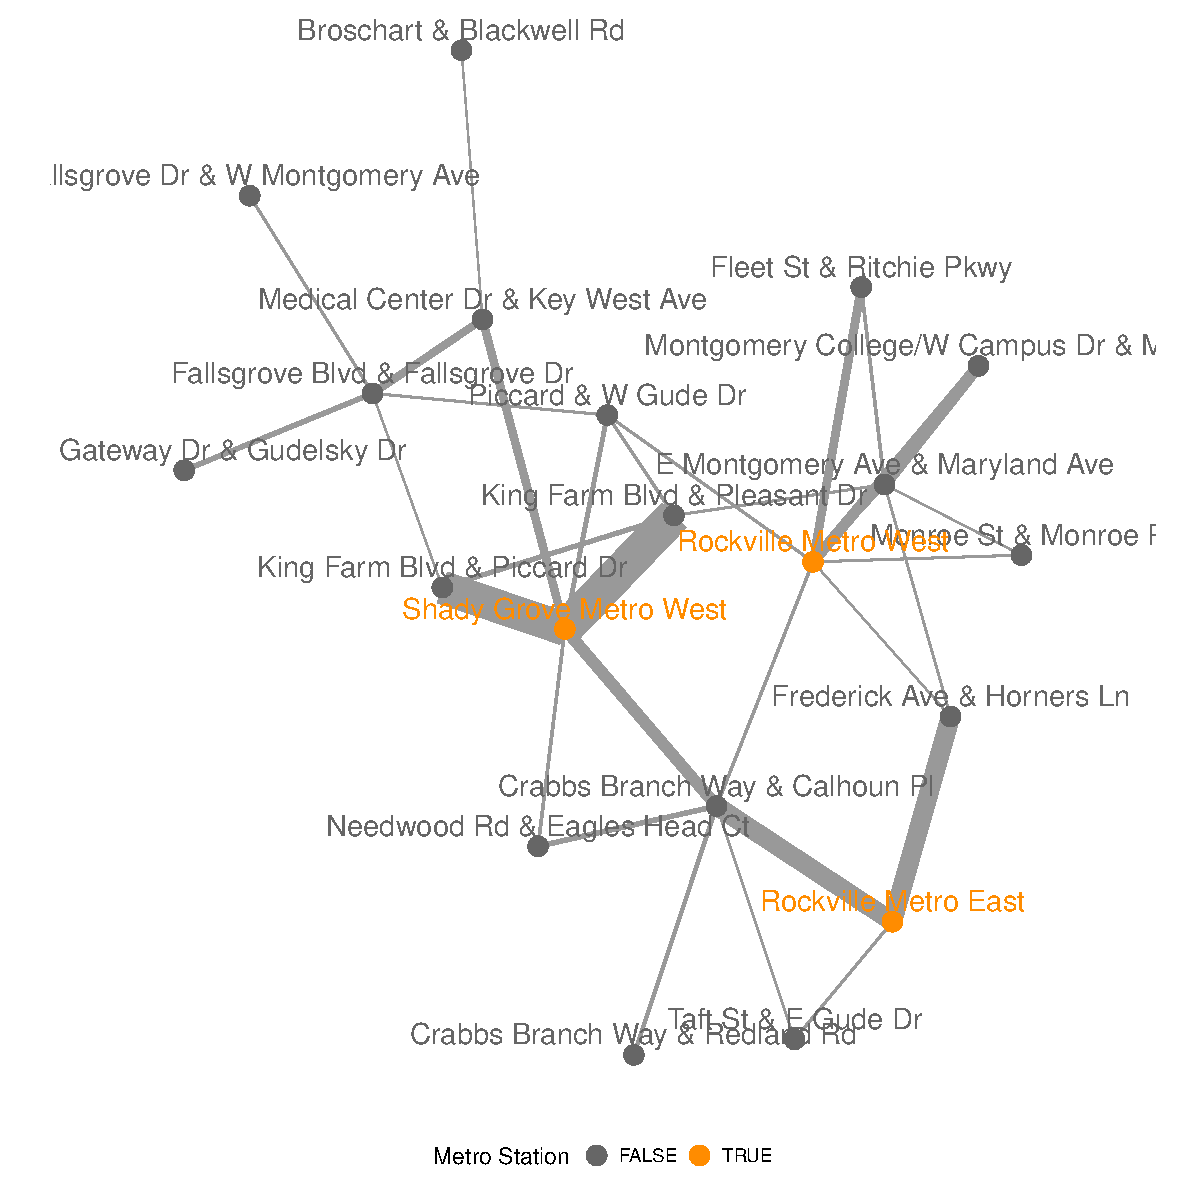
\includegraphics[width=\textwidth]{figure/bikes_geom_net-1.pdf}
\end{subfigure}
\begin{subfigure}[t]{.49\textwidth}
\caption{ggnet2}
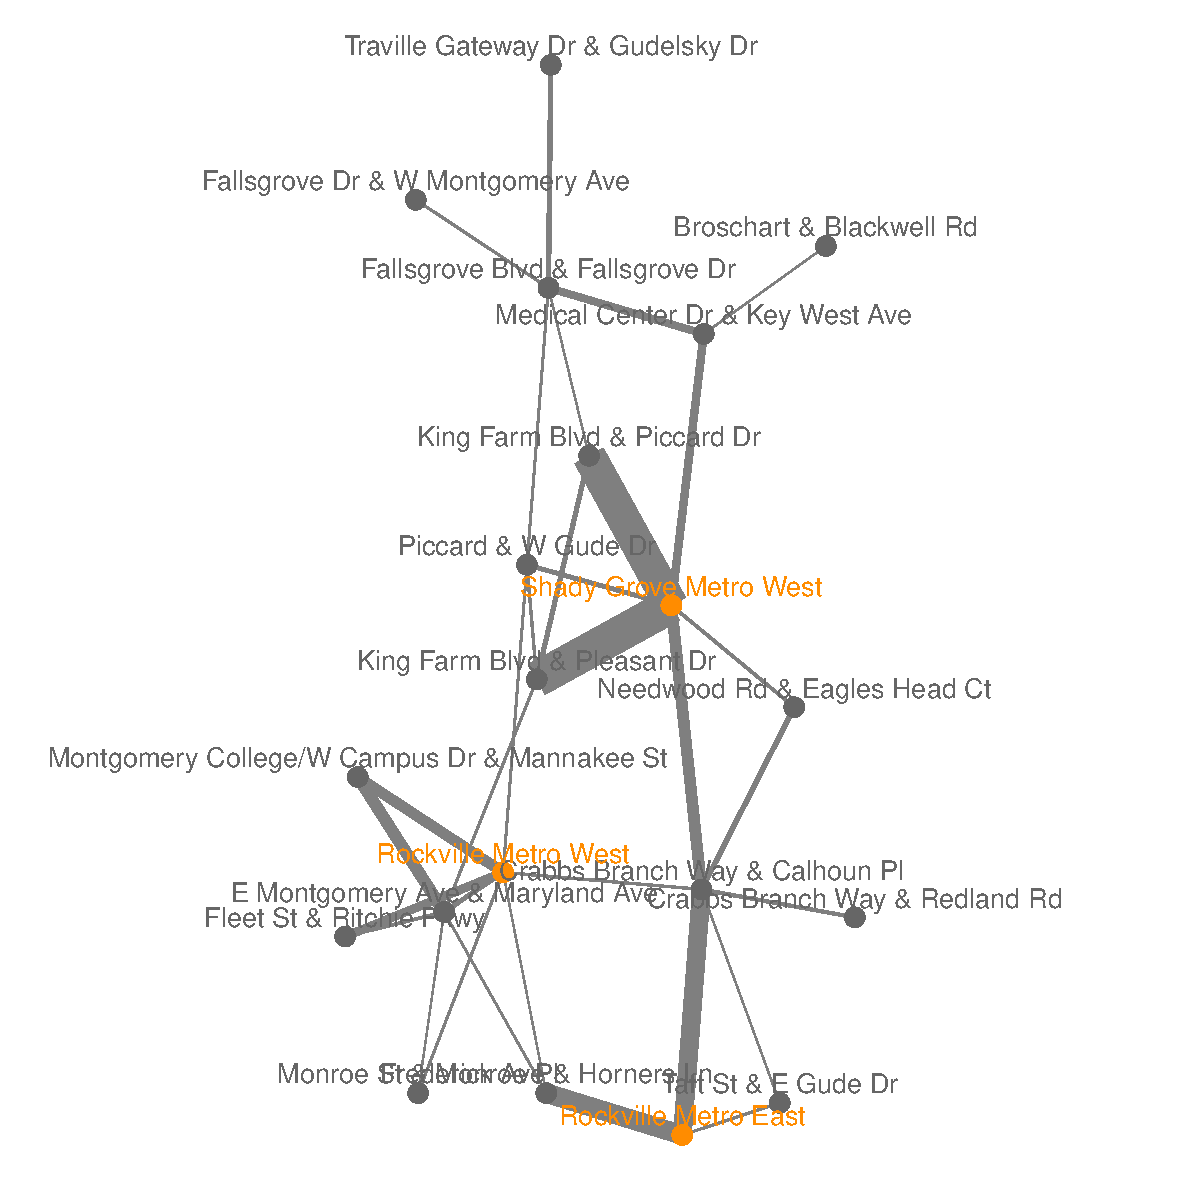
\includegraphics[width=\textwidth]{figure/bikes_ggnet2-1.pdf}
\end{subfigure}
\begin{subfigure}[t]{.49\textwidth}
\caption{ggnetwork}
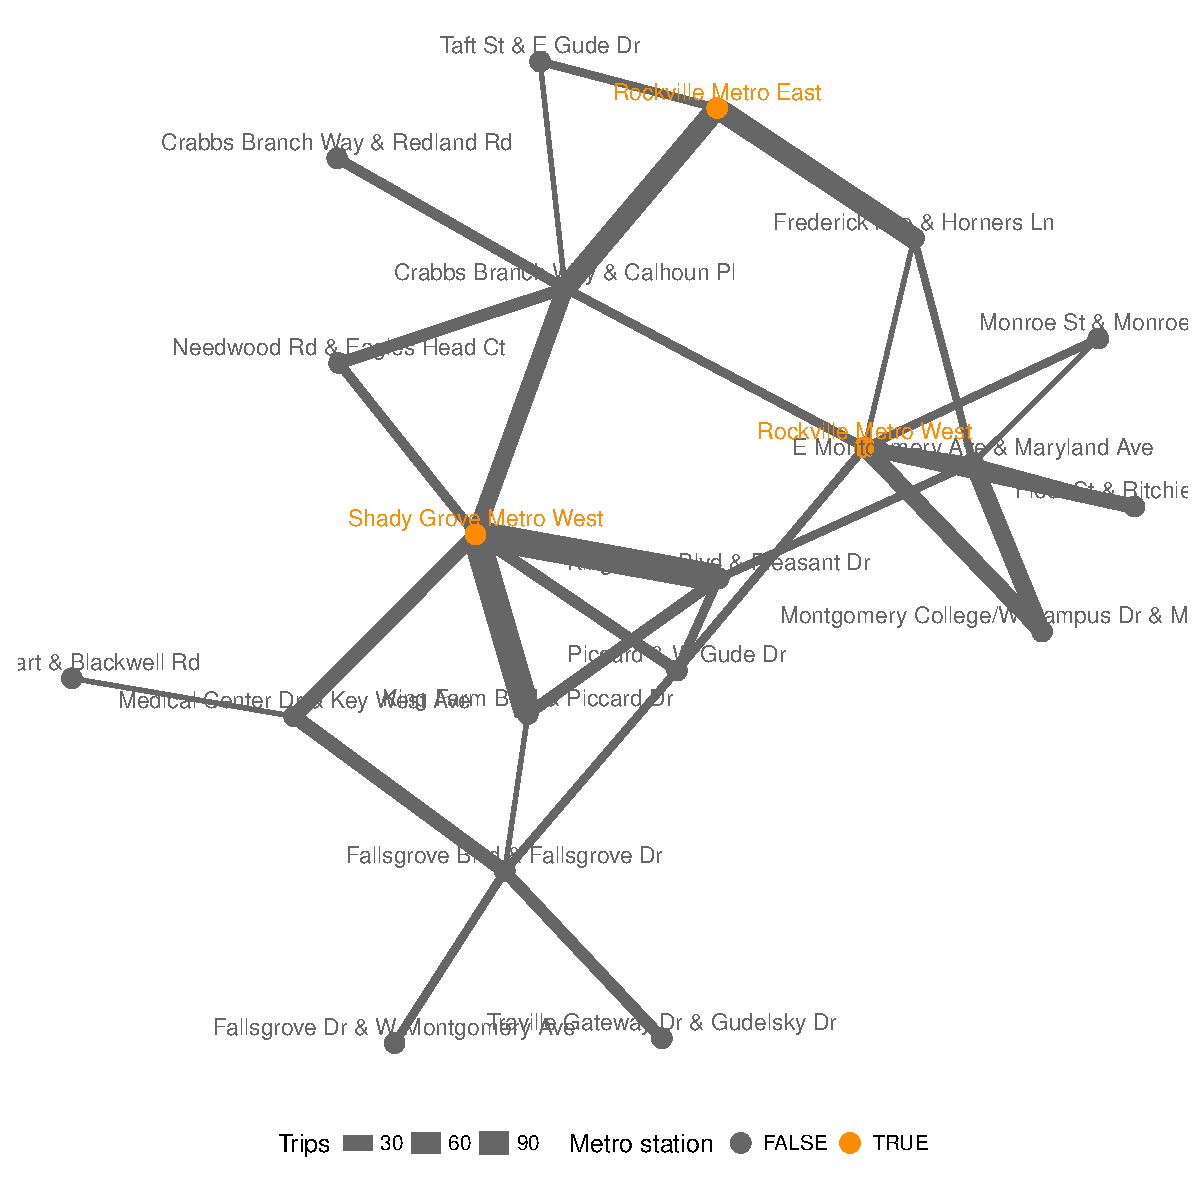
\includegraphics[width=\textwidth]{figure/bikes_ggnetwork-1.pdf}
\end{subfigure}

%\centering
%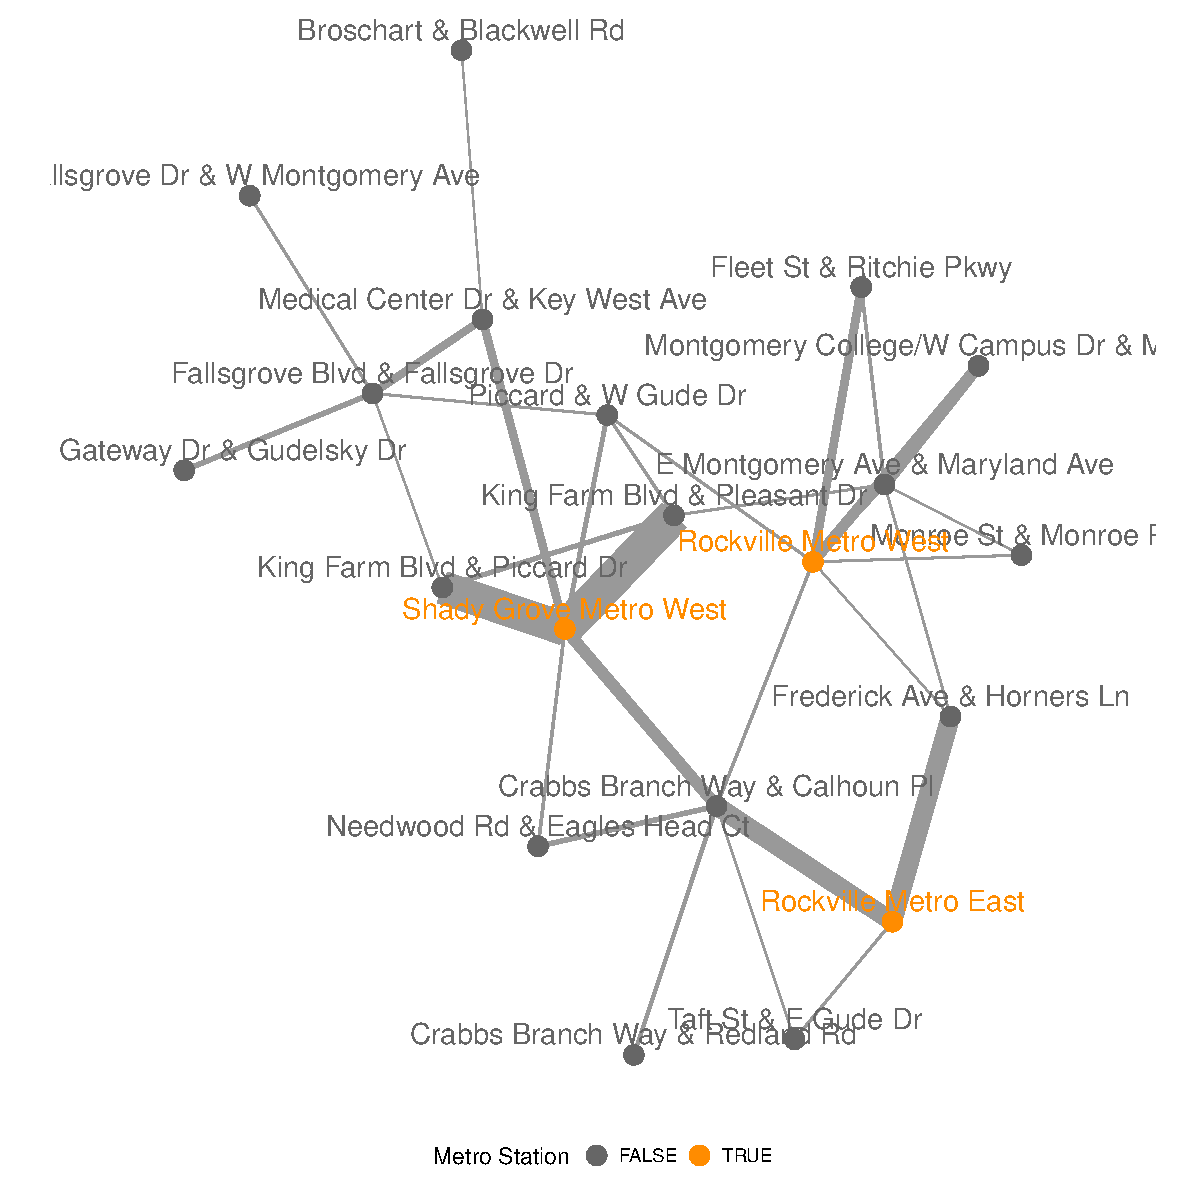
\includegraphics[width=.49\textwidth]{figure/bikes_geom_net-1.pdf}
%\includegraphics[width=.49\textwidth]{figure/bikes_geom_net-2.pdf}
\caption{\label{fig:bikes} Network of bike trips using  a geographically true representation (top left) overlaid on a satellite map, a Kamada-Kawai layout in \pkg{geomnet} (top right), a Fruchterman-Reingold layout in ggnet2 (bottom left) and \pkg{ggnetwork} (bottom right). Metro stations are shown in orange. In both the Kamada-Kawai and the Fruchterman-Reingold layouts, metro stations take a much more central position than in the geographically true representation. }
\end{figure}
%\afterpage{\clearpage}

% \begin{figure}[hbtp]
% \centering
% 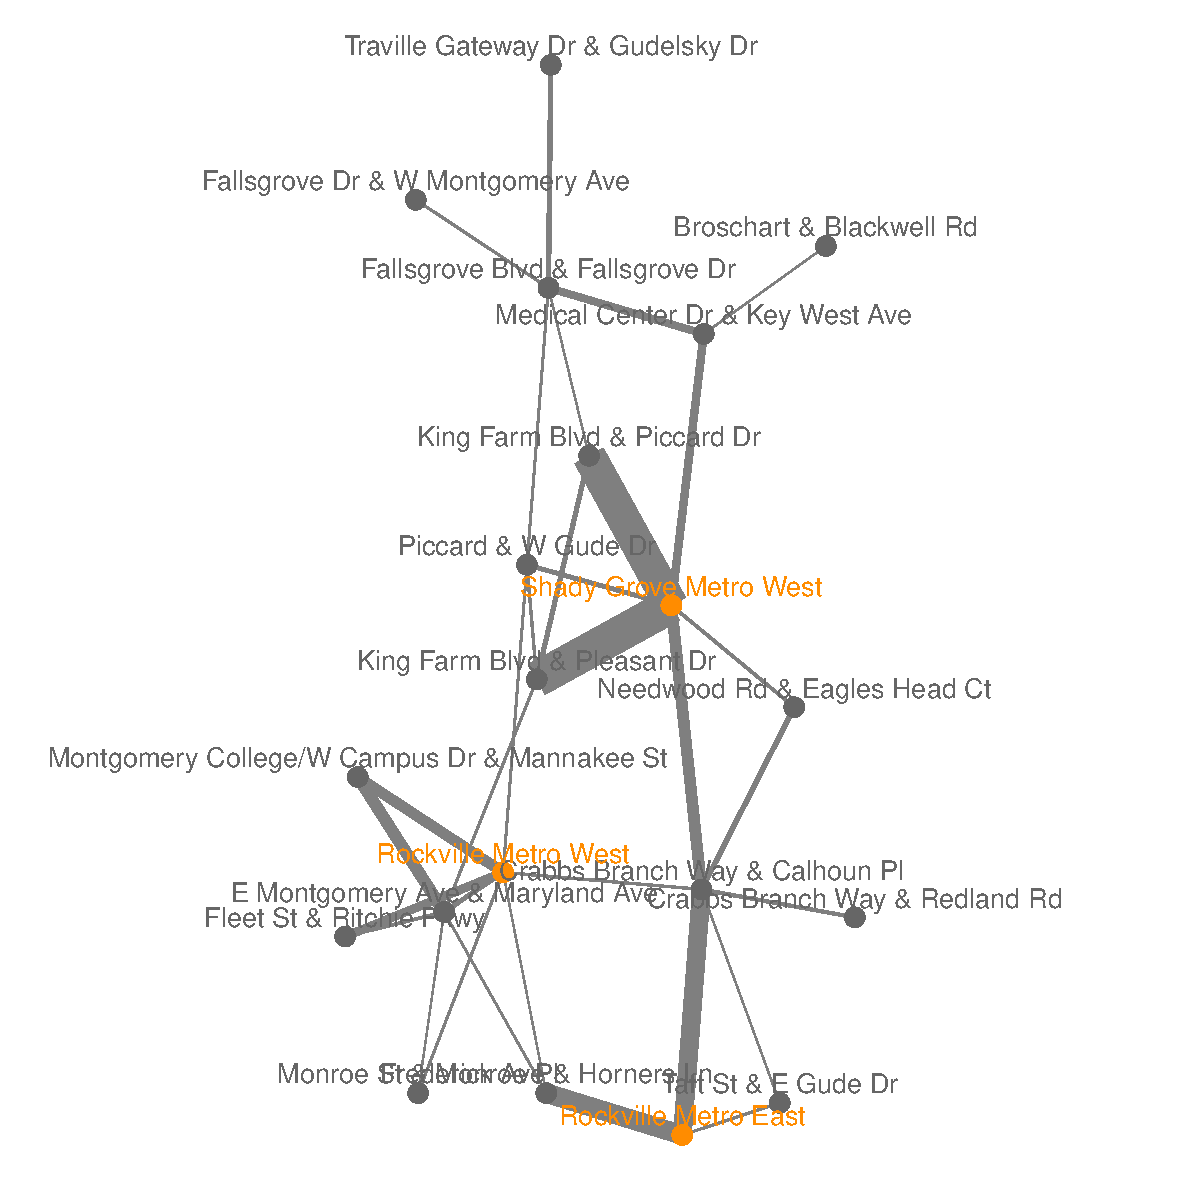
\includegraphics[width=.49\textwidth]{figure/bikes_ggnet2-1.pdf}
% \includegraphics[width=.49\textwidth]{figure/bikes_ggnet2-2.pdf}
% \caption{\label{fig:bikes_ggnet2} ggnet2}
% \end{figure}

% \begin{figure}[hbtp]
% \centering
% 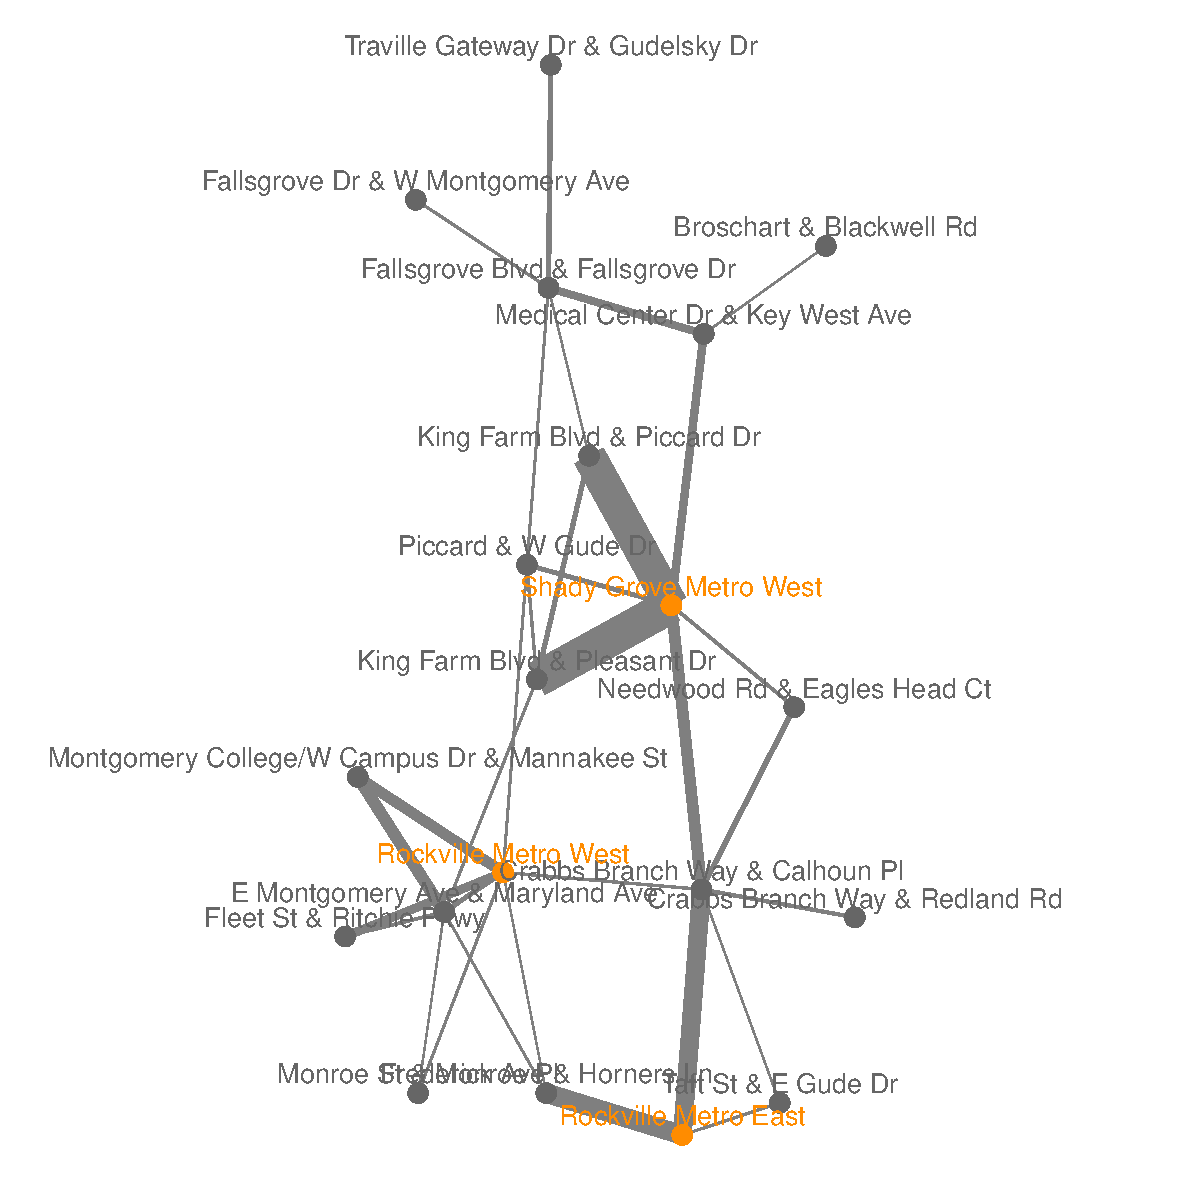
\includegraphics[width=.49\textwidth]{figure/bikes_ggnet2-1.pdf}
% \includegraphics[width=.49\textwidth]{figure/bikes_ggnet2-2.pdf}
% \caption{\label{fig:bikes_ggnetwork} ggnetwork \fb{Problem: standardizing the coordinates to (0,1) distorts the aspect ratio} \hh{have a look at the map - the area covered is actually fairly quadratic. Geographic Lat and Long don't operate on the same scales. } \fb{Still unsure what changes I should bring to make the geographic plot as correct as possible... XYZ} \hh{Shouldn't things on a map have equal distances in x and y? Have a look at the area on the actual map ... it is square - in the image that I'm seeing, the width is about half as wide as it should be.} }
% \end{figure}

\subsection{Protein interactions in yeast} % ===================================

% % \fb{Suggestion: convert this example to a discussion point about speed.}
% % \hh{Talking about speed in the discussion is a good idea, but by the time that we go into the discussion there shouldn't be any more examples. }
% \fb{XXX I understand that the discussion should not introduce additional examples, but I'd still like to move the protein network text to discussion. What I'm suggesting is to lose the protein network as an example of viz-related functionalities (our plots of the network do not introduce any additional functionalities), and just use it as a test support for speed benchmarking at a high network size. See INSERT sentence in discussion for a suggested insert point for the text. XXX}
% \hh{XXX I'd be more in favor of going the opposite way and to drop the discussion of the protein example from the speed considerations. We don't have a handle on the different results, and by them time we do, the protein network is going to be a distraction. I've seen the INSERT point, and I think we could have a sentence there that refers back, if you want, but moving the whole example there is going to make that section even more complicated. XXX}
% \sct{XXX Originally, I added the protein network example for three reasons: first, to demonstrate the layout changes that are possible by passing the layout.par argument to geom\_net; second because it's a pretty well known example of a biological network, which we discuss in the intro; and third, it's a large network, much larger than all of our other ones, and more realistic with respect to what networks many researchers are interested. i.e. more people study networks like this than study networks like the blood, mad men, bikeshare, etc. networks. I think removing it would be detrimental to the paper. I like the idea of keeping it in the examples, adding emphasis to the reasons I put it there in the first place, and referencing it later on. XXX}
% 
In our examples thus far, we have focused on rather small social or relationship networks and one larger communication network. Now we present an example of a biological network, which comes from \citet{protein}. It is the complete protein-protein interaction network in the yeast species \emph{S. cerevisiae}. There are 2,113 proteins that make up the vertices of this network, with a total of 4480 edges between them.  These edges represent ``direct physical interactions" between any two proteins \citep[][p. 42]{protein}, resulting in a relatively large  network. Despite its size, each one of the approaches in the \pkg{ggplot2} framework can be drawn in a few hundred milliseconds. A more in-depth discussion on plotting speed follows in the next section. The proteins and the interactions between them are plotted in the networks shown in Figure~\ref{fig.cap:yeast}. %These interactions and their associated proteins are plotted  in Figure~\ref{fig.cap:yeast}.
In this visualization, we demonstrate the layout capabilities of our functions by changing the layout to \code{random} and setting the distribution to \code{"uniang"}, which is a  ``gaussian donut" layout \citep{sna}.  Indeed, we see a near circular area in the middle of the graph because the layout parameter has forced all of the vertices to the exterior, leaving a ``donut hole" in the middle. Because all of the approaches result in nearly identical figures, only one network is shown. The code for all three approaches is given below:

\begin{knitrout}
\definecolor{shadecolor}{rgb}{1, 1, 1}\color{fgcolor}\begin{kframe}
\begin{verbatim}
# plot with ggnet2
ggnet2(network(protein$edges[,1:2]), size = 2, color = "magenta",
      mode = "random", layout.par = list(dist = "uniang"),
      edge.alpha = 0.05)
\end{verbatim}
\end{kframe}
\end{knitrout}

\begin{knitrout}
\definecolor{shadecolor}{rgb}{1, 1, 1}\color{fgcolor}\begin{kframe}
\begin{verbatim}
# plot with geom_net
ggplot(data = protein$edges, aes(from_id = from, to_id = to)) +
  geom_net(alpha = 0.25, ealpha = 0.05, size = 2, colour = "magenta",
           ecolour = "grey70", linewidth = 0.5,
           layout = "random", layout.par = list(dist = "uniang")) +
  theme_net()
\end{verbatim}
\end{kframe}
\end{knitrout}

\begin{knitrout}
\definecolor{shadecolor}{rgb}{1, 1, 1}\color{fgcolor}\begin{kframe}
\begin{verbatim}
# plot with ggnetwork
ggplot(ggnetwork(protein$edges[, 1:2], layout = "random", dist = "uniang"),
       aes(x, y, xend = xend, yend = yend)) +
  geom_edges(color = "grey70", lwd = 0.5, alpha = 0.05) +
  geom_nodes(alpha = 0.25, color = "magenta", size = 2) +
  theme_blank()
\end{verbatim}
\end{kframe}
\end{knitrout}
\begin{figure}[hbtp]
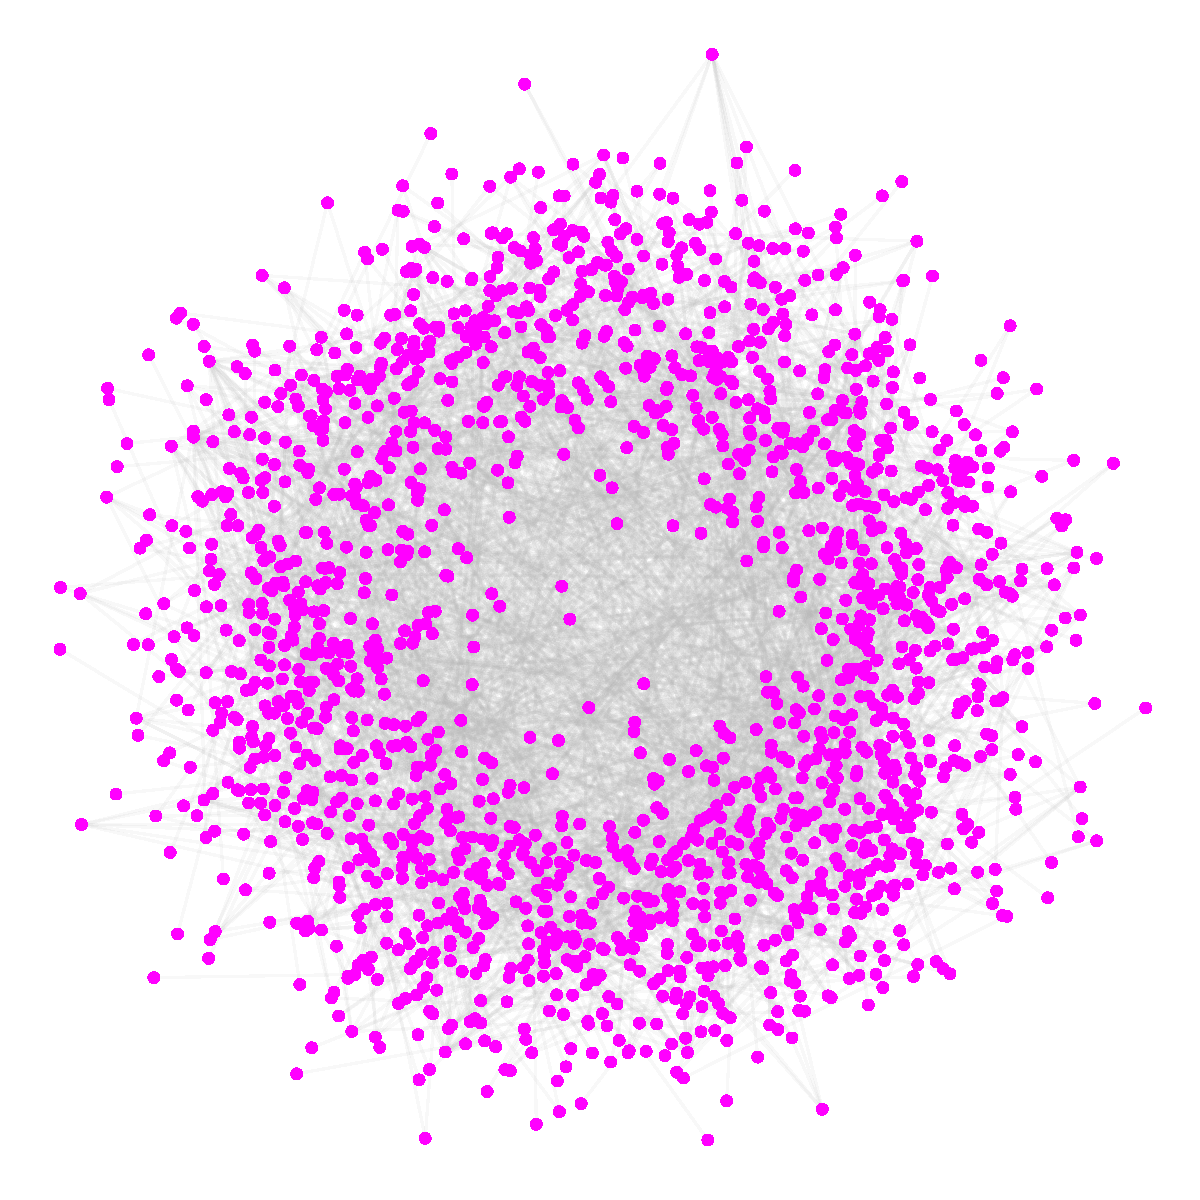
\includegraphics[width=\textwidth]{figure/yeast_geom_net-1.pdf}
%\end{subfigure}
\caption{\label{fig.cap:yeast} Protein-protein interaction network in \emph{S. cerevisiae}. The layout is random and follows a Gaussian donut distributuion.}
\end{figure}
%\afterpage{\clearpage}

%\newpage
\section{Some considerations of speed}\label{sec:speed}
% \hh{XXX So, the testing waters are much more muddy than anticipated. What we can do, though, is to describe the testing scenario(s), and then report our findings with an attempt to summarize. XXX I've added a facetted plot to show the variability in the results that we've seen between the different machines. I made a few changes to the plot, as you can see - using a smooth allows us to see a trend, while the points show variability and give some indication of the distribution (I don't like min and max for that because they are the least robust measures). I also want to see where the actual measurements are taken - that's the reason for showing the points. XXX}

Another benefit that emerges from using \pkg{ggplot2} for network visualization is the speed at which it can plot fairly large networks. In order to assess the speed gain procured by our three approaches, we ran two separate tests, both of which designate \pkg{ggplot2}-based approaches as faster than the plotting functionalities offered in the \pkg{network} package. They also show the \pkg{ggplot2} approaches to be largely on par with the speed provided by the \pkg{igraph} package. We first investigate average plotting time
of the protein network%
\footnote{See \url{https://raw.githubusercontent.com/sctyner/ggnet-paper/master/runtimes-protein/run.r} for the code to recreate results for visualizing the protein interaction network.} 
shown in Figure~\ref{fig.cap:yeast}, and then consider average plotting times of increasingly larger random networks. Note that in all tests, default package settings were used.%
\footnote{See \url{https://raw.githubusercontent.com/sctyner/ggnet-paper/master/runtimes/run.r} for code to recreate benchmark results for visualizing random networks.}
%

%so, what should we do? include one of these? or both? I'd support leaving the benchmark code out of the paper, because it is not directly about network viz with ggplot2. Alternately, include it as an appendix? If left out, the code can be referred to by linking to the repo; that's what I would support most.} % $\hh{XXX link to the benchmark code in the repo seems like the best solution -  we should structure the runtime results somewhat and summarize there as well.} DONE - SCT.

We plotted the protein interaction network of Figure~\ref{fig.cap:yeast} 100 times using the \pkg{network} and \pkg{igraph} packages, and compared their run times to 100 runs each of the three visualization approaches introduced in this paper. The results are shown in Figure~\ref{fig:timings}. We can see that on average, the \pkg{ggplot2} framework provides a two to three-fold increase in speed over the network package, and that \pkg{geomnet} and \pkg{ggnetwork} are faster than package \pkg{igraph}. The three \pkg{ggplot2} approaches also have considerably less variability in time than the \pkg{network} package.
Despite the large number of vertices, the protein interaction network has a relatively small number of edges (4480 out of over 2.2 Million theoretically possible connections resulting in an edge probability of just over 0.0020). Next, we examine networks with a higher edge probability.

\begin{figure}
\centering

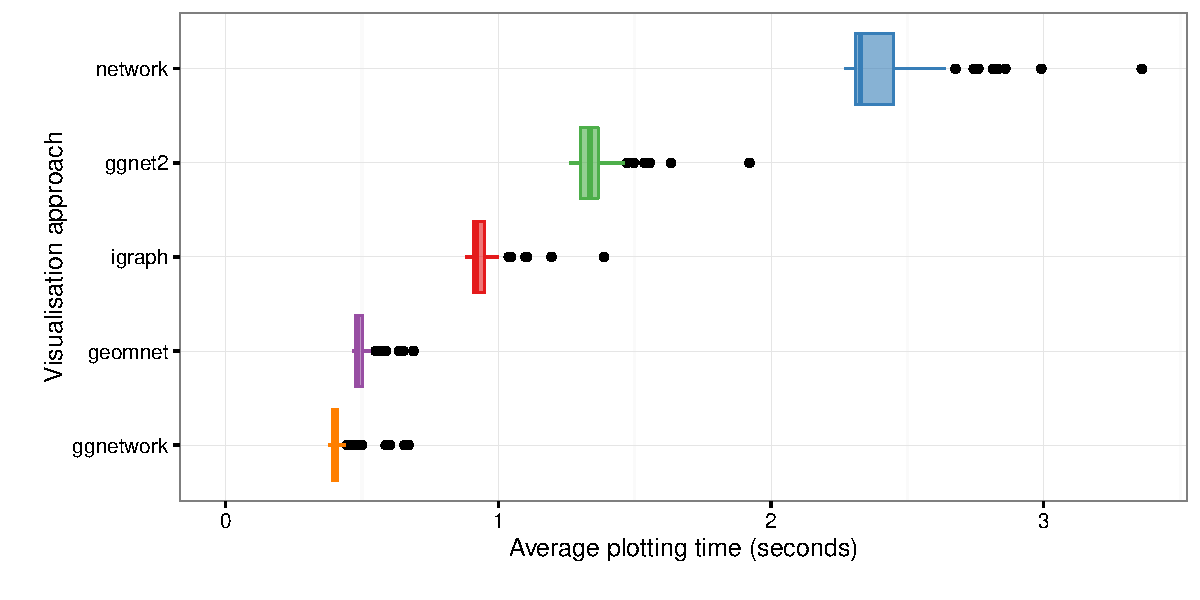
\includegraphics[width=\textwidth]{figure/compare-1.pdf}
\caption{\label{fig:timings} Comparison of the times needed for calculating and rendering the previously discussed protein interaction network in the three \pkg{ggplot2} approaches and the standard plotting routines  of the \pkg{network} and \pkg{igraph} packages based on 100 evaluations each.  }
\end{figure}



%\fb{
%The second test relies on the protein interaction network featured in \citet{protein}, which is the complete protein-protein interaction network in the yeast species \emph{S. cerevisiae}. The network has 1,870 proteins that make up the vertices of the network, with a total of 2,240 edges between them, which represent ``direct physical interactions'' between any two proteins \citep[p. 42]{protein}. These interactions and their associated proteins are plotted in Figure~\ref{fig.cap:yeast} using a random distribution algorithm that produces a ``Gaussian donut'' layout. \fb{The network is shown alongside the execution time of 100 similar plots for each plotting approach.}.
%}

%\fb{-- Include protein figure here, side-to-side with the execution times. Include \pkg{igraph} in the execution times. --}

%\hh{XXX what about the code necessary to produce each one of these networks? I like the fact that this example is extremely concise and would allow us to include the code rather than referring to an external link. My alternative would be: XXX}


%\hh{Additionally, the \pkg{ggplot2} framework provides us with a considerable speed-up compared to the standard plotting routines that come with the \pkg{network} package. We executed the following code 100 times and compared its run time to 100 runs each of the three visualisation approaches introduced in this paper:}
%'
%' <<network-plot, echo = TRUE, eval = FALSE>>=
%' # network package
%' xy = gplot.layout.random(network(protein$edges[, 1:2]),
%'                          layout.par = list(dist = "uniang"))
%' system.time(plot(network(protein$edges[, 1:2]), coord = xy))
%' @
%'
%' <<igraph-plot, echo = TRUE, eval = FALSE>>=
%' # igraph package
%' n = as.matrix(protein$edges[, 1:2])
%' n = igraph::graph_from_edgelist(n, directed = FALSE)
%'
%' system.time(plot(n, vertex.label = NA, layout = layout_randomly))
%' @
%'


The second test relies on random undirected networks in which the probability of an edge %to exist
between two nodes was set to $p = 0.2$.
We generated 100 of these networks at network sizes from 25 to 250 nodes, using increments of 25. %We then computed the average plotting time at each network size.

 %We then computed the average plotting time at each network size, as shown in Figure~\ref{fig.cap:runtimes-random}.

%Although speed was not the main rationale for our inquiry into \pkg{ggplot2}-based approaches to network visualization, a speed-based comparison shows a clear advantage of these approaches over the plotting function included in the \pkg{network} package, which very quickly becomes much slower than when network size increases.

%Further testing on a network of [EDGES] interactions between [NODES] proteins yielded the same conclusion. [INSERT protein-based test here.]



\begin{figure}[hbtp]
\centering

%\includegraphics[width=.5\textwidth]{figure/runtimes-1.pdf}

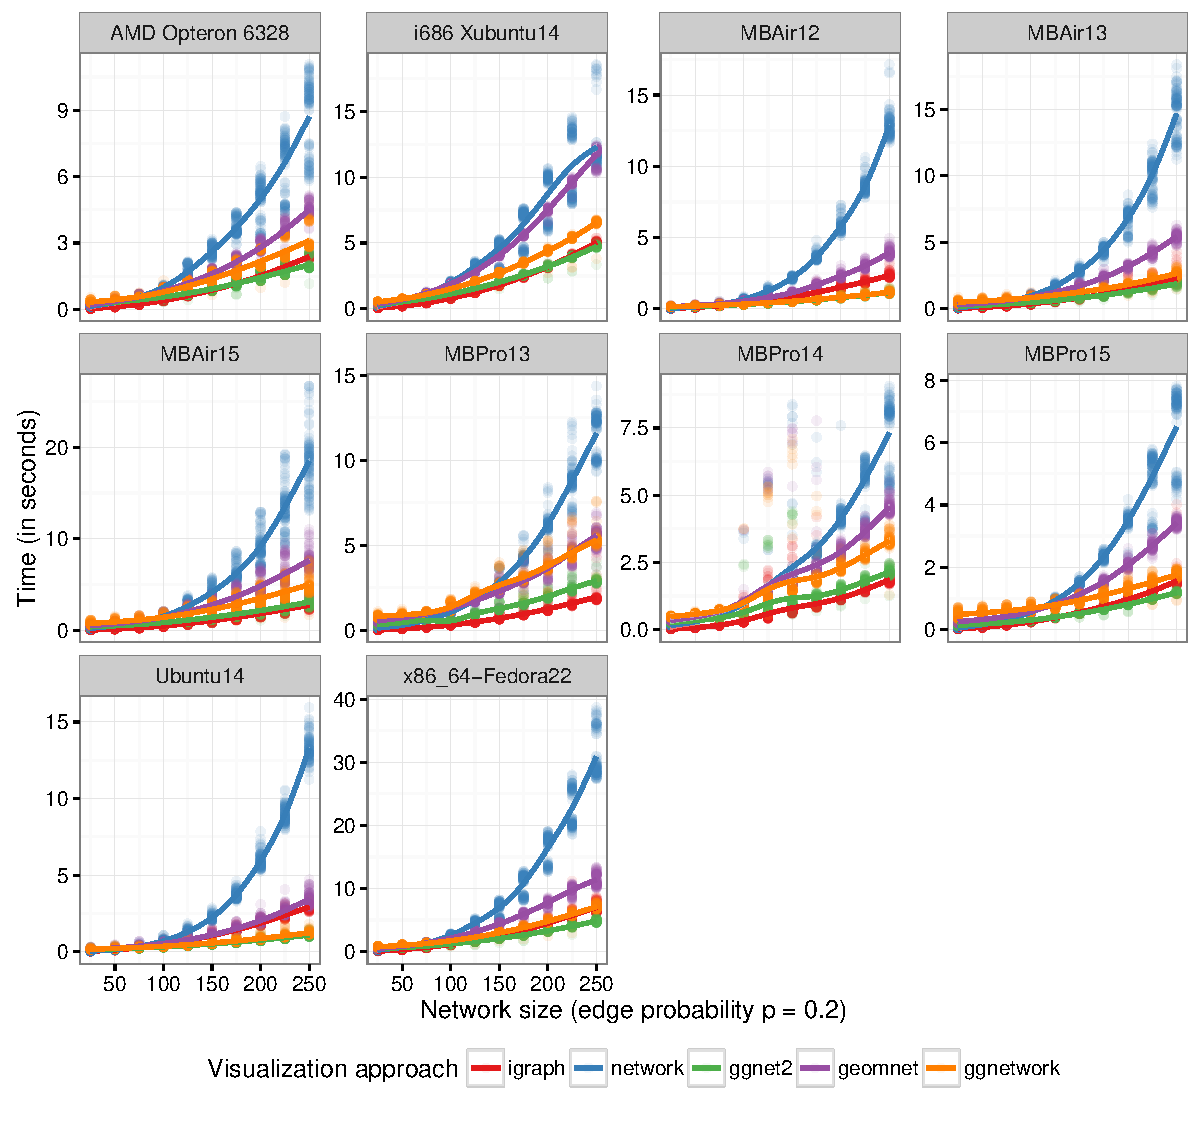
\includegraphics[width=\textwidth]{figure/runtimes-all-1.pdf}
\caption{\label{fig.cap:runtimes-random}%
%  Average plotting time of random undirected networks, in seconds: ribbon at minimum and maximum recorded times, solid line at average. The time ranges of the \code{ggnet2} and \code{ggnetwork} approaches are quasi-identical and form the single purple line at the bottom of the plot.
Plotting times of random undirected networks of different sizes under each of the available visualization approaches using their default settings. Note that each panel is scaled independently to highlight relative differences in the visualization approaches rather than speed of different hardware.
%\fb{Can't remember how I styled the figure in the beginning, but I remember trying to match the previous one by using theme\_classic. We need to harmonize them.} \hh{XXX I'm all for consistency of the figures, but let's please use a theme that has grid lines. They are important for accurate readings. }%
}
\end{figure}

Figure~\ref{fig.cap:runtimes-random} summarizes the results of these benchmarks using a convenience sample of machines accessible to the authors, including authors' hardware and additional results from friends' and colleagues' machines.
Network sizes are plotted horizontally, execution times of 100 runs under each visualization approach are plotted on the $y$-axis. Each panel shows a different machine as indicated by the facet label. Note that each panel is scaled separately to account for differences in the overall speed of these machines.
What these plots indicate is that we have surprisingly large variability in relative run times across different machines.
However, the results support some  general findings.
The \pkg{network} plotting routine is by far the slowest across all machines, while the \pkg{igraph} plotting is generally among the fastest. Our three approaches generally feature in between \pkg{igraph} and \pkg{network} with \pkg{ggnet2} being as fast or faster than \pkg{igraph} plotting, followed by \pkg{ggnetwork} and \pkg{geomnet}, which is generally the slowest among the three. These differences become more pronounced as the size of the network increases.


Although speed was not the main rationale for our inquiry into \pkg{ggplot2}-based approaches to network visualization, a speed-based comparison shows a clear advantage of these approaches over the plotting function included in the \pkg{network} package, which very quickly becomes much slower as network size increases.

% \hh{
% XXX how does edge probability affect these results?
% XXX how do the different layouts affect the results? }


\section{Summary and Discussion}
%\sct{XXX I am going to attempt to pull all of this together into a complete, coherent discussion section.  I removed all of your colors and just kept mine in most places. XXX}



At first  glance, the three visualization approaches may seem nearly identical.
However, %we have seen through our collaboration that HH: should be clear from the paper, too
each one brings unique strengths to the visualization of networks.   Out of our three approaches, \pkg{ggnetwork} is most flexible and allows for a re-ordering of layers to emphasize one over the other. The flexibility is useful but does require the user to specify every single part of the network visualization. The \pkg{geomnet} implementation most closely aligns with the existing \pkg{ggplot2} paradigm because it provides a single layer that can be added to other \code{ggplot2} layers. \pkg{ggnet2} requires the user to know the least about the \pkg{ggplot2} framework, while resulting in a valid and extensible \pkg{ggplot2} object. %\sct{XXX Need more discussion of differing strengths XXX}

%Additionally, 
Many features of the packages would not have been possible, or would have at least been difficult to implement, in  prior versions of \pkg{ggplot2}.  The increased flexibility of the current development version as well as the added \code{geom}s \code{geom\_curve} and \code{geom\_label} provided us with a strong, yet flexible, foundation for network visualization.

These approaches also benefit from the speed of \pkg{ggplot2},  making network visualization more efficient than the existing framework of \pkg{network} for a lot of the benchmark examples. %The \pkg{geomnet} approach is the slower of the three because each call to \code{geom\_net} results in a re-calculation of the network and, unless a seed is set, in a new layout. Once a network layout is calculated in \code{ggnet2} or \code{ggnetwork}, however, subsequent calls to these functions are computationally more efficient because the layout has already been computed.  XXX need a little more XXX

%XXX Add discussion about sna, edgeweights, other plotting functionalities XXX
All three approaches rely on the package \pkg{sna} for layouts. \pkg{sna} unlike the \pkg{network} package supports the use of weights in its edge list.  A larger range of layouts is available through \pkg{igraph}. There are some notable differences between the packages, such as in the parameters used for specific layout algorithms, e.g.\ \pkg{igraph} allows the use of weights for Fruchterman-Reingold placement, even though it is unclear from the original article how these are supposed to affect the layout. In all  three approaches, it is  feasible to tap into \pkg{igraph}'s functionality in a future version.

%\hh{XXX add some discussion on igraph: it is definitely feasible to tap into the functionality of igraph in a future version of geomnet. igraph has, as of June 2015, gone through a major change of its interface, renaming layout functions and the way parameters are handled. }

%\hh{XXX We definitely need to discuss edge weights in the discussion. I am not sure that I have the same take on packages - I would not assume that not being under active development is equivalent to `dormant'.  }

We have found that none of our approaches is unequivocally the best. We can, however, provide some guidance as to which approach is best for which type of user. 
The main differences between the three packages are in the way that network information is passed into the functions. For packages \pkg{ggnet2} and \pkg{ggnetwork} data management and attribute handling is done through network operators on nodes and edges, while the \pkg{geomnet} approach does not require any knowledge of networks or existing network analysis packages from the user. 
This likely affects the user base of each package. 
We think that users who are well-versed with networks will find \pkg{ggnet2} and \pkg{ggnetwork} more intuitive to use. These users might actually be looking to \pkg{ggplot2} to create high-quality visualizations that also have many additional visualization features open to them.


%Since the authors come from two different fields, we have seen how each package fulfills the needs of different user bases. We think that users who are well-versed with networks will find \pkg{ggnet2} and \pkg{ggnetwork} more intuitive to use because data management and attribute handling is done through network operators on nodes and edges. These users might actually be looking to \pkg{ggplot2} to create high-quality visualizations that also have many additional visualization features open to them.  The \pkg{geomnet} approach, on the other hand, does not require any knowledge of networks or existing network analysis packages from the user.   
Users who are already familiar with \pkg{ggplot2} and some of the other `Hadley'-verse package, and who find themselves dealing with data with a network structure will likely be more attracted to the \pkg{geomnet} implementation of network plotting. The data management skills needed for using \pkg{geomnet}are basic: some familiarity with the split-apply-combine paradigm, in the form of familiarity with \pkg{plyr} or \pkg{dplyr}, would be sufficient in order to make full use of the features of \code{geom\_net}. All in all, the three functionalities we have presented here provide a wealth of resources to users of all skill sets who are looking to create beautiful network visualizations.

%  If you are experienced with network analysis in existing R packages and don’t have much experience with \pkg{ggplot2}, then look toward \pkg{ggnet}. If you are not as familiar with network analysis packages but are familiar with visualization in \pkg{ggplot2}, then \pkg{ggnetwork} is for you. And if you don’t know much about network analysis but you do know \pkg{ggplot2}, then your best approach will be \pkg{geomnet}.

On a personal level we discovered that the collaboration on this paper has helped us to improve upon our initial versions of each of these packages. For instance, the edge coloring in the \code{ggnet2} function was designed so that edges between two vertices in the same group were colored with that group's vertex color. This  inspired an implementation of it in \code{geomnet} through the traditional \code{ggplot2} group operator. During the process of writing the paper the authors collaborated on a solution for the problem of nodes being plotted on top of arrow tips. This solution now presents itself in form of the \code{arrow.gap} parameter, which allows to re-track the tip of an arrow on a directed edge.
The implementation of a \pkg{ggplot2} \code{geom} for networks within \pkg{geomnet} inspired the creation of the aliased \code{geom}s of the \pkg{ggnetwork} package. 




\bibliography{tyner-briatte-hofmann}

\address{Samantha Tyner\\
  Department of Statistics and Statistical Laboratory\\
  Iowa State University\\
  United States\\}
\email{sctyner@mail.iastate.edu}

\address{Fran\c{c}ois Briatte\\
  European School of Political Sciences\\
  Catholic University of Lille\\
  France\\}
\email{francois.briatte@univ-catholille.fr}

\address{Heike Hofmann\\
  Department of Statistics and Statistical Laboratory\\
  Iowa State University\\
  United States\\}
\email{hofmann@mail.iastate.edu}
